% ==============================================================================
% Modelo para Tese de Doutorado (em Português)
% Prof. Vítor E. Silva Souza - Nemo / DI / UFES
%
% Baseado em abtex2-modelo-trabalho-academico.tex, v-1.9.2 laurocesar
% Copyright 2012-2014 by abnTeX2 group at http://abntex2.googlecode.com/ 
%
% This work may be distributed and/or modified under the conditions of the LaTeX 
% Project Public License, either version 1.3 of this license or (at your option) 
% any later version. The latest version of this license is in
% http://www.latex-project.org/lppl.txt.
%
% IMPORTANTE:
% Instruções encontram-se espalhadas pelo documento. Para facilitar sua leitura,
% tais instruções são precedidas por (*) -- utilize a função localizar do seu
% editor para passar por todas elas.
% ==============================================================================

% Usa o estilo abntex2, configurando detalhes de formatação e hifenização.
\documentclass[
	12pt,				% Tamanho da fonte.
	openright,			% Capítulos começam em página ímpar (insere página vazia caso preciso).
	twoside,			% Para impressão em verso e anverso. Oposto a oneside.
	a4paper,			% Tamanho do papel.
	english,			% Idioma adicional para hifenização.
	french,				% Idioma adicional para hifenização.
	spanish,			% Idioma adicional para hifenização.
	brazil				% O último idioma é o principal do documento.
	]{abntex2}



%%% Importação de pacotes. %%%
% ---- Inicio import do autor ----
\usepackage{pdflscape}
\usepackage{verbatim}
\usepackage{float}
\usepackage{longtable}
\usepackage{multirow}
\usepackage{multicol}
\usepackage{csquotes}
\usepackage{subcaption}

% ---- Fim import do autor    ----

% Conserta o erro "No room for a new \count"
\usepackage{etex}
% \reserveinserts{28}

% Usa a fonte Latin Modern.
\usepackage{lmodern}

% Seleção de códigos de fonte.
\usepackage[T1]{fontenc}

% Codificação do documento em Unicode.
\usepackage[utf8]{inputenc}

% Usado pela ficha catalográfica.
\usepackage{lastpage}

% Indenta o primeiro parágrafo de cada seção.
\usepackage{indentfirst}

% Controle das cores.
\usepackage[usenames,dvipsnames]{xcolor}

% Inclusão de gráficos.
\usepackage{graphicx}

% Tabularx package: for better control of table layout.
\usepackage{tabularx}

% Inclusão de páginas em PDF diretamente no documento (para uso nos apêndices).
\usepackage{pdfpages}

% Para melhorias de justificação.
\usepackage{microtype}


% Citações padrão ABNT.
\usepackage[brazilian,hyperpageref]{backref}
\usepackage[alf]{abntex2cite}	
\renewcommand{\backrefpagesname}{Citado na(s) página(s):~}		% Usado sem a opção hyperpageref de backref.
\renewcommand{\backref}{}										% Texto padrão antes do número das páginas.
\renewcommand*{\backrefalt}[4]{									% Define os textos da citação.
	\ifcase #1
		Nenhuma citação no texto.
	\or
		Citado na página #2.
	\else
		Citado #1 vezes nas páginas #2.
	\fi}

% \rm is deprecated and should not be used in a LaTeX2e document
% http://tex.stackexchange.com/questions/151897/always-textrm-never-rm-a-counterexample
\renewcommand{\rm}{\textrm}

% Pacotes não incluídos no template abntex2. 
% Podem ser comentados caso não queira utilizá-los.

% Inclusão de símbolos não padrão.
\usepackage{amssymb}
\usepackage{eurosym}

% Para utilizar \eqref para referenciar equações.
\usepackage{amsmath}

% Permite mostrar figuras muito largas em modo paisagem com \begin{sidewaysfigure} ao invés de \begin{figure}.
\usepackage{rotating}

% Permite customizar listas enumeradas/com marcadores.
\usepackage{enumitem}

% Permite inserir hiperlinks com \url{}.
\usepackage{bigfoot}
\usepackage{hyperref}

% Permite usar o comando \hl{} para evidenciar texto com fundo amarelo. Útil para chamar atenção a itens a fazer.
\usepackage{soulutf8}

% Colorinlistoftodos package: to insert colored comments so authors can collaborate on the content.
\usepackage[colorinlistoftodos, textwidth=20mm, textsize=footnotesize]{todonotes}
\newcommand{\aluno}[1]{\todo[author=\textbf{Aluno},color=green!30,caption={},inline]{#1}}
\newcommand{\professor}[1]{\todo[author=\textbf{Professor},color=red!30,caption={},inline]{#1}}

% Permite inserir espaço em branco condicional (incluído no texto final só se necessário) em macros.
\usepackage{xspace}

% Permite incluir listagens de código com o comando \lstinputlisting{}.
\usepackage{listings}
\usepackage{caption}
\DeclareCaptionFont{white}{\color{white}}
\DeclareCaptionFormat{listing}{\colorbox{gray}{\parbox{\textwidth}{#1#2#3}}}
\captionsetup[lstlisting]{format=listing,labelfont=white,textfont=white}
\renewcommand{\lstlistingname}{Listagem}
\definecolor{mygray}{rgb}{0.5,0.5,0.5}
\lstset{
	basicstyle=\scriptsize,
	breaklines=true,
	numbers=left,
	numbersep=5pt,
	numberstyle=\tiny\color{mygray}, 
	rulecolor=\color{black},
	showstringspaces=false,
	tabsize=2,
    inputencoding=utf8,
    extendedchars=true,
    literate=%
    {é}{{\'{e}}}1
    {è}{{\`{e}}}1
    {ê}{{\^{e}}}1
    {ë}{{\¨{e}}}1
    {É}{{\'{E}}}1
    {Ê}{{\^{E}}}1
    {û}{{\^{u}}}1
    {ù}{{\`{u}}}1
    {â}{{\^{a}}}1
    {à}{{\`{a}}}1
    {á}{{\'{a}}}1
    {ã}{{\~{a}}}1
    {Á}{{\'{A}}}1
    {Â}{{\^{A}}}1
    {Ã}{{\~{A}}}1
    {ç}{{\c{c}}}1
    {Ç}{{\c{C}}}1
    {õ}{{\~{o}}}1
    {ó}{{\'{o}}}1
    {ô}{{\^{o}}}1
    {Õ}{{\~{O}}}1
    {Ó}{{\'{O}}}1
    {Ô}{{\^{O}}}1
    {î}{{\^{i}}}1
    {Î}{{\^{I}}}1
    {í}{{\'{i}}}1
    {Í}{{\~{Í}}}1
}



%%% Definição de variáveis. %%%

% (*) Substituir os textos abaixo com as informações apropriadas.
\titulo{\textit{p}Nota: Uma Análise das Estruturas Textuais para Avaliação de Respostas Discursivas Curtas}
\autor{Marcos Alécio Spalenza}
\local{Vitória, ES}
\data{2021}
\orientador{Prof. Dr. Elias de Oliveira}
\coorientador{Profª. Dra. Claudine Badue}
\instituicao{
  Universidade Federal do Espírito Santo -- UFES
  \par
  Centro Tecnológico
  \par
  Programa de Pós-Graduação em Informática}
\tipotrabalho{Tese de Doutorado}

% Preâmbulo (tipo do trabalho, objetivo, nome da instituição, área de concentração, etc.).
% (*) Verificar se está correto (ex.: substituir por Engenharia de Computação se for o caso).
\preambulo{Tese de Doutorado submetida ao Programa de Pós-Graduação em Informática da Universidade Federal do Espírito Santo, como requisito parcial para obtenção do Grau de Doutor em Ciência da Computação.}

% Macros específicas do trabalho.
% (*) Inclua aqui termos que são utilizados muitas vezes e que demandam formatação especial.
% Os exemplos abaixo incluem i* (substituindo o asterisco por uma estrela) e Java com TM em superscript.
% Use sempre \xspace para que o LaTeX inclua espaço em branco após a macro somente quando necessário.
% Macros específicas do trabalho.
% (*) Inclua aqui termos que são utilizados muitas vezes e que demandam formatação especial.
% Os exemplos abaixo incluem i* (substituindo o asterisco por uma estrela) e Java com TM em superscript.
% Use sempre \xspace para que o LaTeX inclua espaço em branco após a macro somente quando necessário.
\begin{comment}
\newcommand{\istar}{\textit{i}$^\star$\xspace}
\newcommand{\java}{Java\texttrademark\xspace}
\newcommand{\latex}{\LaTeX\xspace}
\end{comment}

%%% Configurações finais de aparência. %%%

% Altera o aspecto da cor azul.
\definecolor{blue}{RGB}{41,5,195}

% Informações do PDF.
\makeatletter
\hypersetup{
	pdftitle={\@title}, 
	pdfauthor={\@author},
	pdfsubject={\imprimirpreambulo},
	pdfcreator={LaTeX with abnTeX2},
	pdfkeywords={abnt}{latex}{abntex}{abntex2}{trabalho acadêmico}, 
	colorlinks=true,				% Colore os links (ao invés de usar caixas).
	linkcolor=blue,					% Cor dos links.
	citecolor=blue,					% Cor dos links na bibliografia.
	filecolor=magenta,				% Cor dos links de arquivo.
	urlcolor=blue,					% Cor das URLs.
	bookmarksdepth=4
}
\makeatother

% Espaçamentos entre linhas e parágrafos.
\setlength{\parindent}{1.3cm}
\setlength{\parskip}{0.2cm}



%%% Páginas iniciais do documento: capa, folha de rosto, ficha, resumo, tabelas, etc. %%%

% Compila o índice.
\makeindex

% Inicia o documento.
\begin{document}

% Retira espaço extra obsoleto entre as frases.
\frenchspacing

% Capa do trabalho.
\imprimircapa

% Folha de rosto (o * indica que haverá a ficha bibliográfica).
\imprimirfolhaderosto*


% Ficha catalográfica.
% (*) Escolher entre as versões de ficha catalográfica abaixo (comente aquela que não quiser usar).

% Versão 1: caso a biblioteca da sua universidade lhe forneça um PDF (adequar o nome do arquivo).
% \begin{fichacatalografica}
%     \includepdf{include-fichacatalografica.pdf}
% \end{fichacatalografica}

% Versão 2: caso você tenha que inserir sua própria ficha catalográfica.
% (*) Neste caso, preencher palavras-chave e adicione co-orientador (se houver).
% \begin{fichacatalografica}
%	\vspace*{\fill}
%	\hrule
%	\begin{center}
%	\begin{minipage}[c]{12.5cm}
%	
%	\imprimirautor
%	
%	\hspace{0.5cm} \imprimirtitulo  / \imprimirautor. --
%	\imprimirlocal, \imprimirdata-
%	
%	\hspace{0.5cm} \pageref{LastPage} p. : il. (algumas color.) ; 30 cm.\\
%	
%	\hspace{0.5cm} \imprimirorientadorRotulo~\imprimirorientador\\
%	
%	\hspace{0.5cm}
%	\parbox[t]{\textwidth}{\imprimirtipotrabalho~--~\imprimirinstituicao,
%	\imprimirdata.}\\
%	
%	\hspace{0.5cm}
%		1. Palavra-chave1.
%		2. Palavra-chave2.
%		I. Souza, Vítor Estêvão Silva.
%		II. Universidade Federal do Espírito Santo.
%		IV. \imprimirtitulo \\ 			
%	
%	\hspace{8.75cm} CDU 02:141:005.7\\
%	
%	\end{minipage}
%	\end{center}
%	\hrule
%\end{fichacatalografica}


% Folha de aprovação.
% (*) Escolher entre as versões de ficha catalográfica abaixo (comente aquela que não quiser usar).

% Versão 1: cópia digitalizada da folha de aprovação assinada pela banca.
% \includepdf{include-folhadeaprovacao.pdf}

% Versão 2: folha de aprovação em branco.
% (*) Ajustar a data e os nomes dos participantes da banca.
\begin{comment}
\begin{folhadeaprovacao}
  \begin{center}
    {\ABNTEXchapterfont\large\imprimirautor}
    \vspace*{\fill}\vspace*{\fill}
    \begin{center}
      \ABNTEXchapterfont\bfseries\Large\imprimirtitulo
    \end{center}
    \vspace*{\fill}
    \hspace{.45\textwidth}
    \begin{minipage}{.5\textwidth}
        \imprimirpreambulo
    \end{minipage}%
    \vspace*{\fill}
   \end{center}
   Trabalho aprovado. \imprimirlocal, 22 de março de 2017:
   \assinatura{\textbf{\imprimirorientador} \\ Orientador}
   \assinatura{\textbf{Professor} \\ Convidado 1}
   \assinatura{\textbf{Professor} \\ Convidado 2}
   \assinatura{\textbf{Professor} \\ Convidado 3}
   \assinatura{\textbf{Professor} \\ Convidado 4}
   \begin{center}
    \vspace*{0.5cm}
    {\large\imprimirlocal}
    \par
    {\large\imprimirdata}
    \vspace*{1cm}
  \end{center}  
\end{folhadeaprovacao}
\end{comment}

% Dedicatória.
% (*) Escrever dedicatória ou remover/comentar seção.
\begin{dedicatoria}
   \vspace*{\fill}
   \centering
   \noindent
   \textit{Aos meus pais, Marcos e Sirlene,\\ por me ensinarem, desde cedo, o valor da educação.} \vspace*{\fill}
\end{dedicatoria}


% Agradecimentos.
% (*) Escrever agradecimentos ou remover/comentar seção.
\begin{agradecimentos}
Agradeço a Deus.

Agradeço aos meus pais, Marcos e Sirlene, por todo carinho e atenção.

Agradeço ao meu irmão, Murilo, por cada palavra de apoio e pela companhia incondicional.

Minha gratidão ao professor Elias pela disponibilidade, confiança no meu trabalho e pelo apreço dado a cada resultado obtido durante todo o período do mestrado e doutorado.

Agradeço à professora Claudine pelas importantes contribuições e por cada momento de incentivo, garantindo sempre caminhos e soluções aos problemas.

Agradeço também a todos os demais professores que tornaram esta tese possível, seja durante as aulas, por meio de sugestões ou colaborações em experimentos e artigos.

Agradeço a cada um dos amigos e amigas que fiz durante todo o período de pós-graduação. Sem dúvida a presença de cada um foi essencial para finalização deste trabalho. Em especial, gostaria de destacar todos os companheiros de laboratório por cada um dos momentos compartilhados.

Agradeço a todos os membros do LCAD e do PPGI, por ter me acolhido, por prontamente atender todas as demandas necessárias e por todos esses anos de aprendizado.

Agradeço a Fundação de Amparo à Pesquisa e Inovação do Espírito Santo (FAPES) pelo incentivo a pesquisa e desenvolvimento científico (processo 80136451).

Agradeço a \textit{NVIDIA Corporation} pela doação de uma \textit{NVIDIA TITAN V} através do \textit{NVIDIA Academic Hardware Grant Program}, importante ao desenvolvimento desta e de várias pesquisas do laboratório.

Além disso, gostaria de expressar minha gratidão a todos os profissionais que trabalharam dioturnamente contra a Covid-19, buscando reduzir o impacto e as consequências sobre a população.

\end{agradecimentos}


% Epígrafe.
% (*) Escrever epígrafe ou remover/comentar seção.
\begin{epigrafe}
    \vspace*{\fill}
	\begin{flushright}
		\textit{``O homem não é nada além daquilo que a educação faz dele.''\\
		(Immanuel Kant)}
	\end{flushright}
\end{epigrafe}


\chapter*{Publicações}
Foram desenvolvidas as seguintes publicações no período do Doutorado que, em maior ou menor grau, apresentam certa relação com o tema deste trabalho.

\noindent Publicação de trabalhos em anais de congressos:

\begin{itemize}[label={}]
\scriptsize
\item SPALENZA, M. A.; LUSQUINO-FILHO, L. A. D.; LIMA, P. M. V.; FRANÇA, F. M. G.; OLIVEIRA E. \textit{LCAD-UFES at FakeDeS 2021: Fake News Detection Using Named Entity Recognition and Part-of-Speech Sequences. In: Proceedings of the Iberian Languages Evaluation Forum}. M{\'a}laga, Spain: CEUR-WS, 2021. (IberLEF - SEPLN 2021, v. 37), p. 646-654.

\item SPALENZA, M. A.; OLIVEIRA E.; LUSQUINO-FILHO, L. A. D.; LIMA, P. M. V.; FRANÇA, F. M. G. \textit{Using NER + ML to Automatically Detect Fake News. In: Proceedings of the 20th International Conference on Intelligent Systems Design and Applications}. Online Event: Springer International Publishing, 2020. (ISDA 2020, v. 20), p. 1176-1187.

\item SPALENZA, M. A.; PIROVANI, J. P. C.; OLIVEIRA, E. \textit{Structures Discovering for Optimizing External Clustering Validation Metrics. In: Proceedings of the 19th International Conference on Intelligent Systems Design and Applications}. Auburn (WA), USA: Springer International Publishing, 2019. (ISDA 2019, v. 19), p. 150-161.

\item SPALENZA, M. A.; NOGUEIRA, M. A.; ANDRADE, L. B.; OLIVEIRA E. \textit{Uma Ferramenta para Minera{\c c}{\~a}o de Dados Educacionais: Extra{\c c}{\~a}o de Informa{\c c}{\~a}o em Ambientes Virtuais de Aprendizagem In: Computer on the Beach}. Florian{\'o}polis (SC), Brasil: Universidade do Vale do Itajaí - UNIVALI, 2018. v. 9, p. 741-750.

\end{itemize}

\noindent Participação em trabalhos publicados em anais de congressos:

\begin{itemize}[label={}]
\scriptsize
\item OLIVEIRA, E.; SPALENZA, M. A. ; PIROVANI, J. P. C. \textit{rAVA: A Robot for Virtual Support of Learning.} In: Proceedings of the 20th International Conference on Intelligent Systems Design and Applications. Online Event: Springer International Publishing, 2020. (ISDA 2020, v. 20), p. 1238-1247.

\item SILVA, W.; SPALENZA, M. A.; BOURGUET, J. R.; OLIVEIRA, E. \textit{Towards a Tailored Hybrid Recommendation-based System for Computerized Adaptive Testing through Clustering and IRT. In: Proceedings of the International Conference on Computer Supported Education}. Libon, Portugal: SCITEPRESS, 2020. (CSEDU 2020, v. 12), p. 260-268.

\item SILVA, W.; SPALENZA, M. A.; BOURGUET, J. R.; OLIVEIRA, E. \textit{Recommendation Filtering {\`a} la carte for Intelligent Tutoring Systems. In: Proceedings of the International Workshop on Algorithmic Bias in Search and Recommendation}. Online Event:  Springer International Publishing, 2020. (BIAS 2020, v. 1), p. 58-65.

\item PIROVANI, J. P. C.; ALVES, J. SPALENZA, M. A.; SILVA, W.; COLOMBO, C. S.; OLIVEIRA, E. \textit{Adapting NER (CRF+LG) for Many Textual Genres. In: Proceedings of the Iberian Languages Evaluation Forum}. Bilbao, Spain: CEUR-WS, 2019. (IberLEF - SEPLN 2019, v. 35), p. 421-433. 

\item PIROVANI, J. P. C.; SPALENZA, M. A. ; OLIVEIRA, E. \textit{Gera{\c c}{\~a}o Autom{\'a}tica de Quest{\~o}es a Partir do Reconhecimento de Entidades Nomeadas em Textos Did{\'a}ticos In: XXVIII Simp{\'o}sio Brasileiro de Inform{\'a}tica na Educa{\c c}{\~a}o}. Recife (PE), Brasil: Sociedade Brasileira de Computa{\c c}{\~a}o, 2017. (SBIE 2017, v. 28), p. 1147-1156.

\end{itemize}

\cleardoublepage

% Resumo em português.
% (*) Escrever resumo e palavras-chave.
\setlength{\absparsep}{18pt}
\begin{resumo}
O processo de avaliação é uma etapa muito importante para a verificação de aprendizagem e manutenção do andamento do ensino conforme o currículo previsto. Dentro da avaliação de aprendizagem, as questões discursivas são comumente utilizadas para desenvolver o pensamento crítico e as habilidades de escrita. Conforme é ampliado o acesso à educação, é importante que os métodos avaliativos também sejam adequados para não representarem um fator limitante. Nesse aspecto é importante ressaltar que, apesar da pequena quantidade de texto produzido, é necessário que o professor avalie cautelosamente todos os alunos para identificar possíveis problemas no aprendizado. Além disso, o tempo concorrente entre a análise de desempenho dos alunos, planejamento das aulas e atualização dos materiais impossibilita o acompanhamento detalhado do aluno em classe. Portanto, a adesão de métodos de suporte educacional é fundamental para melhorar a qualidade dos materiais e impactar diretamente no desenvolvimento do aluno. Neste trabalho, apresentamos uma ferramenta de apoio ao tutor na análise, correção e produção de \textit{feedbacks} para o método avaliativo de respostas discursivas curtas. Através de técnicas de aprendizado semi-supervisionado em \textit{Machine Learning}, o sistema auxilia o tutor na identificação principais respostas para reduzir o esforço de correção. Com os modelos avaliativos em meio computacional, o professor audita os resultados produzidos pelo sistema e acompanha seu processo de decisão. Deste modo, apresentamos a robustez do modelo avaliativo produzido pelo sistema através de diferentes \textit{datasets} da literatura. Em 200 questões com um total de 9892 respostas, alcançamos \textit{Accuracy} média de 60,62\% e \textit{F1} ponderado de 57,84\% em relação aos avaliadores humanos.

\textbf{Palavras-chaves}: Avaliação Automática de Questões Discursivas. Aprendizado Semi-Supervisionado. Sistemas de Apoio ao Tutor. Processamento de Linguagem Natural. Classificação de Texto.
\end{resumo}


% Resumo em inglês.
% (*) Escrever resumo e palavras-chave.
\begin{resumo}[Abstract]
\begin{otherlanguage*}{english}
Lorem ipsum dolor sit amet, consectetur adipiscing elit. Duis malesuada laoreet leo at interdum. Nullam neque eros, dignissim sed ipsum sed, sagittis laoreet nisi. Duis a pulvinar nisl. Aenean varius nisl eu magna facilisis porttitor. Cum sociis natoque penatibus et magnis dis parturient montes, nascetur ridiculus mus. Ut mattis tortor nisi, facilisis molestie arcu hendrerit sed. Donec placerat velit at odio dignissim luctus. Suspendisse potenti. Integer tristique mattis arcu, ut venenatis nulla tempor non. Donec at tincidunt nulla. Cras ac dignissim neque. Morbi in odio nulla. Donec posuere sem finibus, auctor nisl eu, posuere nisl. Duis sit amet neque id massa vehicula commodo dapibus eu elit. Sed nec leo eu sem viverra aliquet. Nam at nunc nec massa rutrum aliquam sed ac ante.

\textbf{Keywords}: Automatic Short Answer Grader. Semi-Supervised Learning. Tutor Support Systems. Natural Language Processing. Text Categorization.

\end{otherlanguage*}
\end{resumo}


% Insere lista de ilustrações.
\pdfbookmark[0]{\listfigurename}{lof}
\listoffigures*
\cleardoublepage

% Insere lista de tabelas.
\pdfbookmark[0]{\listtablename}{lot}
\listoftables*
\cleardoublepage

% Lista de abreviaturas e siglas.
% (*) Preencher com as siglas usadas ao longo do texto e seus significados.
\begin{siglas}
  \item[AL] \textit{Active Learning} (Aprendizado Ativo)
  \item[ML] \textit{Machine Learning} (Aprendizado de Máquina)
  \item[NLP] \textit{Natural Language Processing} (Processamento de Linguagem Natural)
  \item[SAG] \textit{Short Answer Grader} (Avaliação de Questões Discursivas Curtas)
  \item[EDM] \textit{Educational Data Mining} (Mineração de Dados Educacionais)
  \item[PR] \textit{Pattern Recognition} (Reconhecimento de Padrões)
  \item[IR] \textit{Information Retrieval} (Recuperação de Informação)
  \item[CAA] \textit{Computer-Assisted Assessment} (Avaliação Assistida por Computadores)
\end{siglas}

% Insere o sumário.
\pdfbookmark[0]{\contentsname}{toc}
\tableofcontents*
\cleardoublepage

\newpage


%%% Início da parte de conteúdo do documento. %%%

% Marca o início dos elementos textuais.
\textual

% Inclusão dos capítulos.
% (*) Para facilitar a organização, os capítulos foram divididos em arquivo separados e colocados dentro da.
% pasta capitulos/. Caso o aluno prefira trabalhar com um só arquivo, basta substituir os comandos \include 
% pelos conteúdos dos arquivos que estão sendo incluídos, excluindo a pasta capitulos/ em seguida.
% ==============================================================================
% TCC - Nome do Aluno
% Capítulo 1 - Introdução
% ==============================================================================
\chapter{Introdução}
\label{cap1-intro}

A Classificação de Documentos é uma abrangente área de estudo que têm característica multidisciplinar. Dentre larga escala de documentos, esta área é parte fundamental para redução de esforço de avaliação e aumento exponencial da capacidade analítica humana. Estes estudos compreendem formas de rotular documentos pela caracterização de seu conteúdo de forma objetiva ou subjetiva. A subjetividade da classificação é algo que torna ainda mais complexa a análise, pois os documentos individualmente podem não representar o contexto geral ou garantir a semântica exata dos termos que o compõe. Por isso, a categorização envolve um processo mais complexo do que a simples identificação de termos que estão diretamente associados a uma classe.

No contexto educacional, a avaliação de questões discursivas é um tópico da \textit{Computer-Assisted Asssessment} (CAA) \cite{bogarin2018}. Os estudos em CAA combinam a profundidade textual encontrada nas técnicas de Processamento de Linguagem Natural (NLP) com o vínculo entre o conteúdo e as categorias inerentes à Classificação de Documentos. Nesta linha de estudo encontramos como principal característica a identificação do conteúdo textual relevante para atribuição de notas e produção de feedbacks. Em outra perspectiva, temos o alinhamento da expectativa de nota do professor com seu padrão avaliativo. Então, a nota ideal envolve o reconhecimento do conteúdo relevante e a forma que o professor atribui notas para o mesmo. 

A avaliação é uma etapa básica do ensino, inclusive empregada para garantia da eficiência da aprendizagem. Através do método avaliativo o professor mensura a proficiência dos alunos no conteúdo ministrado. A proficiência envolve avaliar o raciocínio segundo a capacidade de resolver problemas, tomar decisões e realizar inferências sobre o assunto \cite{casiraghi2017}. O papel da avaliação, portanto, é diagnosticar, apreciar e verificar o aprendizado dos alunos para que o professor atue no processo de formação de modo a consolidar seu método de ensino \cite{oliveira2005}. Portanto, por meio das avaliações, o professor observa o progresso dos alunos ao assimilar os conteúdos. Com a aplicação destas, o professor pode observar a integração dos materiais pedagógicos em sala de aula, para reformulação e aperfeiçoamento das dinâmicas de ensino. Assim, é com o acompanhamento da disciplina e o apoio ao educando que as atividades estabelecem meios de reformular e controlar o processo de ensino-aprendizagem \cite{barreira2006}.

Através da avaliação ocorre a identificação dos \textit{gaps} de aprendizado. Estes \textit{gaps} e as ações para contorná-los tornam a estrutura curricular personalizada, com a turma assimilando os temas de acordo com os objetivos da disciplina \cite{biggs1998}. Portanto, os materiais avaliativos são uma forma de consolidar a aprendizagem, indicando quantitativamente e qualitativamente se os alunos assimilaram os principais temas da disciplina. Com o aumento do número de salas de aula por professor e a popularização dos \textit{Massive Open Online Courses} (MOOCs), o apoio computacional se fez ainda mais necessário. Ao tempo que, com a adoção da tecnologia, ampliamos o acesso aos conteúdos e a verificação da aprendizagem, tornando possível a redução da sobrecarga de trabalho dos professores \cite{dunlap2005}.

Com a mediação tecnológica, se consolidou a aplicação das atividades em maior escala. Deste modo, os Ambientes Virtuais de Aprendizagem (AVA) \cite{maquine2020} se tornaram plataformas de suporte para aulas em turmas presenciais e a distância \cite{raes2020}. Com isso, o professor ganha também suporte na criação, avaliação, recomendação e visualização de dados educacionais impactando diretamente no acompanhamento do currículo do aluno \cite{paiva2012}. Deste modo, com as ferramentas de apoio, o tutor verifica a aptidão dos estudantes, de forma individual ou coletiva, para melhorar a experiência da disciplina.

A avaliação é caracterizada pela união de uma série de aspectos que caracterizam o desenvolvimento do aluno. Podemos citar como um destes, a habilidade de escrita e comunicação sobre o tema. Alinhadas com essa habilidade, as questões discursivas indicam como os estudantes produzem um discurso em torno de um tópico. Entretanto, as questões discursivas incluem uma série de técnicas de escrita, partindo de respostas que demandam o preenchimentos pontuais até longas redações. Neste trabalho enfatizamos o suporte ao professor na avaliação de respostas discursivas curtas. Ainda assim, encontramos \textit{datasets} de questões discursivas curtas com diferentes modelos de resposta e avaliação. Definimos como respostas curtas conjuntos textuais de até 3 sentenças, compostos por até 100 palavras. Para caracterizar as respostas discursivas curtas apresentamos na Tabela \ref{tab-ptasag46-exemplo} a atividade de exemplo \textit{PTASAG-46}.

\begin{table}[!b]
\centering
\caption{Exemplo de respostas curtas com amostras da atividade 46 do \textit{dataset PTASAG}.}
\label{tab-ptasag46-exemplo}
\begin{tabular}{ r | p{14cm}}
\hline
\multicolumn{2}{l}{\textbf{PTASAG}} \\ \hline
\multicolumn{2}{c}{\textbf{Atividade 46}} \\ \hline 
\multicolumn{2}{l}{\textit{Quais são as diferenças entre veias e artérias?}} \\ \hline
 \# & Resposta \\ \hline
 4 & veias são meio que canos que levam o sangue aos orgãos enquanto as artérias são os canos que levam o sangue ao coração \\
 8 & Veias: sao mais finas. Artéria: são mais grossas \\
 14 & As veias levam o sangue sem oxigênio e as artérias levam o com oxigênio \\
 31 & As artérias tem a função de eliminar o sangue sujo enquanto as veias fazem o contrário \\
 49 & As veias carregam o gás carbônico. As artérias carregam o oxigênio \\
 61 & Artéria passa ar e na veia passa sangue \\
 74  & As artérias bombeam o sangue para todo o corpo e as veias levam o sangue de volta ao coração \\
 144 & Veias passam sangue pouco oxigenado e artérias passam o sangue mais oxigenado. \\
 154 & Veia transporta gás carbônico e artéria o gás oxigênio. \\
 161 & as artérias circulam o ar e as veias circulam o sangue. \\
 211 & A diferença é a valvula \\
 296 & Veias: é um vaso sanguíneo que transporta o sangue em direção ao coração. Artérias: Vasos sanguíneos que carregam sangue do coração para todas as partes do corpo. \\
 451 & Veias: sangue venoso. Artéria: sangue arterial. \\
 520 & A veia é fina já a artéria é grossa pois faz as trocas e leva sangue para o coração \\ 
 570 &  Artérias são mais grossas e são maiores, possuem maior fluxo de sangue e passa gases como O2 e CO2, já as veias são mais finas tem menor fluxo, mas também passa O2 e CO2 \\
\\
\hline
\hline
\end{tabular}
\end{table}


A Tabela \ref{tab-ptasag46-exemplo} apresenta uma questão com seu enunciado e uma amostra com 15 respostas, seguidas pelo identificador do estudante que realizou cada submissão. Vamos utilizar essa questão para ilustrar as questões discursivas curtas. As respostas foram enviadas para a questão \textit{PTASAG-46}, cujo enunciado é ``Quais são as diferenças entre veias e artérias?''. Como as amostras destacam, temos nessa questão um conjunto de respostas de diferentes tamanhos, formas e desenvolvimento segundo o tópico. Portanto, como o próprio exemplo indica, a liberdade de escrita e diversidade de conteúdos é uma característica comum dos \textit{datasets}. Isso ocorre pois há livre produção textual por parte dos estudantes nas questões abertas. Assim, a escrita aberta é expressa pelas diferentes formas que os estudantes se referem a um ou mais modelos de resposta. 

Mesmo com diversas linhas de resposta, a avaliação deve considerá-las durante a representação de conteúdo e o mapeamento de conceitos. Partindo por critérios objetivos, o método avaliativo deve contemplar todas as perspectivas dos participantes. Nesse contexto, uma forma consistente de resposta contém total ou parcialmente as principais componentes avaliativas. No caso, dentro do nosso exemplo, as respostas deveriam contemplar \textit{a condução do sangue entre tecidos e o coração para limpeza de toxinas}. Em destaque, segue o texto completo criado pelo professor: 

\begin{quote}
\interlinepenalty=10000
\textit{Quando o coração bombeia o sangue, ele bombeia este sangue diretamente nas artérias com grande pressão, para que as artérias possam conduzir o sangue na direção dos tecidos. As veias são responsáveis por conduzir o sangue de volta ao coração e removem as toxinas dos tecidos para elas sejam eliminadas.}
\end{quote}

Fica evidente no texto elaborado pelo professor que a essência da resposta deve, pelo menos, tangenciar fatores como a \textit{troca do oxigênio} e os \textit{ciclos de transferência do sangue entre coração e corpo}. Mesmo que as respostas não sejam iguais a proposta do professor, atribuimos a nota máxima quando é vinculado corretamente os \textit{ciclos arteriais e venosos}. Isso ocorre pois, na aplicação de questões discursivas curtas, existe uma expectativa de convergência entre respostas. Essa convergência torna as respostas complementares aos enunciados que proporcionam uma ou poucas trilhas de resposta. Portanto, a convegência não é necessariamente a simetria textual entre palavras, como restrição textual nas respostas abertas. Na verdade, essa convergência designa tendência para respostas elaboradas de forma impessoal e direcionadas ao tema. As respostas impessoais são caracterizadas pela ausência de marcas pessoais, sendo diretas quanto a expectativa dado o que está descrito no enunciado. Na sua construção, o estudante deve seguir uma das trilhas do tópico abordado, caso contrário não atende essa expectativa de resposta.


Neste ponto é importante a definição de quatro níveis diferentes interpretativos das respostas. São eles: os \textit{modelos de resposta}, a \textit{expectativa de resposta}, as \textit{respostas candidatas} e, por fim, os \textit{padrões de resposta}. 


Com o alinhamento das respostas com o tópico, podemos inferir que existem modelos que associam o tema abordado com o contexto da resposta. Então, chamamos de \textit{modelos de resposta} a convergência entre o que está na resposta com o tema. Descrevemos então \textit{modelo de respostas} como a tendência das respostas elaboradas pelos estudantes apresentarem entre si certo índice de similaridade.

Com a existência de modelos objetivos que vinculam respostas correspondentes, podemos afirmar também que a avaliação segue uma \textit{expectativa de resposta} do avaliador. Através desse índice de similaridade, afirmamos que existe um nível de atingimento de resposta que permite a gradação em diferentes níveis de nota. Portanto, o atendimento da \textit{expectativa de resposta} denota quais são as características relevantes que levam respostas divergentes para  diferentes avaliações. Portanto, é a \textit{expectativa de resposta} que compõe o alinhamento entre o texto dos estudantes, o tema e as notas atribuídas. Assim, respostas que seguem um mesmo padrão, ou modelo, devem receber notas equivalentes caso nenhum fator externo esteja envolvido no processo avaliativo. Podemos citar como exemplo de um fator externo de avaliação os casos de plágio \cite{campana-filho2017}. Então, isso garante que, nas devidas proporções, os estudantes que seguem uma mesma linha de resposta recebam avaliações similares.

A partir da \textit{expectativa de resposta} com a definição dos conteúdos que diferenciam e determinam as faixas de nota, podemos determinar \textit{respostas candidatas}. As \textit{respostas candidatas} são aquelas produzidas pelo próprio professor como uma definição da \textit{expectativa de resposta} de acordo com o que está disposto no enunciado da atividade. Portanto, são estas que caracterizam a avaliação em um exemplo textual, tal qual o que foi produzido pelos estudantes. Estas indicam o que compõe uma resposta completa para a questão na visão do avaliador, como um referencial. O critério avaliativo e a \textit{resposta candidata} não são determinísticos e, quando existe algum nível de subjetividade textual, destacam divergências entre os avaliadores especialistas \cite{pado2021}.

Nestes três níveis, há formação implícita de um modelo, onde envolvemos diretamente a construção textual do aluno e do professor dentro do critério avaliativo. Entretanto, com sistemas de apoio ao professor adicionamos mais um nível analítico. Sob a perspectiva do sistema temos os \textit{padrões de resposta}, que indicam o reconhecimento contextual e lingístico das respostas. Nesse nível, o sistema realiza a análise da questão de forma horizontal. Esta etapa, identifica características relevantes do critério segundo a \textit{expectativa de resposta}. Ao se aproximar do que é a expectativa do avaliador, o sistema aprende vínculos entre notas e as partículas textuais que compõe os \textit{modelos de resposta}. Assim, os \textit{padrões de resposta} são critérios objetivos do sistema, compostos pela correspondência entre respostas e notas.

Com essas quatro perspectivas sobre o conjunto de respostas, designamos as formas com a qual cada entidade participante do processo avaliativo observa a diversidade textual. Portanto, na visão dos estudantes, temos a convergência das respostas na formação de \textit{modelos}. Na análise do professor, os modelos têm viés avaliativo, e esse viés é representado através da \textit{expectativa de resposta}. Por outro lado, quando disponíveis, as \textit{respostas candidatas} atuam para reduzir o nível de abstração das expectativas do avaliador, apresentando-a via exemplos.  E, por fim, na ótica do sistema, a equivalência entre as estruturas textuais indicam \textit{padrões}, formados por grupos de resposta com as mesmas características.

O processo avaliativo é por definição algo complexo, principalmente pela relação entre os documentos textuais e a nota atribuída. O processo inclui analisar todo contexto detalhadamente para atribuição de notas, produção de \textit{feedbacks} e revisão dos conteúdos. Neste ainda enfatizamos a diversidade textual. A diversidade textual inclui as diferentes formas de linguagem adotadas para produção das respostas. Isso inclui as variações do atingimento do critério avaliativo. Assim a automação do processo de análise textual, mesmo que parcial, inclui compreender as tendências de resposta de acordo com o conteúdo abordado. 

Pelo caráter multidisciplinar, as respostas curtas são analisadas segundo detalhes da produção textual, como sua completude e direcionamento ao tema. Assim, o aluno é avaliado pela coerência da resposta, pela capacidade de sumarização e pela aplicação da linguagem. Aliado a isso, o papel do sistema é dado pela sua capacidade de reconhecer padrões de escrita, com a análise de estruturas de linguagem na identificação do que é correspondente ao conteúdo ministrado. Para isso, são necessários altos níveis de interpretação textual. O objetivo geral dos sistemas de CAA é reduzir o esforço avaliativo do professor durante estes procedimentos avaliativos. 

O reconhecimento das estruturas que formam a linguagem escrita são fundamentais para a descoberta dos \textit{padrões de resposta}. Cada resposta, como um documento textual, é composta por uma série de características. Cada característica é extraída de acordo com um aspecto desta estrutura, seja ela gramatical, morfológica, semântica, sintática, estatística ou sequencial \cite{kumar2019}. Portanto, o reconhecimento de padrões passa pela identificação das características mais relevantes nas respostas que compõe a avaliação de uma atividade. A quantidade de características em média extraídas por atividade nos \textit{datasets} utilizados neste trabalho são apresentados na  Tabela \ref{tab-features}.

% TABELA CARACTERISTICAS
\begin{table}
\centering
\caption{Componentes observadas nas respostas de cada \textit{dataset}.}
\label{tab-features}
\begin{tabular}{|r | r r r|} \hline
\textit{Dataset} & Características & Palavras & Caracteres \\
\hline
 SEMEVAL2013 Beetle & 98 & 10 & 50 \\
 SEMEVAL2013 SciEntsBank & 110 & 13 & 64 \\
 Kaggle ASAP-SAS & 2932 & 43 & 236 \\
 Powergrading & 178 & 4 & 20 \\
 UK Open University & 418 & 10 & 55 \\
 University of North Texas & 140 & 20 & 107 \\
 Kaggle PTASAG & 906 & 13 & 72 \\
 Projeto Feira Liter{\'a}ria & 123 & 8 & 40 \\
 VestUFES & 1391 & 92 & 536 \\
\hline \hline
\end{tabular}
\end{table}

Como a Tabela \ref{tab-features} destaca, mesmo sobre um tipo específico de questão, temos variações importantes no modelo de resposta. Apesar de todos os conjuntos se enquadrarem nas especificações de respostas já citadas, são evidentes as diferenças entre \textit{datasets}. Enquanto majoritariamente temos conjuntos com respostas bem concisas (menores que 20 palavras), temos \textit{VestUFES} e \textit{Kaggle ASAP-SAS} mais descritivos e, possívelmente, com enunciados mais abstratos. Diante do escopo delimitado para as respostas, sobressaem alguns desafios na compreensão computacional da linguagem e dos métodos avaliativos. Deste modo, é fundamental a produção de modelos avaliativos computacionais que demonstrem fluência na análise da linguagem e conteúdo. Portanto, o sistema é composto por modelos avaliativos e devem se aproximar ao máximo do critério do professor ao realizar inferências.

Sabendo dos desafios de uma aplicação em CAA, porpomos uma aplicação de \textit{Machine Larning} (ML) para o reconhecimento de padrões textuais encontrados nas questões discursivas. Neste, utilizamos técnicas de \textit{Active Learning} para compor o processo de anotação do especialista, mesclando com ciclos de \textit{Unsupervised} e \textit{Supervised Learning}. \textit{Unsupervised Learning} é aplicado para identificação da distribuição espacial e amostragem. Enquanto isso, \textit{Supervised Learning} é aplicado para construção de avaliadores alinhados ao reconhecimento de padrões textuais. Assim, o sistema chamado \textit{p}Nota, apresenta uma combinação de técnicas de pré-processamento, clusterização, amostragem, classificação e produção de \textit{feedbacks} para criar um modelo avaliativo de referência dado o critério do professor.

A técnica aplicada depende diretamente do formato da nota. O modelo de avaliação de respostas discursivas curtas (ou \textit{Short Answer Graders} (SAG) têm três papeis principais. O primeiro papel é a identificação dos padrões de resposta. O segundo é reproduzir o critério avaliativo do professor através de sua técnica de avaliação. Por fim, o terceiro compõe a descrição do método, com a criação de \textit{feedbacks} para todos os participantes \cite{arter2006, spalenza2016a}.


\section{Problema} 
\label{cap1-problema}

Dentre a literatura dos SAG, encontramos uma série de problemas que caracterizam a evolução da pesquisa durante os anos. Em geral, a característica principal destes é a relação entre conteúdo textual e a atribuição de nota, nem sempre de forma objetiva. Com isso, os avaliadores devem aprender o método do professor como especialista, identificando padrões de resposta que levam a cada uma das categorias de nota. Assim, além de compreender a linguagem, os modelos precisam identificar o vínculo de cada resposta com o tema da questão. Nessa linha, a expectativa é a criação de modelos SAG cada vez mais similares ao formato de avaliação do professor. Portanto, com forte aderência aos desafios de NLP, os SAG buscam estabelecer critérios na atribuição de nota similares aos do professor \cite{pado2021}. Mesmo sendo um trabalho realizado há decadas \cite{burrows2015}, a literatura dos modelos SAG descreve uma série de problemas em aberto que foram pouco estudadas até o momento.

Nos primeiros sistemas, a modelagem de questões discursivas era um trabalho realizado com o texto na forma bruta \cite{perez-marin2009}. Nestes, a atribuição de notas é dada pela compatibilidade exata entre texto e chave de resposta. São modelos sem flexibilidade e resolvem apenas problemas simples. Essa linha de trabalho falhou por inúmeras vezes na padronização e identificação de sinônimos \cite{leffa2003}. Problemas similares aconteceram com as técnicas que usavam apenas as métricas de resposta, como a quantidade de palavras ou frases que cada resposta contém. Porém, foram essas linhas de trabalho que identificaram \textit{gaps} importantes na análise de conhecimento contextual e na formulação individual das respostas. Por conta disso, temos nos algoritmos SAG atuais estudos mais profundos na construção linguística \cite{filighera2020}.

Posteriormente, os sistemas ganharam um pouco de flexibilidade textual com extração de informação e expressões regulares. Porém, mesmo esses sistemas falham para identificar a paridade dos termos dentro da linguagem e na adaptação em diferentes contextos. Atualmente a área já avalia o texto de forma mais robusta, combinando NLP e ML. Nos últimos 5 anos também começaram a figurar alguns estudos comparativos, adotando técnicas de \textit{Deep Learning} (DL) \cite{bonthu2021}. Porém, mesmo com técnicas mais robustas, até o momento existe essa preocupação com a profundidade do aprendizado, em tradução literal para ``\textit{depth of learning}'' \cite{burrows2015}. A profundidade indica a capacidade de recuperar a informação do texto e atuar na atribuição de notas segundo o contexto. Portanto, esta é característica dos modelos SAG que define a produção de modelos complexos de correção, interpretando computacionalmente o conteúdo de respostas curtas em textos de escrita livre.

Diretamente associada à interpretação textual, existe a busca de convergência entre as respostas. Nesse aspecto há o problema para extração do viés em respostas factuais com múltiplos contextos. Além disso, existe ainda maior complexidade para lidar com questões que resultam em respostas opinativas, individuais ou subjetivas \cite{bailey2008}. Nesse aspecto, é esperado que o sistema, de forma independente do conteúdo do professor, lide com a liberdade de escrita do estudante e analize a convergência entre as respostas na tentativa de recuperar padrões compatíveis \cite{saha2018, lui2022}.

Em geral, para além do reconhecimento de padrões de resposta, ainda existe o alinhamento entre o conteúdo das respostas e o critério avaliativo. De forma geral, esse fator é um reflexo das referências utilizadas na criação do modelo avaliativo \cite{krithika2015}. Para compreender o papel do especialista, o sistema deve seguir o professor em seu padrão de avaliação, tentando replicá-lo \cite{jordan2012, funayama2020}. Nessa situação, é complexo ao sistema se adaptar para respostas que tem o alinhamento correto mas que recebem uma distinção nas notas. Assim, apesar da escolha de palavras alinhadas com um determinado modelo de resposta, é essencial que o sistema forme vínculos entre padrões de avaliação e de respostas para criação de modelos avaliativos complexos \cite{higgins2014}. Destacamos que é fundamental a extração do critério avaliativo do professor, para além de um sistema tradicional de reconhecimento de padrões.

Ainda sobre a expressão da nota atribuida para cada resposta, existe também a preocupação com classificações incorretas. Em todas as formas, é determinante que a atribuição de notas seja coerente e justificável, em especial na adoção dos SAG \cite{funayama2020}. Assim, é recorrente o uso de formas que remontam as componentes de resposta que levam a uma correção, seja via regras de associação, expressões regulares ou a extração de características textuais \cite{chakraborty2017, kumar2019}. Nessa linha, é essencial que os sistemas compreendam o conteúdo sem avaliações tendenciosas \cite{azad2020}, realizando uma análise ampla do conteúdo anotado.

Aliado a isso, para a garantia da isonomia no processo avaliativo, devemos identificar quando tais incoerências ocorrerem. Existem níveis de erro tanto durante a aplicação do modelo de avaliação quanto na anotação de respostas, algo comum até entre dois especialistas \cite{artstein2008, pado2021}. Mas é essencial minorar a diferença cada vez mais entre o modelo do especialista e o modelo de avaliação automática \cite{condor2020}. Para além da necessidade de justificativa a cada nota atribuída, ainda ressaltamos a necessidade de reconhecer \textit{outliers} para que este não se torne infuente ao método avaliativo  \cite{ding2020}. Nessa dinâmica, ressaltamos a importância em isolar comportamentos anômalos do método avaliativo para que não influencie no comportamento geral do modelo automático. Sabendo disso, um critério avaliativo robusto deve ponderar quais componentes textuais formam o modelo de avaliação. A aquisição desse modelo é feita através da identificação do formato avaliativo do professor em uma série de respostas. 

Ainda adicionamos a tal problema, o desbalanceamento entre os níveis de nota e a baixa amostragem \cite{dzikovska2012, lui2022}. Assim, geralmente, as primeiras aplicações de uma atividade produzem bases de dados com pequenas quantidades de amostras e com grande diferença dentro dos grupos de nota. Por conta disso, uma série de trabalhos faz uso de descritores do padrão avaliativo, como as expressões regulares, regras ou quadros de \textit{rubrics}, para interpretar a forma que o professor constrói seu padrão de avaliação \cite{butcher2010, mohler2011, ramachandran2015a, condor2021}. Porém, isso contrapõe a proposta de reduzir o esforço avaliativo do professor, se considerarmos a necessidade de produção de qualquer conteúdo extra sobre seu critério \cite{zesch2015, horbach2018}. É importante, portanto, a melhoria das técnicas de aprendizado, amplificando a aquisição de conhecimento pelos exemplos. Através dessa melhoria que priorizamos o esforço já aplicado na anotação para remontar o critério avaliativo.

Um contraponto ao aprendizado por exemplos é lidar com a amplitude da linguagem durante a atribuição de notas. Isso acontece porque os padrões desconhecidos podem conter \textit{outliers} que recebem um modelo próprio de avaliação \cite{filighera2020}. Isso significa que, dado nível de subjetividade da questão e a diversidade textual, o modelo deve aprender formas de avaliar padrões não mapeados. Assim, a seleção de amostras é fundamental para conectar a diversidade textual aos níveis de nota. Isso torna necessário aos sistemas a análise da distribuição de amostras e a anotação guiada das respostas, conectando as notas ao tópico abordado nos documentos textuais \cite{marvaniya2018}.

Como consequência da representação textual das notas, na esfera avaliativa, temos um problema na criação de modelos complexos entre termos e classes \cite{ramachandran2015a}. Sendo a nota de vínculo interpretativo, em aspectos gerais, podemos dizer que existe apenas a aproximação ou correlação entre as formas de avaliação. A correlação indica que os especialistas concordam e seguem as mesmas diretrizes na atribuição das notas \cite{artstein2008}. Por outro lado, isso significa também que cada especialista pode ter análises individuais do conjunto de respostas. Então, é característica de um avaliador, em especial nos modelo SAG, compreender e incorporar detalhes sutis do texto em seu critério de avaliação \cite{horbach2018, condor2021}. Portanto, a relação termo-classe deve ser dinâmica e extrair o modelo que melhor atenda às expectativas do professor, em especial com o fato da mesma ser passível de revisões \cite{spalenza2016a}.

Quando olhamos o conjunto de respostas, é fundamental partir da sua formação por aspectos estruturais. Por consequência, além da análise detalhada do modelo textual, é fundamental uma extensa capacidade analítica do conteúdo \cite{saha2018}. Isso significa que, além do nível textual é desejável que a análise seja feita em vários níveis, incluindo verificação morfológica, semântica e sintática de cada resposta \cite{sakaguchi2015, riordan2019, sahu2020}. Deste modo, a aquisição de informação do texto deve maximizar o conhecimento na formação dos modelos, para compreensão do tema e da estrutura de escrita. Somado a isso, algumas propostas vão além e ainda exploram a conexão semântica entre respostas, questões e domínios \cite{dzikovska2013, saha2019}.

A confiabilidade dos SAG também é constituida pela soma dos fatores aqui elencados. Superficialmente podemos associar este problema a divergência de notas entre avaliadores. Porém, em um aspecto amplo, a confiabilidade do sistema inclui desde o reconhecimento do critério avaliativo até a criação de justificativas de nota através de modelos descritivos de \textit{feedback} \cite{kumar2019}. O papel dos modelos de \textit{feedback} vai além de descrever o que o sistema observou na avaliação. Este declara a todos os participantes a atribuição de notas de acordo com a composição das respostas \cite{marvaniya2018, bernius2022}. Portanto, a confiabilidade do sistema passa por todos os níveis citados de representação do conhecimento.

Por fim, ainda existem complicações para encontrar datasets públicos na literatura \cite{burrows2015}. Os poucos disponíveis têm métricas específicas de comparação, apresentando problemas ao estabelecer paridade de cada sistema com a literatura. Aumentando a dificuldade de replicar o que foi realizado nos demais estudos. Deste modo, em SAG uma base de dados adequada deve simular o processo avaliativo do professor, dando visibilidade para comparações e resultados encontrados na literatura.


\section{Proposta}
\label{cap1-proposta}

Conforme os relatos encontrados na literatura dos SAG, apresentamos neste trabalho um sistema que propõe uma análise das estruturas textuais para produção dos modelos avaliativos complexos mencionados. Portanto, temos uma proposta que atende várias deficiências dos SAG. Cada um destes problemas é detalhadamente descrito anteriormente, na Seção \ref{cap1-problema}. Portanto, a ideia é desenvolver um método de reconhecimento do critério do professor através da avaliação das estruturas textuais, estabelecendo relações entre as respostas e suas respectivas notas.

Para atender as demandas encontradas nos trabalhos em SAG utilizamos de técnicas clássicas de \textit{Educational Data Mining} (EDM) \cite{romero2010}. Apesar do método ter fundamento em modelos linguísticos complexos e comportar questões em diversas linguagens, a avaliação conta com as principais bases de dados em \textit{inglês} e \textit{português} da literatura. Nestes \textit{datasets} observamos 3 tipos de avaliações: notas ordinais, notas discretas e notas contínuas \cite{morettin2010}. Portanto, neste trabalho, estudamos estruturas para identificação das principais respostas do conjunto, reconhecimento do método avaliativo do professor (especialista) e elaboração \textit{feedbacks}.

Para identificação das principais respostas apresentamos um modelo de \textit{Active Learning}. Em \textit{Active Learning} o especialista ativamente passa o conhecimento para o algoritmo de classificação \cite{silva2007, miller2020}. O algoritmo, por sua vez, utiliza o as informações passadas para criar um modelo que replica o especialista na tarefa. Neste caso, o professor ensina ao sistema seu método avaliativo e, através da atribuição de notas, é formado um modelo que realiza as avaliações das demais respostas \cite{romero2010}. Cada uma das respostas enviadas para atividade é considerada uma amostra para o sistema. Dentre todas as amostras, é fundamental que o sistema aprenda em detalhes as diferentes características encontradas nas respostas, identificando sua representatividade. Para essa seleção o sistema combina técnicas de otimização e clusterização \cite{everitt2011, spalenza2019}. As respostas selecionadas são denominadas de treinamento, pois serão utilizadas para produção dos modelos, enquanto as demais formam o conjunto de teste. O conjunto de teste determina o desempenho do sistema como avaliador.

No reconhecimento do método avaliativo do professor, modelos são criados visando a atribuição de notas para respostas discursivas. Essa etapa de classificação deve se aproximar ao máximo da tarefa realizada pelo professor, analisando a similaridade entre as respostas. Quanto menor a diferença entre a nota dada pelo sistema e a nota atribuída pelo professor, melhor o modelo criado. Consequentemente, os melhores modelos representam com coerência a diversidade de notas e respostas, apresentando menor índice de erros. Na gradação das notas, quanto maior a discrepância entre as notas mais críticos são os erros. Os dados selecionados para treino do classificador ditam o conhecimento da gradação de notas distribuídas por ele. Portanto, o classificador recebe as características de cada resposta e a sua respectiva avaliação e as compara com as amostras de teste, sem notas determinadas. Portanto, o modelo de classificação, tomado aqui como avaliador, produz as notas complementares para o conjunto de dados de teste.

Por fim, a elaboração de \textit{feedbacks} é fundamental para o suporte ao professor, com a descrição do método avaliativo e sumarização dos resultados. Em sala de aula, os \textit{feedbacks} são um material que detalha a avaliação para professores e alunos, de forma a sanar dúvidas e evidenciar \textit{gaps} no aprendizado. Por outro lado, na perspectiva da interação do professor com o sistema, os \textit{feedbacks} caracterizam a decisão, descrevem o modelo textual e a equivalência entre respostas \cite{bernius2022}. Portanto, em aspectos gerais, todos os ciclos do sistema atuam para reduzir o esforço de correção do tutor, apresentar resultados de alto nível com o modelo avaliativo e gerar materiais complementares explicativos sobre os níveis de nota.

\section{Objetivos} \label{cap1-objetivos}

O objetivo deste trabalho é reduzir gradativamente o esforço de correção do professor através de um modelo de avaliação de respostas discursivas curtas. Para isso, é essencial o aprendizado do critério avaliativo do professor através de exemplos, reduzindo o esforço necessário em mais aplicações do mesmo conjunto de respostas. Assim, esperamos criar modelos avaliativos que compreendam as estruturas de linguagem, o alinhamento ao tópico de cada resposta e a forma com a qual é feita a atribuição de notas pelo especialista. Desta forma, através do \textit{p}Nota, esperamos que o professor esteja apto para gerenciar o seu método avaliativo em um tempo menor para concentrar-se na verificação de aprendizagem do aluno.

Portanto, temos como âmbito principal aprender o comportamento avaliativo que vincula uma nota para determinadas estruturas textuais que compõe as respostas dos estudantes. Para isso, esperamos reproduzir por meio do \textit{p}Nota padrões avaliativos complexos, tornando-se um avaliador correspondente ao professor.

Para isso, estudamos as diferentes formas de construção de respostas discursivas curtas, a identificação de componentes relevantes e a representação do conhecimento em questões discursivas curtas. Nesta linha, para atingir o objetivo geral descrevemos os seguintes objetivos específicos:

\begin{itemize}
\item Organizar os \textit{datasets} públicos da literatura para estabelecer uma comparação com resultados obtidos em estudos correlatos \cite{burrows2015};
\item Estudar o impacto das técnicas de Processamento de Linguagem Natural e Recuperação da Informação para a identificação da relação termo-classe de forma gramatical, morfológica, semântica, sintática, estatística ou sequencial \cite{galhardi2018a, kumar2019, sahu2020};
\item Interpretar minuciosamente as respostas e o alinhamento do conteúdo, observando a frequência de ocorrência e co-ocorrência de termos segundo sua relevância \cite{jordan2012, saha2018, ding2020};
\item Elaborar e ajustar a avaliação de forma eficiente, assimilando o critério estabelecido pelo professor \cite{zesch2015, condor2020, lui2022};
\item Criar modelos avaliativos robustos, associando as categorias de nota aos padrões textuais \cite{butcher2010, heilman2015, burrows2015};
\item Identificar estruturas textuais para cada categoria de nota, removendo \textit{outliers} e controlando da consistência da classificação \cite{ding2020, filighera2020};
\item Apresentar avaliações adequadas ao formato de correção do professor \cite{higgins2014, funayama2020, pado2021};
\item Gerar \textit{feedbacks} que colaborem com o processo avaliativo, como o quadro de \textit{rubrics}, de forma a contribuir com a discussão de resultados e a representação do critério de correção \cite{mizumoto2019, suzen2020, bernius2022}.
\end{itemize}


\section{Estrutura do Trabalho}

A seguir são apresentados os conteúdos dessa tese. A proposta é discutida em detalhes através de 5 capítulos. Para além da Introdução, o trabalho é composto dos seguintes capítulos:

\begin{itemize}
\item \textbf{Capítulo \ref{cap-literatura} - Revisão de Literatura:} Apresenta uma breve revisão da literatura sobre métodos de análise e avaliação de respostas discursivas curtas.

\item \textbf{Capítulo \ref{cap-metodo} - Método:} Define a estrutura do sistema \textit{p}Nota e as formas utilizadas para efetuar de maneira abrangente a análise de respostas discursivas curtas.

\item \textbf{Capítulo \ref{cap-experimentos} - Experimentos e Resultados:} Descreve por meio de nove \textit{datasets} as diferentes formas de apoio avaliativo, modelagem da relação termo-nota e a formação de \textit{feedbacks} utilizados pelo sistema.

\item \textbf{Capítulo \ref{cap-conclusao} - Conclusão:} Discute as contribuições deste trabalho, conclusões extraídas dos resultados obtidos e as perspectivas de trabalhos futuros.

\end{itemize}

% ==============================================================================
% Tese - Marcos Alécio Spalenza
% Capítulo 2 - Revisão da Literatura
% ==============================================================================
\chapter{Revisão da Literatura}
\label{cap-literatura}

% A avaliação de documentos textuais [...] e em ambientes educacionais temos uma situação similar


A sala de aula é um ambiente rico em conteúdo. As informações produzidas são descritores para o desempenho dos estudantes em sala. A análise desses dados é essencial para o acompanhar o aprendizado dos alunos, verificar a necessidade de reforço do conteúdo e monitorar o cumprimento do curricular \cite{sweeta2021}. Tradicionalmente essa dinâmica faz parte dos métodos de ensino-aprendizagem empregados pelos professores, porém, superam a capacidade analítica dos mesmos \cite{madero2019}. Por conta disso, para ampliar a verificação do professor em analisar os materiais produzidos em sala, ganharam maior notoriedade e espaço prático os sistemas de EDM \cite{siemens2012, romero2010}.

Em EDM, a aquisição de conhecimento aplicado a dados educacionais visa o apoio ao tutor e acompanhamento do ensino \cite{ferreira-mello2019}. A consequência da mineração de dados nesse cenário é uma expressiva redução da carga horária do professor voltada para o acompanhamento coletivo e individual \cite{sweeta2021}. Essa redução ocorre com o professor passando para papeis de monitoramento e auditoria dos resultados.

Portanto, através da mineração de dados, é possível a análise de todo material produzido pelos alunos, a criação de \textit{feedbacks} individuais e a aplicação de reforço para determinados grupos de estudantes. Os SAG, uma das áreas de estudo em EDM, estão diretamente associados com essas três características \cite{burrows2015}. Os SAG são responsáveis pela avaliação em massa de respostas textuais curtas, replicando o critério avaliativo do professor. O grupo de técnicas computacionais para apoio aos métodos avaliativos são conhecidos nessa área de estudo por CAA \cite{perez-marin2009}.

A verificação do aprendizado nas questões discursivas curtas contribuem para identificar se os estudantes assimilaram ou não o conteúdo ministrado em sala \cite{oliveira2013}. Além disso, a aplicação deste tipo de atividade é base para prática da escrita, busca de informações e sumarização de conteúdo. Portanto, tais atividades realizam uma função importante para todos os níveis de ensino, principalmente durante o aprendizado da escrita \cite{johnstone2002}. 

Com a alta carga-horária do professor, existe baixo índice de aplicação desse tipo de questão dada sua relavância \cite{bilgin2017}. Assim, considerando o tempo em sala, os esforços de o planejamento, revisão e análise das atividades acabam sendo tratados como secundários. O apoio computacional nesta tarefa reduz o tempo que é necessário para avaliação do conteúdo fora de sala de aula, com o professor participando parcialmente da atribuição de notas \cite{ming2005}. Neste processo, os sistemas replicam o critério avaliativo do professor, com este garantindo a coerência da avaliação, fazendo o sistema seguir fielmente seu critério. Adicionalmente, as aplicações de ML nesse cenário, refletem em modelos descritivos de correção, formando \textit{feedbacks} aplicados diretamente em sala de aula \cite{butcher2010, bernius2022}. 

No entanto, para interpretação computacional, as questões devem ser elaboradas com objetividade \cite{bailey2008}. Nesse aspecto, dentro de um tema, deve ser possível identificar alinhamento entre as respostas, definindo se cada uma segue ou não o que compõe o critério avaliativo. Assim, as questões discursivas \cite{bezerra2008} envolvem a liberdade de escrita dos estudantes na formulação das respostas. A Figura \ref{fig-atividades} caracteriza as atividades segundo os modelos de resposta \cite{spalenza2017}.

\begin{figure}[!h]
\centering
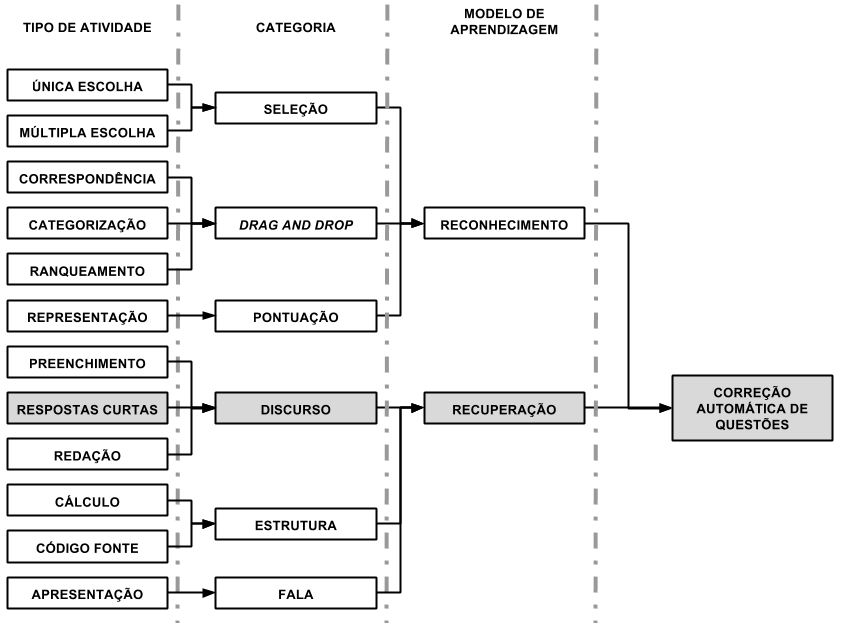
\includegraphics[width=\textwidth]{figuras/tiposAtividade}
\caption{A extração da informação e os tipos tradicionais de atividade aplicadas no cotidiano de sala de aula.}
\label{fig-atividades}
\end{figure}

Como apresentado na Figura \ref{fig-atividades} o professor dispõe de alguns modelos de atividades que, refletem diferentes aspectos do aprendizado. Temos quesões que são abertas e com pouca ou nenhuma restrição como as redações \cite{almeida-junior2017} ou respostas fechadas para uma única palavra, elencadas como opções no enunciado. As respostas discursivas encontram-se em âmbito intermediário \cite{bailey2008}. As respostas curtas, por sua essência, visam estabelecer a relação entre o conhecimento do aluno e o conteúdo encontrado no material didático. A Figura \ref{fig-SAG-concepts} demonstra como o espectro de questões trabalhados através das respostas discursivas curtas \cite{spalenza2017}.

\begin{figure}[!h]
\centering
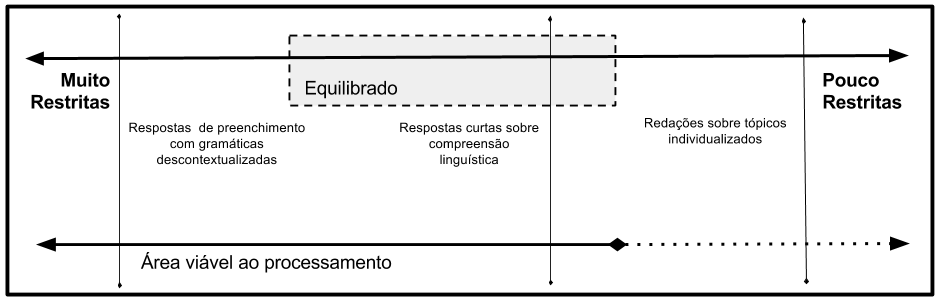
\includegraphics[width=\textwidth]{figuras/aprendizadoSAG}
\caption{Extração de informação em questões discursivas: entre respostas pequenas não-convergentes e a subjetividade das competências na avaliação de redações.}
\label{fig-SAG-concepts}
\end{figure}

A Figura \ref{fig-SAG-concepts} posiciona as respostas curtas enquanto um nicho das questões discursivas. O ideal é que, dentre os conhecimentos, a questão deve evitar abordar temas de cunho interpretativo ou temas individuais, que tangenciam experiências específicas de cada aluno \cite{siddiqi2008}. A representação da resposta deve ser completa, com a resposta dando embasamento para a correção, evitando informações restritas ou codificadas \cite{ding2020}. O enunciado deve guiar o aluno, de forma que as respostas sejam convergentes \cite{suzen2020, filighera2020}. Para isso, é fundamental que o sistema realize ao menos três etapas. A primeira etapa é o aprendizado do modelo de respostas do aluno \cite{ramachandran2015b}. A segunda etapa é reconhecer o padrão avaliativo do professor através do modelo de respostas \cite{funayama2020}. A terceira etapa é replicar o modelo avaliativo e elaborar \textit{feedbacks} coerentes \cite{fowler2021}.


\section{\textit{Active Learning}}

Em ML, o aprendizado é formação de conhecimentos a partir de dados através da interpretação dos padrões \cite{bishop2006}. Esse procedimento que dita a forma de aquisição de informações do sistema para criação de modelos com desempenho similar ao humano. Neste trabalho apresentamos um método de amostragem por \textit{Active Learning} \cite{kumar2020}, com anotação iterativa do professor em itens selecionados através das etapas de clusterização \cite{horbach2018}. Presente uma série de sistemas SAG \cite{basu2013, zhang2016, marvaniya2018}, as técnicas de clusterização utilizam \textit{Unsupervised Learning} para avaliação com base na similaridade das amostras. Porém, os trabalhos geralmente utilizam \textit{Supervised Learning}, criando modelos através de amostras da avaliação do especialista.

Portanto, a grande maioria dos estudos utiliza o particionamento entre treino e teste dos dados, previamente selecionado nos \textit{datasets}. Considerando cada resposta dos estudantes uma amostra, o particionamento em treino e teste reflete a divisão \textit{a priori} do conjunto de dados em um grupo para criação do modelo e outro para avaliação \cite{heilman2015}. Esse formato clássico permite ao sistema observar apenas uma parcela dos dados para reconhecimento dos padrões, realizando a inferência nas demais amostras até o momento desconhecidas \cite{bishop2006}. Assim, esses sistemas utilizam um conjunto de treino para extração do critério avaliativo, treinando o modelo para replicar o método de atribuição de notas, pressupondo a equivalência dos mesmos.

Portanto, o conjunto de amostras entre treino e teste não é necessariamente o mesmo. Por conta dessa divegência, essa técnica de aprendizado não refletem completamente o uso do professor com um sistema SAG \cite{sung2019a}. Uma atividade avaliada com um modelo SAG pode ser utilizada para uma série de aplicações, em um diferente momento e com outro grupo de estudantes. Portanto, com uma nova iteração, outros tópicos podem ser levantados em cada resposta. A tendência nesses casos é a avaliação incorreta de parte dos dados por conta da rigidez do conjunto fixado para o treinamento.

Outros métodos utilizam apenas alguns exemplo de resposta alvo, deniminadas respostas candidatas \cite{banjade2015, roy2016}. As respostas candidatas, são amostras elaboradas pelo professor e anotadas para representar seus padrões avaliativos. Os sistemas SAG com base nesse tipo de dado buscam, em geral, a comparação direta entre as respostas e o índice de sobreposição \cite{kar2017, jimenez2013}. Porém, este tipo de treinamento gera uma tendência na avaliação, com limitações na capacidade do modelo interpretar o conteúdo das respostas dos alunos \cite{ramachandran2015a}. As limitações da informação passada são um contraponto à liberdade textual das questões discursivas curtas. Além de tornar-se engessada, a resposta candidata também não garante o alinhamento para os demais documentos do \textit{dataset}.

Para contornar parcialmente essas limitações, ainda existem alguns métodos que utilizam mais informações sobre a atividade na etapa de treinamento, como o enunciado, o material de apoio e o quadro de \textit{rubrics}\cite{ramachandran2015b, wang2019}. O enunciado e o material de apoio adicionam ao sistema conhecimento externo sobre o tema. Enquanto as respostas candidatas e o quadro de \textit{rubrics} são materiais descritivos do modelo avaliativo do professor para todos, inclusive o sistema \cite{mizumoto2019, marvaniya2018}. Por outro lado, existem sistemas que demandam modelos mais complexos do método avaliativo, como regras de avaliação e filtros de conteúdo feitos manualmente \cite{pribadi2017, butcher2010}.

Outra estratégia é o uso de \textit{Data Augmentation}. Com \textit{Data Augmentation} as amostras passadas como treinamento são combinadas para representar de forma mais complexa o modelo avaliativo. O uso do aumento de dados torna os sistemas tradicionais um pouco mais robustos a alterações e mudanças nos padrões básicos, reduzindo a ocorrência de classificações tendenciosas \cite{kumar2019, lun2020}. Assim, a quantidade de amostras para treinamento e variações para cada modelo de resposta torna-se muito superior à quantidade dada inicialmente.

De forma diferente das estratégias citadas, o método de \textit{Active Learning} prioriza a identificação das principais amostras para otimização do esforço de anotação \cite{kumar2020}. A proposta combina os métodos de \textit{clusterização} e classificação \cite{oliveira2014} para identificar em cada iteração os diferentes tópicos abordados nas respostas. Assim, a evolução do conjunto de dados acontece durante cada uma das iterações. A clusterização, via \textit{Unsupervised Learning}, não recebe dados anotados e extrai as respostas distintas com base no nível de similaridade \cite{everitt2011}. E a classificação, via \textit{Supervised Learning}, coleta as anotações do especialista nas amostras selecionadas para treinamento do modelo \cite{bishop2006}. A partir daí que o modelo treinado replica a avaliação para as demais respostas.


\section{Classificação de Documentos}

A classificação de documentos, tradicional área de ML, possui inúmeras subdivisões segundo a especialização, motivação e conteúdo do conjunto de documentos. As referências a cada conjunto de documentos podem ser dadas também como \textit{dataset}, base de dados ou \textit{corpus}. A coleção destes, porém, é denominada \textit{corpora}. A classificação de documentos envolve treinar algoritmos de classificação com exemplos rotulados para replicar métodos de identificação de conteúdo e rotulação feitos por um especialista \cite{baeza2011}. Portanto, para além da origem e conteúdo dos documentos, o algoritmo deve se adaptar para especialização na triagem dos documentos de acordo com suas características.

O especilista realiza uma leitura dos documentos e identifica informações específicas que justificam a categoria atribuída. Para replicar tal tarefa, através da análise do conteúdo, o sistema deve identificar características que estão diretamente relacionadas a cada classe de documentos. Dependendo da característica dos documentos, o conteúdo relevante de um documento para categorização pode incluir a identificação de poucas palavras-chave até a formação de modelos linguísticos complexos \cite{jurafsky2009}. Por exemplo, na triagem de documentos pré-formatados as informações básicas como título, autor e organizações ou setores responsáveis podem ser descritores diretos da classe a ser atribuída. Por outro lado, em modelos como SAG, é necessário que relações textuais complexas sejam avaliadas para atribuição de notas \cite{paiva2012, yang2021}.

Deste modo, a atribuição de notas torna dos sistemas SAG uma complexa tarefa de classificação de documentos. É essencial a adaptação do algoritmo de acordo com o método de classificação utilizado pelo especialista. Portanto, apesar do conteúdo textual, a subjetividade do critério de avaliação deve ser levada em consideração pelo sistema \cite{pado2021}. Assim, a combinação entre o reconhecimento do modelo avaliativo e o reconhecimento do modelo textual deve atender às expectativas do professor \cite{condor2020}. Enquanto em parte das situações as notas fortemente correlacionadas com a ocorrência dos termos, em outras o critério do professor pode ter baixa correlação com os termos e apresentar diferentes nuances na atribuição de notas \cite{azad2020}. Deste modo, é determinante que o sistema compreenda a essência do conteúdo do documento enviado por cada aluno para reconhecimento da relação com as respectivas notas atribuídas \cite{mohler2011}.

\section{Processamento de Linguagem Natural}

Para criação de um modelo linguístico, os sistemas utilizam estratégias de aquisição de informação com técnicas de NLP. As primeiras técnicas de SAG da literatura e os primeiros sistemas propostos utilizavam descritores \cite{galhardi2018a}. Os descritores são caracteríticas simples extraídas segundo o formato da escrita de cada documento. Em geral, são formados por características pré-definidas, de acordo com a estrutura da resposta do aluno, sem levar em consideração a profundidade do conteúdo \cite{mohler2009}. Dentre os descritores, os mais comuns eram a contagem de erros da linguagem, a quantidade de palavras e a frequência de certas classes gramaticais \cite{riordan2019, galhardi2018b}. Porém, as características pré-definidas, consequentemente, não atendem a uma grande quantidade de respostas, criando modelos linguísticos com pouca aderência ao conteúdo.

Posteriormente, observando os diferentes propósitos das questões discursivas curtas e sua aplicação multidiciplinar, surgiram estruturas para maior aquisição de informação e modelagem linguística \cite{kumar2019, saha2018}. Os modelos linguísticos ampliaram a aderência do sistema ao tema das atividades. Assim, através do conjunto de respostas, cada sistema elabora modelos linguísticos com contexto suficiente para encontrar associações entre palavras \cite{tan2020}. Através dessas associações, os sistemas estabeleceram relações complexas entre os termos de cada resposta e o método de atribuição de nota do professor \cite{sahu2020}.

As estratégias voltadas na análise do texto por completo, adicionaram muita informação aos sistemas. Porém, tais informações não necessáriamente são relevantes para o método avaliativo. Como consequência, ocorreu a evolução, desenvolvimento e uso de técnicas de ponderação, seleção de características e identificação de padrões textuais \cite{banjade2016}. Para ponderação textual o modelo mais comum é o Term Frequency - Inverse Document Frequency (TF-IDF) \cite{baeza2011}. O TF-IDF é um método clássico que realiza a ponderação de acordo com a frequência dos termos, equilibrando a relevância de cada termo segundo sua ocorrência nos documentos e no \textit{dataset} \cite{sultan2016}. Por outro lado, dentre as técnicas de seleção de características que se destacam, o \textit{Latent Semantic Analysis} (LSA) \cite{landauer1998} é uma das mais utilizadas na literatura \cite{basu2013, sahu2020}. O uso desta técnica compreende identificar relações semânticas dentro do conjunto de respostas \cite{mohler2009}. Assim, através do LSA, os sistemas reunem o conteúdo que potencialmente contém maior significância no tema.

Entretanto, os modelos linguísticos criados através da frequência dos termos de cada resposta dos estudantes ainda não refletem uma análise complexa tal qual a do especialista. Portanto, na literatura existem estudos que propõe maior extração de informação textual, ainda que em textos curtos, para formação de componentes linguísticos mais robustos \cite{saha2018, zesch2018}. Uma estratégia é a análise estrutural dos termos, observando a construção frasal de cada resposta de aluno. Deste modo, na literatura alguns trabalhos citam a análise da construção gramatical das sentenças \cite{ramachandran2015b, roy2016}.

Outras propostas porém, remontam o contéudo das respostas sob a perspectiva sequencial da construção textual \cite{kumar2017}. A análise, com a seleção de \textit{n} termos de cada sentença da resposta é denominada \textit{n-grams} \cite{manning1999}. Os sistemas avaliam as respostas através da vetorização das respostas com análise de compatibilidade entre essas sequências \cite{sakaguchi2015, sultan2016}. Essas sequências subdividem cada resposta em pequenos trechos que contém de 1 a \textit{n} termos para aplicar na análise de equivalência e sobreposição entre respostas \cite{jimenez2013}. 

Ainda nestes modelos, destacam-se propostas de seleção de características e filtragem de conteúdo \cite{higgins2014, spalenza2016a}. Para filtragem de conteúdo, a identificação de termos comuns ou de baixa frequência representam um refinamento no modelo para análises mais consistentes do conteúdo \cite{zhang2020, marvaniya2018}. Termos comuns da linguagem em geral podem ser encontrados como \textit{stopwords}, organizados em listas, são conectivos linguísticos muito utilizados que não têm aderência ao tema \cite{jurafsky2009}. Entretanto, em situação oposta, palavras com baixa frequência, com uso específico e, em geral, não são fundamentais para a resposta do aluno. Em ambos os casos, a filtragem propõe que termos de baixa correlação com o tema sejam removidos. Com uma proposta diferente, a seleção de características interpreta o conjunto de documentos em busca de termos correlatos. De acordo com a frequência de ocorrência e associação dentro do conjunto de respostas, termos são selcionados visando ampliar a capacidade do modelo avaliativo \cite{krithika2015, spalenza2016b, horbach2018}. Portanto, o intúito da seleção de características é diretamente relacionado ao modelo linguístico e avaliativo da base de conhecimento. Nessa perspectiva, apenas os termos selecionados são utilizados para representar o conjunto de respostas.

Recentemente, algo um pouco mais robusto do que a análise de vizinhança de termos vêm sendo empregada para avaliar a linguagem segmentos de resposta. Para isso, cada termo é avaliado por similariade no contexto ao qual é empregado. Um método em especial aplicado nesta proposta é denominado \textit{word embeddings} \cite{sung2019b, ghavidel2020}. As \textit{embeddings} são modelos linguísticos de grande dimensionalidade adquiridos de uma coleção de documentos \cite{goldberg2017}. Esses modelos relacionam o emprego de cada par de termos encontrados em coleções de larga escala. Assim, os sistemas avaliam a correspondência do emprego dos termos em cada sequência de forma pareada. Deste modo, os sistemas avaliam proximidade entre diferentes termos, frases e contextos de uso para cada resposta dos estudantes \cite{riordan2017}.

\section{Avaliação de Questões Discursivas Curtas}

Os sistemas SAG para análise documental complexa são compostos por um conjunto de métodos que incluem a criação do modelo linguístico, organização do conhecimento e a identificação de características relevantes. Apesar disso, uma parte fundamental dos sistemas SAG são os classificadores de alta qualidade \cite{funayama2020}. Portanto, são os classificadores que destacam o conhecimento adquirido nas etapas anteriores e o apredizado do modelo avaliativo \cite{mohler2011}.

O propósito do classificador é compreender, replicar e descrever o modelo do professor (especialista) \cite{yang2021}. Assim, é função do sistema identificar caracerísticas relevantes para assimilar a forma que o professor avalia cada resposta enviada pelos estudantes \cite{jordan2012, mao2018}. Em geral, os avaliadores automáticos são divididos segundo quatro diferentes técnicas: por mapeamento de conceitos, extração de informação, análise de \textit{corpus}, algoritmos de ML \cite{burrows2015}. 

O método de mapeamento de conceitos consiste em um processo de detecção de determinado conteúdo nas respostas produzidas pelos estudantes. O reconhecimento de conteúdo, portanto, é realizado com análise de alinhamento entre termos de respostas \cite{jimenez2013}. Deste modo, é fundamental neste método avaliativo, identificar a existência dos principais conceitos nas respostas para a atribuição de notas \cite{kar2017, chakraborty2017}. Porém, mesmo com a construção automática de padrões através da amostragem, não é garantida a consistência dos modelos produzidos \cite{azad2020}. Deste modo, o principal fator destes sistemas é a busca por compatibilidade entre respostas, tornando o sistema muito dependente do objetivo da questão e o conteúdo enviado nas respostas \cite{filighera2020}.

Por outro lado, métodos de extração de informação apresentam características de identificação factual nas respostas dos estudantes. Portanto, compreendem métodos mais robustos de análise do conteúdo, sendo compostos por operações de reconhecimento de padrões e séries de expressões regulares \cite{ramachandran2015b, butcher2010}. Assim, sistemas SAG com base na extração de informação apresentam modelos de resposta para análise da equivalência de cada resposta com a expectativa de resposta do professor. Deste modo, a associação entre respostas estabelece maior profundidade ao conhecimento do sistema sobre o conteúdo \cite{tan2020}. Então, o modelo de avaliação utilizado pelo sistema torna-se próximo da observação do professor ao conjunto de respostas, porém, atendendo apenas modelos pré-definidos.

De forma distinta, os métodos baseados em \textit{corpus} traçam análises estatísticas das respostas de cada conjunto de dados \cite{kumar2019}. Neste método, os sistemas utilizam de análises da linguagem para validação do alinhamento entre respostas, interpretar variações de uso e caracterizar o conteúdo das respostas \cite{ziai2012, menini2019}. Para além dos termos utilizados, a adição de informação acrescenta diversidade semântica, tornando modelos mais flexíveis para análise do vocabulário do material \cite{fowler2021}.

Apesar da consistência dos modelos anteriores, existem limitações em um âmbito geral da aplicação de cada uma das técnicas de acordo com um base de conhecimento \cite{riordan2019, ding2020}. Em geral, as descrições de modelo avaliativo do especialista não representam bem o conhecimento para a criação do modelo avaliativo do sistema \cite{filighera2020}. Em contraste aos modelos superficiais, as técnicas de ML foram incorporadas na análise textual para criação de modelos mais robustos, com fundamentação estatística \cite{galhardi2018b}. Assim, modelos de aprendizado alinham o conteúdo dos documentos, através das diferentes componentes textuais, para reconhecimento dos padrões \cite{suzen2020}. Portanto, os métodos criam estruturas mais complexas que regras, sendo capazes de avaliar formatos distintos de resposta \cite{zhang2016, saha2019, camus2020}. A robustez destes modelos permite a associação de padrões não convergentes, podendo estabelecer critérios distintos para amostras atribuídas a uma mesma nota.

Em geral, um objetivo dos sistemas SAG, descrito pela literatura, é mesclar os métodos e suas dinâmicas de aprendizado para evolução do modelo avaliativo \cite{burrows2015, zesch2018}. Deste modo, é essencial a construção de modelos que comportem padrões avaliativos de alta qualidade e similares ao do especialista, reproduzindo com alta qualidade através de ML \cite{jordan2012}. Apesar das dificuldades e dos detalhes subjetivos da avaliação \cite{roy2018}, o intúito é que o desenvolvimento do modelo avaliativo compreenda a relação entre diferentes características de avaliação e a capacidade de atender diferentes domínios \cite{sung2019a, saha2019}. Portanto, espera-se o desenvolvimento de sistemas SAG mais robustos, lidando com diferentes combinações entre respostas e avaliações, aprendendo pela demanda do professor o domínio empregado.
% ==============================================================================
% Tese Marcos A. Spalenza
% Capítulo 3 - Proposta do Trabalho
% ==============================================================================
\chapter{Método}
\label{cap-metodo}

Neste trabalho, apresentamos o \textit{p}Nota, um SAG que aplica \textit{Active Learning} para análise da relação entre o conteúdo das respostas dos estudantes e o método avaliativo do professor. Acompanhando o desenvolvimento recente da literatura dos sistemas SAG \cite{burrows2015, bonthu2021, haller2022}, identificamos pontos sensíveis e problemas descritos nesses estudos. Utilizamos como base os fundamentos de análise documental e modelagem do método avaliativo do tutor para a criação de uma proposta SAG. Com esse direcionamento, é possível verificar os principais métodos para análise das componentes textuais para elaborar um conjunto robusto de informações sobre cada resposta. O conhecimento das respostas é vinculado ao critério de avaliação do professor. Com isso, espera-se construir modelos que maximizem os resultados na atribuição de notas, aproximando-se do formato de correções do especialista. A estrutura do \textit{p}Nota é particionada em módulos responsáveis por diferentes etapas do processo, como apresentado na Figura \ref{fig-esquema}.

\begin{figure}[!h]
\centering
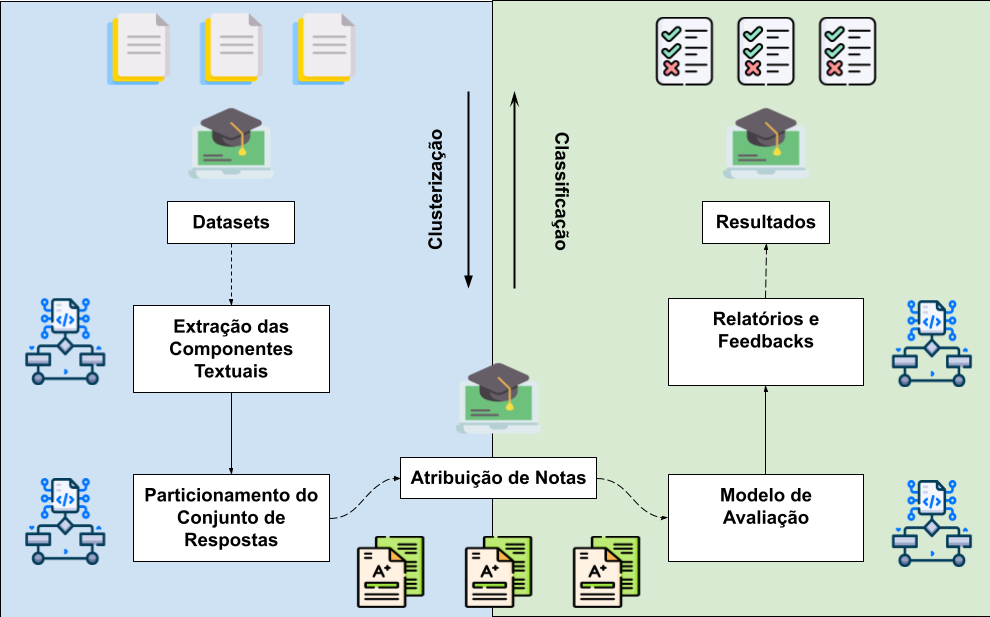
\includegraphics[width=\textwidth]{figuras/estrutura-pNota.png}
\caption{Esquema do \textit{p}Nota dividido em seus quatro módulos.}
\label{fig-esquema}
\end{figure}


Desse modo, tal qual ilustrado na Figura \ref{fig-esquema}, o sistema é composto por quatro módulos. Além destes, outros três processos dependem do estado do documento na avaliação. O primeiro módulo é a \textit{Extração das Componentes Textuais}, que realiza os ciclos de coleta de dados, verificação textual, extração da informação e organização do conhecimento. Nesse módulo o sistema analisa cada resposta com aplicação de tratamentos textuais para padronização e aquisição de conhecimento. O resultado dessa etapa é um conjunto de vetores de documentos com múltiplos níveis de análise da linguagem empregada.

O segundo módulo é composto pelas técnicas de \textit{Particionamento do Conjunto de Respostas}. Nesse núcleo são empregados métodos de otimização em \textit{clustering} para uma seleção representativa do conteúdo textual. Tais técnicas são descritas em detalhes na Seção \ref{sec-amostragem}. A representação criada pelas amostras é o que define o aprendizado do sistema. Por conta disso, as amostras são escolhidas pela sua distribuição espacial \cite{salton1975, baeza2011}, buscando incluir todos os tópicos abordados no tema da questão. Aqui, aplicam-se técnicas de otimização selecionando o agrupamento com melhor desempenho nos índices qualitativos. 

A próxima etapa recebe as atividades particionadas em \textit{clusters} e com a atribuição de notas nas amostras selecionadas. Neste terceiro módulo, com a construção dos \textit{Modelos Avaliativos}, é realizada a calibração dos classificadores e a atribuição das demais notas. A calibração dos algoritmos busca refinar o critério avaliativo para compreender qual é a relação entre os termos e a nota resultante. Ao fim dessa etapa, as notas geradas colaborativamente entre professor e sistema são encaminhadas aos alunos.

Quando os resultados estão prontos, o sistema atua na etapa de \textit{Relatórios e Feedbacks}. Nesse ponto, todas as notas já foram atribuídas e é possível atuar na transparência do modelo avaliativo. Assim, com o conjunto de informações utilizadas durante os processos, são produzidos relatórios e \textit{feedbacks} que descrevem as notas atribuídas e os resultados do \textit{dataset}. Por fim, os relatórios proporcionam acesso ao formato da amostragem, distribuição de notas, análise de desempenho e descrição dos padrões de resposta. 

Antes da execução do sistema, existe a aplicação em sala de aula. Por meio dos AVA, o \textit{p}Nota busca acompanhar a evolução das salas de aula digitais, com o \textit{Ensino a Distância} (EAD) e a disseminação dos MOOCs \cite{mohapatra2017}. Para isso, utiliza-se um \textit{framework} de coleta para transferência e controle das atividades da sala virtual para processamento externo \cite{spalenza2018}. Portanto são responsabilidades da aplicação a coleta das atividades no ambiente virtual, a transferência para um servidor de processamento e o envio de resultados para o professor. Na Figura \ref{fig-framework} é apresentado o funcionamento do método de coleta de dados em diferentes plataformas de ensino.

\begin{figure}[!h]
\centering
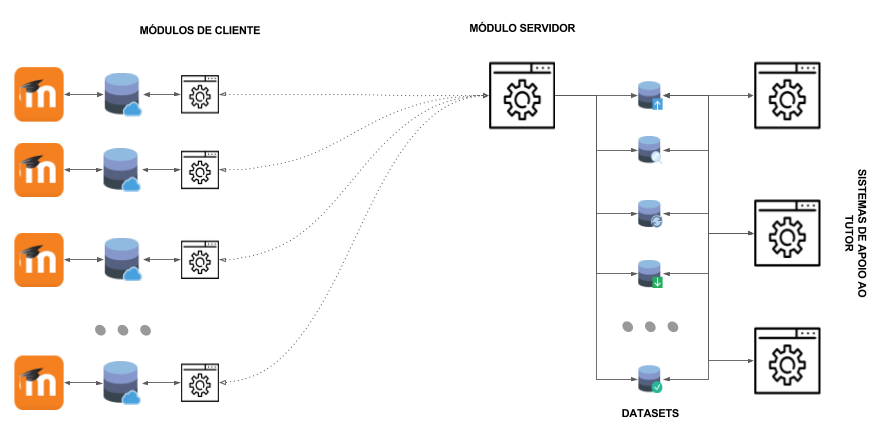
\includegraphics[width=\textwidth]{figuras/framework-moodle.png}
\caption{\textit{Framework} utilizado para transferência de dados, interligando plataformas AVA e o servidor do \textit{p}Nota.}
\label{fig-framework}
\end{figure}

Na Figura \ref{fig-framework} é apresentada a forma empregada na extração de informação dos AVA. Com a configuração, o módulo acessa cada cliente e transfere as atividades para o servidor de processamento do \textit{p}Nota. Então, o \textit{p}Nota solicita via AVA as requisições de avaliação e, após os resultados, também envia as notas para a plataforma. Adicionalmente, os \textit{feedbacks} gerados também são encaminhados individualmente a cada aluno. Na plataforma, após a apresentação das notas, o professor também pode realizar os ajustes necessários caso o resultado não esteja totalmente alinhado ao seu critério.

O professor, controla via plataforma o processamento, sendo aberto para determinar a finalização da atividade diretamente nela. O professor é livre para realizar alterações de qualquer nota mesmo que ainda esteja em análise pelo sistema. No controle do processo avaliativo, o professor fica responsável por monitorar a atribuição de notas e ajustar os resultados propostos pelo sistema.


\section{Extração das Componentes Textuais}
\label{sec-componentes-textuais}

A primeira etapa, \textit{Extração das Componentes Textuais}, realiza o carregamento e a análise do conteúdo textual. Inicialmente é realizada a leitura dos dados, carregando o conjunto de respostas que forma a atividade. É fundamental para extração que o arquivo seja recebido da forma como foi escrito pelo aluno na plataforma. Por conta disso, na sequência é realizada uma série de pré-processamentos que efetuam a limpeza destes documentos, com padronização, segmentação, filtragem, transformação e vetorização. O resultado após essa série de processos é a informação extraída, no formato de vetores com as componentes textuais de cada documento. Na Figura \ref{fig-ect} são apresentados os processos que compõem essa etapa.

\begin{figure}[!h]
\centering
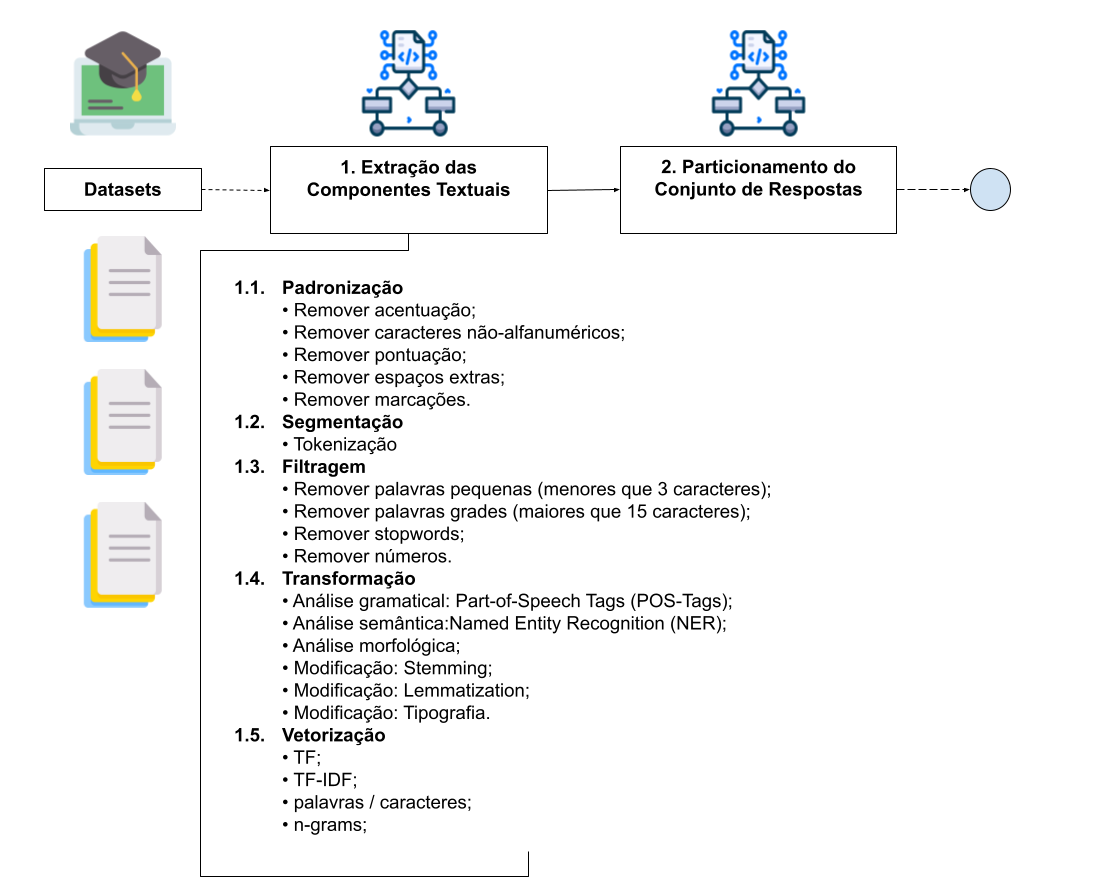
\includegraphics[width=\textwidth]{figuras/esquema-ect-pNota.png}
\caption{Detalhe do módulo de \textit{Extração das Componentes Textuais} no esquema do \textit{p}Nota.}
\label{fig-ect}
\end{figure}

Como é mostrado na Figura \ref{fig-ect}, realizamos todo o tratamento do texto nessa etapa, com coleta das informações. A padronização é composta pela coleta do conteúdo da resposta, remoção de dados não-informativos e aumento da equivalência entre as ocorrências dos termos. A segmentação efetua o particionamento das respostas em segmentos (\textit{tokens}) para verificação de cada termo. Com as frases particionadas, a filtragem seleciona as palavras com maior potencial de ter vínculo com o conteúdo. A transformação realiza análise do conteúdo para aquisição de informação em outros níveis de linguagem. Por fim, com documentos em padrões textuais realiza-se a vetorização, gerando vetores com cada \textit{token} ou série de \textit{tokens} representando o conteúdo enviado pelos alunos.

As respostas, que são recebidas em formato bruto, partem então para pré-processamentos e análises de conteúdo durante essa etapa. Aqui é fundamental a adição dos níveis de compreensão linguística, para amplificar a capacidade de aprendizado dos algoritmos nas próximas etapas. Assim, é pela forma que o texto é passado no formato vetorial \cite{baeza2011} que são identificadas respostas compatíveis até o passo da \textit{Avaliação}.


\subsection{Padronização}
\label{subsec-padronizacao}

% STD_MTH = ["accents", "punct", "spaces", "tags"]

Após o documento ser enviado pelo aluno, o conteúdo do(s) arquivo(s) está em estado bruto. No estado bruto, o conteúdo não segue padrões, em especial de codificação, espaçamento, acentuação e pontuação. É necessário portanto que o formato bruto chegue ao nível de escrita que o aluno enviou ao professor. Além disso, é fundamental remover conteúdos não interpretáveis, como caracteres não alfanuméricos e \textit{tags} (marcações). Portanto, essa etapa é composta pelos seguintes processos:

\begin{itemize}
	\item Remover acentuação;
	\item Remover caracteres não-alfanuméricos;
	\item Remover pontuação;
	\item Remover espaços extras;
	\item Remover marcações.
\end{itemize}

Após cada um dos passos, o texto do aluno está normalizado, tornando possível sua manipulação em nível de conteúdo. Pode-se inferir que a navegação no conteúdo só é possível após a remoção dos ruídos. São usados como exemplos as tags \textit{HTML} e a acentuação. Por um lado, os sinais da linguagem, como acentuação, são fundamentais para leitura e pronúncia dos termos. Mas estes são irrelevantes para identificação dos termos pelo sistema. Por outro lado, o inverso ocorre com marcações de arquivos textuais. São estruturas para leitura do sistema, mas não fazem parte do conteúdo produzido pelo estudante. Em ambos os casos, não existe qualquer relação desses dados com a semântica das respostas, e consequentemente, eles são removidos durante o processo. 

Os ruídos são muito comuns nos textos produzidos na internet, causados pela transferência de arquivos em repositórios externos, \textit{crawlers} ou \textit{web services} \cite{han2011}. Portanto, é a remoção de dados que aproxima a interpretação computacional proposta do envio do estudante na plataforma.

\subsection{Segmentação}
\label{subsec-segmentacao}

% TKN_MTH = ["simple", "word", "regex", "informal"]

Com os documentos passíveis de interpretação, e bem próximos ao que foi enviado pelo aluno, começa-se uma análise detalhada de seu conteúdo. Este é iniciado com o particionamento de cada texto em segmentos menores. A segmentação divide em menores componentes de resposta, seja por caracteres, frases ou parágrafos. Cada particionamento, no entanto, é apenas uma forma de entrada para os procedimentos realizados na sequência. Enquanto parte dos processos faz uso do texto em formato de segmentos de palavras, outros fazem análise contextual, comumente aplicada em formato de segmentos de frase.

É mais comum o formato de segmentos de palavras, denominados \textit{tokens}. Em todos os casos os segmentos são extraídos com base em uma \textit{heurística}, que delimita cada segmento. A \textit{heurística} mais comum para \textit{tokenização} é a divisão pelo espaçamento, eliminando os espaços em branco e considerando as palavras. Porém, esses métodos simples são sujeitos a muitas falhas. Nesses casos, são melhores os métodos construídos especificamente para a linguagem, considerando formas específicas de pontuação e divisões textuais. A \textit{tokenização}, então, é o método que transforma o conteúdo em uma lista de palavras.

A sequência de palavras permite que os próximos níveis trabalhem a perspectiva de cada \textit{token} dessa lista ou de sua vizinhança. Mesmo assim, é muito comum que, durante o processo, o documento seja manipulado de diferentes formas, inclusive passando várias vezes pela transformação de texto em lista de \textit{tokens} e vice-versa. Nesse formato, os \textit{tokens} permitem que haja navegação pelos termos adjacentes tal qual a análise dos termos de forma independente.


\subsection{Filtragem}
\label{subsec-filtragem}
% FLT_MTH = ["smallwords", "stopwords", "largewords", "numerals"]


A filtragem de conteúdo é uma componente muito importante desse processo. Apesar de ser uma etapa que causa perda na informação inicial dos \textit{sets} de resposta, a proposta é identificar \textit{features} que adicionam pouco ou nenhum dado relevante. É esperado, que a inerente perda de informação cause melhoria na consistência e na equivalência entre os documentos. Guiada pelo sistema, a limpeza representa itens que têm baixa correlação com o tema, não sendo componentes do núcleo das respostas. Assim, podemos incluir os seguintes componentes como parte desse processo:

\begin{itemize}
	\item Remover palavras pequenas (menores que três caracteres);
	\item Remover palavras grandes (maiores que 15 caracteres);
	\item Remover \textit{stopwords};
	\item Remover números.
\end{itemize}

Com a filtragem, busca-se uma avaliação fortemente ligada ao tema e o emprego contextualizado. É necessário remover os demais termos, que seriam de baixa significância, pouca capacidade de interpretação e menor relação com o que conteúdo. Esse é o caso das \textit{stopwords}. As \textit{stopwords} são palavras que são empregadas na linguagem como conectivos e não estão conectadas com o conteúdo passado. Elas são extremamente importantes para a nossa interpretação e reconhecimento de contexto, mas não adicionam informação quando empregadas. Assim, a lista de \textit{stopwords} é composta por palavras fundamentais para a linguagem durante a comunicação, mas sem potencial para a análise do contexto.

No caso do tamanho das palavras ainda há uma situação adicional para além da aderência ao tema. A filtragem garante que possíveis ruídos que escaparam dos processos anteriores sejam removidos. Casos específicos como caracteres isolados, links e problemas de segmentação na origem podem gerar ruídos ainda nessa parte. Inclusive, sem uma análise matemática complexa, a verificação numérica também entra em boa parte desses casos e pode ser incluída na filtragem. Mas é importante reconhecer os impactos quando os filtros são aplicados. O filtro numérico, por exemplo, afeta diretamente a capacidade de análise de conjuntos de respostas compostas por valores ou datas. 

Uma dificuldade, entretanto, é quantificar qual é o nível de filtragem desejável, balanceando a aquisição da informação. O ideal é que todos os processos de filtragem não causem impacto nos núcleos da resposta, que contêm os termos essenciais e fortemente vinculados ao tema. Nessa linha, em sua maioria, os casos de filtragem de algumas palavras específicas não impactam a forma e mantêm os termos com aderência ao tema.

Nessa etapa, os filtros de conteúdos são métodos de redução de ruído, responsáveis por discernir quais termos podem ser extraídos de cada item de resposta. Os ruídos podem causar a queda no desempenho do algoritmo da mesma forma ou pior do que a perda de informação causada na filtragem. Assim, o ruído em meio ao texto pode ser um grande problema para o sistema durante a interpretação do conhecimento. Com isso, esperamos que a filtragem auxilie os processos subsequentes com a capacidade interpretativa e relacional entre as respostas na formação do \textit{Modelo Avaliativo}.


\subsection{Transformação}
\label{subsec-transformacao}
% TRF_MTH = ["NER", "MORPH", "POS", "STEMM", "LEMMA"]

As análises de conteúdo são realizadas assim que os níveis anteriores prepararam o texto. Na transformação, a linguagem é analisada em níveis linguísticos. Neste processo, são interpretados alguns detalhes da construção textual para extração de \textit{features} via técnicas de NLP. Essas técnicas observam, entre as funções de cada palavra no texto, aspectos desde sua formação até sua função dentro da frase. Os diferentes níveis analisados nessa etapa são apresentados a seguir:

\begin{itemize}
	\item Modificação: Tipografia;
	\item Modificação: \textit{Stemming};
	\item Modificação: \textit{Lemmatization};
	\item Análise Gramatical: \textit{Part-of-Speech Tags} (POS-Tags);
	\item Análise Semântica:\textit{Named Entity Recognition} (NER);
	\item Análise Morfológica;
\end{itemize}

Cada uma das técnicas da lista aplica uma diferente transformação no texto. A primeira, bem simples, realiza a conversão do texto para uma tipografia comum, seja ela com letras maiúsculas ou minúsculas. Por outro lado, \textit{stemming} realiza conversão mais complexa, recuperando a raiz da palavra na construção da linguagem. Com \textit{stemming}, as palavras são convertidas para um núcleo comum, removendo as flexões, os prefixos e os sufixos. Por outro lado, um método equivalente é realizado com \textit{lemmatization}. Nesse outro, as palavras são convertidas para o \textit{lemma}, a palavra base, na forma com a qual é encontrada nos dicionários \cite{baeza2011}. 

Os métodos analíticos compõem ainda outras três formas mais robustas de identificação linguística. A técnica de \textit{POS-Tags} aplica a extração da função gramatical de cada palavra segundo seu emprego na frase. Em âmbito gramatical, identifica-se qual é o papel de cada palavra no contexto, entre verbos, adjetivos, pronomes, totalizando 17 categorias \cite{marneffe2021}.

Em nível semântico, aplica-se \textit{NER}, classificando o tipo de entidade nomeada de cada um dos \textit{tokens}. Com o NER, os nomes encontrados no texto são caracterizados pela classe que eles representam \cite{pirovani2019}. Entre as categorias reconhecidas há \textit{pessoa} (PER), \textit{local} (LOC), \textit{organização} (ORG) e \textit{diversos} (MISC). Isso permite que o sistema reconheça de forma simétrica diferentes menções dentro do conjunto de respostas para as principais categorias de entidades.

Por fim, o analisador morfológico identifica características da construção de cada palavra. Pela análise morfológica, as palavras são representadas pela sua flexão. Entre as flexões classificadas por cada termo estão as nominais (como gênero, número e definição) e verbais (pessoa, modo, tempo, voz). Além disso, esse mesmo processo também é responsável por algumas classificações léxicas de pronomes, adjetivos e advérbios \cite{marneffe2021}.

Cada uma dessas transformações é realizada para ampliar o conhecimento de cada \textit{token}. As análises mais complexas da linguagem e as categorizações dos termos permitem que as respostas sejam interpretadas de forma mais profunda. Essa profundidade é necessária para que, além do nível textual, a simetria das respostas seja levada em consideração. Desse modo, nesse ponto, a linguagem torna-se mais próxima da compreensão do algoritmo do que da forma original, aplicada na escrita.

A resultante desses processos é uma forte análise das componentes textuais de cada documento, buscando a identificação e a compreensão das estruturas textuais \cite{spalenza2020}. Com maior profundidade textual, espera-se tornar o sistema mais flexível para lidar com texto livre \cite{ding2020}. Assim, apesar das nuances da linguagem, o sistema consegue reconhecer e lidar com padrões que estão na composição de cada sentença \cite{filighera2020}. Então, a compreensão de diferentes níveis linguísticos é fundamental para a construção do SAG \cite{sahu2020}.


\subsection{Vetorização}
\label{subsec-vetorizacao}

A vetorização, como última etapa do pré-processamento, é responsável por extrair o modelo numérico de cada documento, permitindo mensurar a diferença ou a equivalência para os demais da coleção. Dessa forma, os documentos são representados por vetores numéricos segundo seu padrão de características. Cada uma das \textit{features} é analisada conforme sua frequência de ocorrência em cada documento do \textit{dataset}. A representação vetorial numérica de cada documento pela frequência é denominada \textit{Term Frequency} (TF). Sendo a coleção de documentos $ D = \{ d_{0}, d_{1}, d_{2}, \hdots d_{i} \} $ e as \textit{features} encontradas nos documentos $ F = \{ f_{0}, f_{1}, f_{2}, \hdots f_{j} \} $.  Portanto, para cada documento $ d $ na coleção $ D $, conta-se a frequência de cada \textit{feature} $ f_{j} $ do vocabulário $ F $. Assim, a forma vetorial do documento de índice $ i $ é dada por $ d_{i} $, sendo o vetor composto pela frequência $ n $ de cada \textit{feature} no documento $ n_{i, j} $. Então, cada documento é representado em $ D $ por sua forma vetorial $ d_{i} = [\ n_{i, 0}, n_{i, 1}, n_{i, 2} \hdots n_{i,j} ]\ $, usando TF.

Dadas as diferenças entre a frequência de cada termo em cada documento, é aplicada a ponderação para equilibrar a relação de frequência. A ponderação é denominada \textit{Inverse Document Frequency} (IDF). O \textit{Term Frequency-Inverse Document Frequency} (TF-IDF) estabelece a relação de que termos que ocorrem em muitos documentos têm menor relevância \cite{baeza2011}. A ponderação ocorre conforme a Equação \ref{eq-tfidf}.

\begin{equation}
TF-IDF = d_{i,j}* \log \frac{n_{D}}{n_{d_{j}}}
\label{eq-tfidf}
\end{equation}

O IDF é uma ponderação na frequência de cada \textit{feature} no vetor $ d_{i, j} $, segundo o total de documentos $ n_{d_{j}} $ que contém $ f_{j} $ em relação ao total de documentos da coleção $ D $. Essa ponderação reduz a diferença numérica entre uma \textit{feature} encontrada em todos os documentos para as \textit{features} que estão apenas em grupos específicos de documentos. Assim, o uso dessa forma potencialmente delimita melhores características (\textit{features}) para a construção de modelos avaliativos. A aplicação desse modelo está associada à capacidade de identificação de características com alta correlação a grupos específicos de nota.

No método de vetorização, durante a contagem de frequência de cada \textit{feature}, é priorizada a análise de vizinhança entre os termos. Preservando o aspecto textual, os \textit{n-grams} estabelecem a frequência conjunta dos termos dentro de sequências. Em vez de cada documento ser representado por um vetor simples da frequência de cada \textit{feature}, essa frequência é calculada segundo a sequências dos $ n $ termos. Sendo assim, aplicamos valores de $ n $ entre 1 a 5-\textit{grams}. São utilizadas simultaneamente as sequências de um a cinco termos, de forma a capturar o comportamento das estruturas textuais na formação dos documentos. Dessa forma, os padrões identificados em \textit{n-grams} \cite{spalenza2020} visam à associação entre \textit{features} fortemente correlacionadas nos vetores, compondo o modelo avaliativo.


\section{Particionamento do Conjunto de Respostas}
\label{sec-amostragem}

No formato vetorial, temos uma representação numérica dos documentos. Por meio dessa representação, podem ser comparadas as estruturas textuais que cada item de resposta contém. A comparabilidade permite identificar o comportamento das respostas definindo padrões. O conjunto desses padrões forma a distribuição das respostas no espaço vetorial. É possível assim, mensurar a proximidade entre as respostas, enquanto amostras, para formação de \textit{clusters} para análise. Aplicando \textit{Unsupervised Learning}, é realizado o \textit{Particionamento do Conjunto de Respostas} para identificar estruturas textuais similares e contextualizar as diferentes formas de resposta. Essa forma de extração de conhecimento por clusterização é apresentada na Figura \ref{fig-pcr}.

\begin{figure}[!h]
\centering
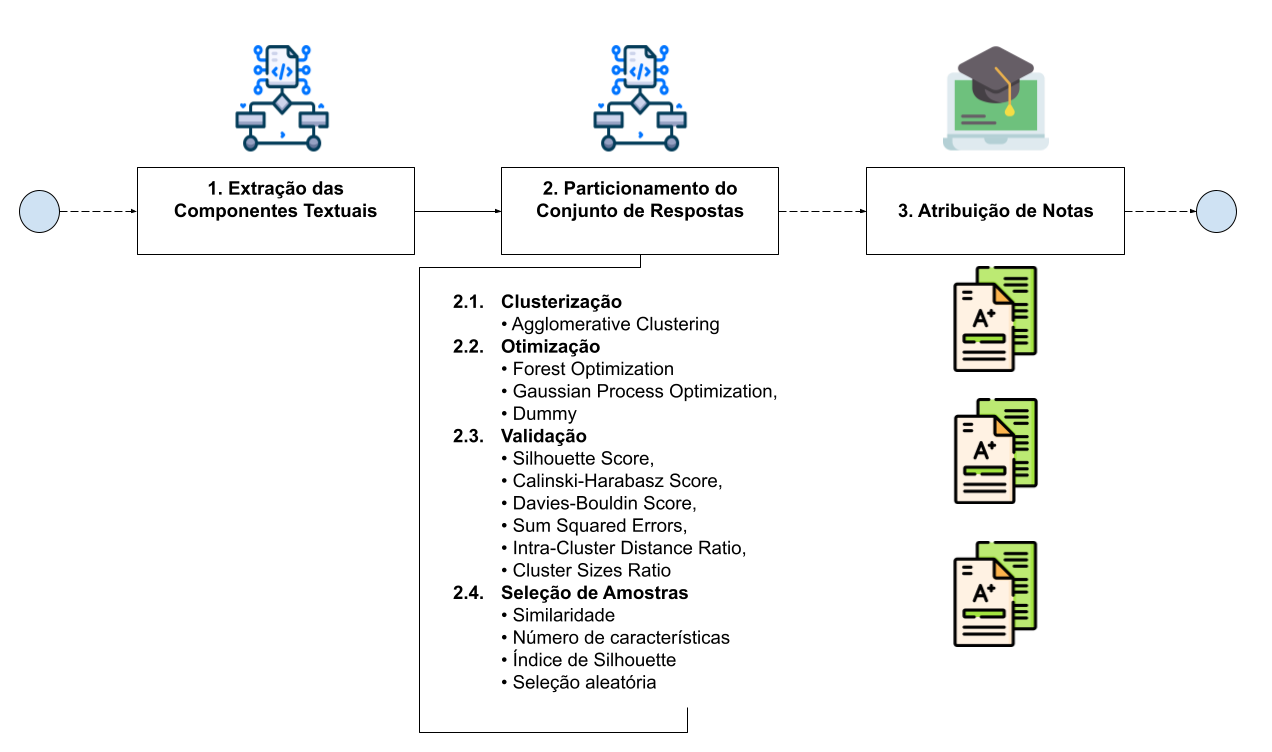
\includegraphics[width=\textwidth]{figuras/esquema-pcr-pNota.png}
\caption{Módulo de \textit{Particionamento do Conjunto de Respostas} no esquema do \textit{p}Nota.}
\label{fig-pcr}
\end{figure}

Na Figura \ref{fig-pcr} é apresentado um primeiro passo do método de \textit{Active Learning} empregado neste trabalho. São identificados diferentes componentes de resposta pela distribuição espacial dos vetores para anotação de amostras selecionadas do conjunto pelo especialista. A partir dessa forma de amostragem, são coletadas as notas, de acordo com o conteúdo que forma cada resposta ou grupo de respostas. Consequentemente, o processo de anotação requisitado pelo sistema vincula o conteúdo destas respostas com os padrões de avaliação do especialista. Diferentemente da maioria dos sistemas, que realizam amostragem aleatória, o \textit{p}Nota analisa as instâncias que compõem cada \textit{cluster} formado.


\subsection{Clusterização}
\label{subsec-clusterizacao}

É realizado o particionamento das respostas utilizando técnicas de clusterização. Esse processo é responsável por agrupar respostas em grupos por similaridade. O algoritmo de \textit{clusterização} utilizado é o \textit{Agglomerative} \cite{spalenza2019}, um método hierárquico de agrupamento por proximidade. O \textit{Agglomerative} compreende formar \textit{clusters} agrupando item a item até que um limiar de proximidade seja alcançado dado um $ k $ número de \textit{clusters} \cite{everitt2011}. Os grupos formados, ou \textit{clusters}, indicam algum nível de compatibilidade entre as estruturas que formam as respostas. Assim, a análise entre a equivalência e a divergência das respostas permite a contextualização da avaliação do especialista.

Para isso, precisamos que os \textit{clusters} sejam bons descritores do contexto, captando bem esse aspecto de equivalências e divergências textuais. A forma de designar se há o equilíbrio entre os \textit{clusters} foi realizada por meio do \textit{elbow method} \cite{everitt2011}. Esse método compreende testar uma sequência de parâmetros da clusterização para identificar a melhor combinação de \textit{clusters} formados segundo uma métrica de qualidade. Em geral, a métrica de qualidade é diretamente relacionada ao propósito de uso dos \textit{clusters}.

Entre as métricas estudadas estão \textit{Calinski-Harabasz Score} (CHS) \cite{calinskiharabasz1974}, \textit{Davies-Bouldin Score} (DBS) \cite{daviesbouldin1979}, \textit{Silhouette Score} (SS) \cite{rousseeuw1987}, \textit{Sum of Squared Errors} (SSE) \cite{maimon2005} e o \textit{Coeficiente de Variação} do tamanho do cluster (CVS). Essas métricas são denominadas \textit{Índices de Validação Interna} e avaliam os agrupamentos sem considerar a classe de cada amostra.

Cada índice é uma heurística utilizada para mensurar, sob diferentes perspectivas, a qualidade dos \textit{clusters} gerados em relação a outras formas de agrupamento de um mesmo \textit{dataset}. CHS mensura a razão entre a dispersão dos itens intra-\textit{cluster} e a dispersão extra-\textit{cluster}. DBS é o índice que estabelece a relação entre a média de similaridade entre as amostras do \textit{cluster} para a média de similaridade entre-\textit{clusters}. SS é a média entre as distâncias das amostras pertencentes a um \textit{cluster} em relação às amostras do \textit{cluster} mais próximo. SSE é uma métrica que avalia o erro de cada amostra que compõe um \textit{cluster} em relação ao seu centroide. O centroide é o ponto médio dos itens que constituem cada \textit{cluster}. Portanto, o centroide é uma instância representante da dispersão dos itens no \textit{cluster}, porém é um ponto artificial e não necessariamente uma amostra que o compõe. Por fim, CVS avalia o equilíbrio entre o número de amostras agrupadas em cada \textit{cluster}, considerando a diferença entre o maior grupo e o menor grupo formados.

Para a avaliação de respostas abertas, consideramos que o ideal são as análises que balanceiam os itens de cada \textit{cluster} em relação aos \textit{cluters} adjacentes. Por isso, \textit{clusters} com padrões muito específicos não devem formar bons descritores para a distribuição, mas sim para uma ou poucas amostras que compõe o grupo. Assim, para a proposta de \textit{Active Learning}, os grupos equilibrados têm maior potencial para aquisição de informação. Por outro lado, também é fundamental reconhecer a proximidade intra e inter-\textit{cluster}. Assim, foram combinados CVS e SS para avaliação amostral. Aplicamos CVS na formação dos agrupamentos enquanto o SS é observado durante a seleção amostral.


O processo de otimização, que incide sobre o \textit{elbow method}, testa os parâmetros de clusterização e visa reduzir o intervalo de busca enquanto maximiza os resultados do índice. Para isso, foram avaliados três métodos \textit{Forest Optimization}, \textit{Gaussian Process Optimization} e \textit{Dummy}. Os resultados obtidos com os dois primeiros foram equivalentes nesse contexto, sendo escolhido o \textit{Gaussian Process} para a aplicação \cite{spalenza2019}. Esse método analisa cada teste pela distribuição dos valores da métrica de qualidade como uma \textit{gaussiana}, buscando pontos de máxima da função. A resultante é dada pelo melhor valor encontrado. O parâmetro sob controle é o $ k $, número de \textit{clusters}. O intervalo de $ k $ é definido por valores de $ 2 $ até $ 2 * \sqrt{n} $, sendo $ n $ o número de amostras do \textit{dataset} \cite{han2011}. Simultaneamente, para cada combinação de $ k $ são testadas 20 métricas de distância.

\begin{itemize}
\begin{multicols}{4}
  \item braycurtis
  \item canberra
  \item chebyshev
  \item correlation
  \item cosine
  \item dice
  \item euclidean
  \item hamming
  \item haversine
  \item jaccard
  \item kulsinski
  \item mahalanobis
  \item manhattan
  \item matching
  \item minkowski
  \item rogerstanimoto
  \item russellrao
  \item sokalmichener
  \item sokalsneath
  \item yule
  \end{multicols}
\end{itemize}

O agrupamento selecionado é utilizado para amostragem em um percentual do conjunto de respostas disponíveis. Ainda avaliamos de forma qualitativa essa seleção segundo três índices \textit{Homogeneity} (HS), \textit{Completness} (CS) e \textit{Clustering Accuracy} (CA). Em uma ótica diferente da formação dos \textit{clusters}, com os índices qualitativos é mensurado o impacto de cada resultado da clusterização pela distribuição das classes. Esses são chamados \textit{Índices de Validação Externa}.

CA é o índice que avalia o desempenho da clusterização enquanto classificador por voto majoritário. Nesse cenário, cada \textit{cluster} é representado pela sua principal classe, mostrando a coesão dos grupos para sua representação de classe. Esse índice também estabelece um \textit{baseline} de desempenho de classificação. Essa métrica é simétrica a ACC, descrita na Equação \ref{eq-classification} da Seção \ref{subsec-classificacao}. HS é o índice que mensura se os \textit{clusters} são formados apenas por uma classe \cite{rosenberg2007}. CS por outro lado, avalia se todos os itens de uma classe estão presentes em um mesmo \textit{cluster} \cite{rosenberg2007}. Ambos são métricas que avaliam a entropia ($H$) dos \textit{clusters} dada a anotação das amostras, apresentadas na Equação \ref{eq-hs-cs}.

\begin{equation}
Homogeneity = 1 - \frac{H(y_{c} | \hat{y}_{c})}{H(y_{c})}
\label{eq-hs-cs}
\end{equation}

\begin{equation*}
Completness = 1 - \frac{H(y_{c} | \hat{y}_{c})}{H(\hat{y}_{c})}
\end{equation*}

A Equação \ref{eq-hs-cs} apresenta as métricas HS e CS, referências para a concentração das classes reais ($y_{c}$) dada a distribuição dos \textit{clusters} ($\hat{y}_{c}$). Assim, identifica-se o comportamento das classes de nota na distribuição pela entropia. Tais métricas permitem a identificação \textit{a posteriori} dos resultados mais coesos de clusterização. A concentração de classe por \textit{cluster}, permite uma melhor amostragem sendo possível amplificar os resultados obtidos na etapa de classificação.


\subsection{Seleção de Amostras}
\label{subsec-selecao-amostras}

Com a formação dos \textit{clusters}, identificam-se as principais respostas de cada agrupamento para inferência do modelo avaliativo do professor. A amostragem é realizada com a coleta de um percentual dos itens mais representativos que compõem o \textit{dataset}. Essa coleta analisa padrões de documentos de cada \textit{cluster}, a fim de compreender como é dada a avaliação do especialista para os diferentes padrões de resposta. As amostras são selecionadas conforme critérios específicos, descrevendo componentes do \textit{cluster}. 

A nossa amostragem segue alguns critérios. Os critérios definem a sequência de seleção para atingir o percentual escolhido para anotação. No primeiro grupo de amostras são selecionados os pares de amostras que apresentam maior e menor similaridade de cada \textit{cluster}. O segundo grupo é composto por amostras com mais e menos características. O terceiro grupo é formado de duas formas: pelo coeficiente \textit{silhouette} \cite{rousseeuw1987} de cada amostra ou pela seleção aleatória.

Nesse último grupo a análise de dispersão calcula o coeficiente de \textit{silhouette} da amostra. Tal qual o SS, esse índice determina a razão entre a distância da amostra para os demais itens do grupo em relação aos itens do \textit{cluster} mais próximo. Dessa forma, por meio desse método é incrementado o número de amostras por dispersão até alcançar o percentual de amostragem selecionado. Uma outra opção de seleção é a escolha de amostras pelo balanceamento do tamanho dos \textit{clusters}. Nesse caso, o método determina que um item seja aleatoriamente selecionado, ponderado de acordo com a quantidade de itens que compõem cada grupo. Descartando as duas opções anteriores, as amostras são selecionadas aleatoriamente entre todo o \textit{dataset}.

Terminando esse procedimento de seleção, as amostras são enviadas para atribuição de notas pelo professor. Na plataforma de correção que o professor adotou, ele realiza a atribuição de notas para cada item sugerido pelo sistema após a amostragem. Finalizado esse processo, com o conjunto de respostas representativas e suas respectivas notas atribuídas pelo professor, começa-se a análise de padrões para inferência das notas para as demais respostas.

\section{Modelo Avaliativo}
\label{sec-avaliacao}

O passo posterior à atribuição de notas, etapa com participação do professor, é a criação dos modelos computacionais. O \textit{Modelo Avaliativo}, é a etapa do \textit{p}Nota que desenvolve o SAG para replicar a forma de avaliação do professor. Assim, após a atribuição de notas, são criados os padrões que vinculam o texto e a avaliação.  O sistema, portanto, deve se aproximar da forma como o professor gera avaliações. A plataforma utilizada para reconhecimento de padrões de nota é apresentada na Figura \ref{fig-ma}.

\begin{figure}[!h]
\centering
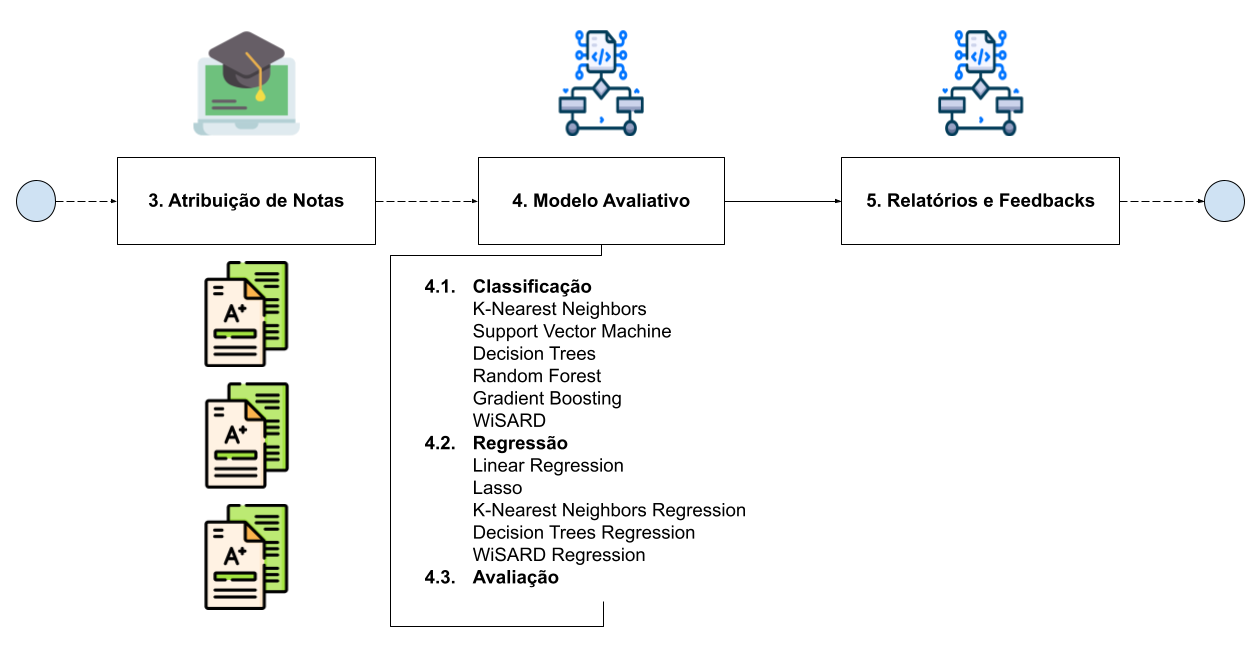
\includegraphics[width=\textwidth]{figuras/esquema-ma-pNota.png}
\caption{Etapa de construção do \textit{Modelo Avaliativo} no esquema do \textit{p}Nota.}
\label{fig-ma}
\end{figure}

Ao receber todas as notas para as amostras, o processo começa a construção dos modelos, tal qual ilustrado na Figura \ref{fig-ma}. A criação de um modelo SAG complexo compreende identificar detalhes correspondentes entre as respostas. O \textit{p}Nota analisa a correspondência entre notas e \textit{features} textuais para analisar equivalência. É possível considerar que padrões equivalentes de uma mesma nota têm alta probabilidade de serem relacionados ao que o professor considerou para avaliação. Cada atividade tem especificamente uma forma de avaliação e um padrão avaliativo alinhado com a prática do professor. Portanto, a identificação do critério avaliativo não é trivial. Por isso, a técnica de \textit{Active Learning} proposta neste estudo é fundamental para compreender o modelo e a forma que o professor trabalha durante a avaliação.

O \textit{Modelo Avaliativo} gerado pelo \textit{p}Nota é responsável por atender a expectativa de nota do professor. Sua função é vincular o padrão avaliativo com o padrão textual (\textit{features}) do conjunto de resposta. Então, a função da técnica de \textit{Active Learning} proposta é treinar classificadores contextuais, transformando os métodos tradicionais de ML em avaliadores especializados. Por meio do conhecimento de uma série de níveis de linguagem e da otimização da seleção de amostras busca-se reduzir os problemas que são incorretamente atribuídos apenas à técnica aplicada na atribuição de notas. Desta forma, espera-se que os \textit{Modelos Avaliativos} lidem com a variação linguística, a individualidade dos \textit{outliers} e o desbalanceamento dos níveis de nota.


\subsection{Classificação}
\label{subsec-classificacao}

O processo de classificação é utilizado em dois tipos distintos de avaliação: com notas ordinais e discretas. As notas ordinais permitem estabelecer ordem de escala numérica enquanto as discretas são textuais e requerem interpretação. No entanto, aos classificadores empregados, trabalha-se com a relação de diferença entre os níveis para aprendizado de convergência e divergência. Por um lado, a convergência indica equivalência entre os padrões de avaliação e texto encontrados nas amostras. Por outro lado, a divergência indica os padrões incompatíveis de texto por nota e entre níveis de nota, degradando sua influência avaliativa. As técnicas empregadas, em sua essência, devem assimilar o que compõe um nível de nota (equivalência) e o que é informação irrelevante ou auxiliar (divergência). Para estudar esses aspectos são aplicadas cinco diferentes formas de reconhecimento de padrões por meio dos algoritmos: \textit{K-Nearest Neighbors}, \textit{Decision Tree}, \textit{Support Vector Machine}, \textit{Gradient Boosting}, \textit{Random Forest} e \textit{WiSARD}.

O \textit{K-Nearest Neighbors} (KNN) é o algoritmo de classificação pela análise da vizinhança amostral. No KNN, cada amostra é categorizada pela distribuição local dos seus $ k $ vizinhos. A atribuição do rótulo é por voto majoritário, atribuindo o mesmo valor à amostra não anotada. Diferentemente deste, o algoritmo \textit{Decision Tree} (DTR) estabelece a equivalência entre amostras, sob uma perspectiva das características que as compõem. O DTR associa os grupos anotados com a mesma classe pelos limiar das características, gerando regras de decisão. As regras, elaboradas automaticamente, delimitam as principais \textit{features} segundo os valores de tendência de classe. O processo de classificação, então, acontece com a comparação de cada um dos itens dentre a cadeia de decisões na estrutura de árvore.

Outro tradicional algoritmo, o \textit{Support Vector Machine} (SVM) estabelece uma forma distinta de observar os dados. Os dados, em grupos por categoria, formam um \textit{kernel}. O \textit{kernel}, diferentemente do DTR, cria modelo espacial que delimita a diferença entre categorias. Então, cada amostra, é identificada segundo sua posição em relação ao limiar de características dado o modelo representante da classe. De forma similar é aplicado o algoritmo \textit{Wilkes, Stonham and Aleksander Recognition Device} (WSD) \cite{aleksander1984, wisard2020}, conhecido como \textit{WiSARD}\footnote{wisardpkg - https://github.com/IAZero/wisardpkg}. O algoritmo produz um modelo binário com o registro de padrões de características. Cada padrão é reconhecido em análise sequencial de um intervalo de bits predefinido. O modelo binário criado é comparado com as respostas não avaliadas, categorizando-as pela similaridade entre padrões. Especificamente para esse algoritmo, a conversão dos vetores TF-IDF em seu formato binário foi dada com 1 \textit{bit} por característica, de acordo com a esparsidade observada em dados textuais \cite{manning1999}. Assim, dado como pré-requisito de sua aplicação, o padrão submetido é dado pela existência (valor 1) ou não (valor 0) de cada característica na resposta.

Adicionalmente, dois modelos de \textit{ensemble} foram aplicados. Os \textit{ensembles} são técnicas que combinam vários classificadores mais simples para determinar áreas de decisão mais robustas. Os classificadores simples são denominados \textit{weak learners}, em busca de detalhes na avaliação entre termos e classes. Nesse aspecto, \textit{Random Forest} (RDF) é um algoritmo que combina o método tradicional \textit{Decision Tree} com \textit{subsets} de amostras. Desta forma, o RDF combina análises parciais do conjunto de dados para definir regras de decisão mais complexas sobre a distribuição de amostras. De modo similar, o \textit{Gradient Boosting} (GBC) combina uma série de \textit{Regression Trees} para otimização diferencial da função de perda (\textit{loss}). Nessa linha, o GBC observa o gradiente da função de perda com \textit{Logistic Regression}. Nesse aspecto, com uma série de amostragens, a técnica procura minorar o erro de classificação obtido com a calibração do modelo segundo uma sequência de \textit{subsets}. 

A combinação com modelos tradicionais e técnicas de \textit{ensemble} visa potencializar a capacidade analítica do método. Com diferentes formatos de dados, a proposta deste trabalho testa diferentes modelos procurando o que melhor se adapta ao padrão avaliativo do professor. Nesse aspecto, o método de classificação é escolhido de acordo com a similaridade entre o modelo automático com o critério do professor \cite{pado2021}. Para avaliar esse aspecto utiliza-se o coeficiente \textit{kappa} quadrático \cite{cohen1960}. As amostras são separadas em dois grupos acordo com o \textit{Stratified K-Fold}, para mensurar a capacidade de cada algoritmo na categorização das amostras. Dentro do próprio conjunto utilizado para treinamento dos modelos SAG, é possível avaliar a paridade dos resultados com o avaliador humano \cite{artstein2008}.

Na sequência, a qualidade de cada um é avaliada com quatro métricas. A \textit{Accuracy} (ACC), ou acurácia, mensura a equivalência percentual entre as avaliações. A \textit{Precision} (PRE), ou precisão, quantifica a atribuição correta de rótulos em razão da quantidade de atribuições incoerentes da mesma categoria. De forma similar, a \textit{Recall} (REC), ou revocação, quantifica a atribuição correta de rótulos em razão dos itens de determinada classe que foram classificados de forma incorreta. Por fim, F1 é o balanceamento entre PRE e REC, observando simultaneamente os erros de e para cada classe. A Equação \ref{eq-classification} apresenta a fórmula de cada uma das métricas citadas para avaliação qualitativa dos algoritmos de classificação testados.

\begin{equation}
Accuracy = \frac{TP+TN}{TP+TN+FP+FN}
\label{eq-classification}
\end{equation}

\begin{equation*}
Precision = \frac{TP}{TP+FP}
\end{equation*}

\begin{equation*}
Recall = \frac{TP}{TP+FN}
\end{equation*}

\begin{equation*}
F{1} = \frac{2*Precision*Recall}{Precision+Recall}
\end{equation*}

Na Equação \ref{eq-classification}, é possível observar as fórmulas para mensurar a qualidade dos classificadores. Nelas $ T $ refere-se aos casos verdadeiros e $ F $ aos falsos. Da mesma forma, $ P $ refere-se aos casos positivos e $ N $ aos negativos \cite{manning2008}. Porém, tradicionalmente a avaliação tem nuances que se extendem para além das marcações entre certo (ou verdadeiro) e errado (ou falso). Assim, as métricas são balanceadas conforme o número de classes, como determinado na Equação \ref{eq-classification-nlabels}. 

\begin{equation}
Accuracy = \frac{1}{n_\text{amostras}} \sum_{i=0}^{n_\text{amostras}-1} 1(\hat{y}_i = y_i)
\label{eq-classification-nlabels}
\end{equation}

\begin{equation*}
Precision_{macro} = \frac{1}{\left|n_{classes}\right|} \sum_{c \in n_{classes}} Precision(y_c, \hat{y}_c)
\end{equation*}

\begin{equation*}
Recall_{macro} = \frac{1}{\left|n_{classes}\right|} \sum_{c \in n_{classes}} Recall(y_c, \hat{y}_c)
\end{equation*}

\begin{equation*}
F{1}_{macro} = \frac{1}{\left|n_{classes}\right|} \sum_{c \in n_{classes}} F{1}_\beta(y_c, \hat{y}_c)
\end{equation*}

\begin{equation*}
F{1}_{ponderado} = \frac{1}{\sum_{c \in n_{classes}} \left|y_c\right|} \sum_{c \in n_{classes}} \left|y_c\right| F{1}(y_c, \hat{y}_c)
\end{equation*}

A Equação \ref{eq-classification-nlabels} mostra as métricas qualitativas aplicadas em avaliações com múltiplos níveis de nota, sendo $y$ o valor de nota atribuído para cada amostra ou grupo de amostras ($c$) \cite{manning2008}. Por definição, os SAGs são majoritariamente criados para avaliações com mais de uma classe de nota. É usada para mensurar o desempenho a média (macro) da atribuição de notas. Porém, pelo já esperado desbalanceamento entre notas, também avalia-se o F1 ponderado pela quantidade de amostras por classe. Comparando estatisticamente os desempenhos, via \textit{kappa}, a expectativa é selecionar o que tem notas mais adequadas ao modelo avaliativo do professor. Mas, o melhor modelo é o que efetivamente apresenta maior ganho de qualidade nessas métricas quando comparado com a avaliação final do professor.


\subsection{Regressão}
\label{subsec-regressao}

Outra forma de atribuição de nota é a não-categórica. Nesses casos, são chamadas de notas contínuas, pois apresentam um intervalo de notas possíveis mas sem níveis específicos. São aplicados os métodos de regressão, estimando a nota pela similaridade entre respostas. Nesse formato ainda se enquadram as noções de \textit{equivalência} e \textit{divergência} entre as \textit{features} das respostas na avaliação. Os cinco métodos de regressão aplicados são \textit{Regressão Linear}, \textit{Lasso}, \textit{K-Nearest Neighbors}, \textit{Decision Tree} e \textit{WiSARD}.

A Regressão Linear (LNRG) é um algoritmo que avalia a tendência linear das amostras segundo sua distribuição. Essa tendência linear busca, no espaço n-dimensional das características, definir os coeficientes do hiperplano que minimizam o resíduo entre as amostras. É importante para o algoritmo determinar uma função de tendência dos dados. Minimizar o erro pelos coeficientes da função reflete na simplificação do conjunto de dados. Contudo é determinante que o modelo não apresente \textit{overfitting} e um baixo desempenho com o viés dos dados de treinamento. Por outro lado, como espera-se do algoritmo, a aquisição de informação deve extrair um modelo que minimamente descreva os dados conhecidos, evitando a ocorrência de \textit{underfitting}. Assim, o modelo simplificado deve ser direcionado ao desempenho linear e não apenas à associação forte com o conjunto de treinamento. Também é utilizada uma variante do LNRG tradicional, denominada \textit{Least Absolute Shrinkage and Selection Operator - Lasso} (LSSR), que utiliza a normalização dos dados com a função $ L1 $, reduzindo a complexidade do modelo de dados e prevenindo o \textit{overfitting}.

Os demais três modelos, são similares aos modelos utilizados na classificação. O \textit{K-Nearest Neighbors} (KNRG), assim como o algoritmo de classificação, observa a distribuição dos dados e define o valor resultante de acordo com a vizinhança. Assim, o resultado de cada amostra de valor desconhecido é a interpolação entre os valores das $ K $ amostras mais próximas conhecidas. De forma semelhante, \textit{Decision Tree} (DTRG) observa características semelhantes entre amostras e, por equivalência, divide em subgrupos. A subdivisão dos itens na árvore e o particionamento em subgrupos delimita regiões específicas com resultantes correspondentes por aproximação. Dessa maneira, após o particionamento das regiões amostrais em zonas de decisão, o valor dado para todas as amostras ali categorizadas é a média conhecida do subgrupo de treinamento. De forma similar funciona a WiSARD (WSRG), organizando registradores com as notas das respostas similares atribuindo o valor médio do registrador para respostas de padrão equivalente.

Para seleção do regressor mais adequado utiliza-se a correlação de \textit{Pearson}. Pela correlação mensura-se a compatibilidade dos avaliadores como pares, do sistema e do professor. Nessa visão, maiores índices de correlação indicam distribuições equivalentes de distribuição de notas \cite{morettin2010}. Isso implica modelos avaliativos mais equivalentes ao método avaliativo do professor. Já a avaliação é dada pelo resíduo entre as duas notas, considerando como ideal o modelo que apresenta uma série de notas próximas do que foi atribuído pelo professor. Assim, para mensurar a diferença entre a expectativa do professor e a nota resultante do sistema são utilizadas três métricas: o \textit{Mean Absolute Error} (MAE), o \textit{Mean Squared Error} (MSE) e o \textit{Root Mean Squared Error} (RMSE)

O MAE, erro médio absoluto, mensura a resíduo absoluto entre a nota predita e a nota dada pelo professor. Em outras palavras, o MAE avalia as diferenças em módulo entre os valores obtidos, segundo o alinhamento de cada predição com a expectativa do professor. Enquanto isso, MSE ou erro médio quadrático, é uma medida do resíduo entre os valores com penalização dos erros absolutos. Assim, por meio do MSE erros maiores têm maior impacto no sistema quando comparados com erros de menor grau. Por fim, o RMSE ou raiz do erro médio quadrático, é a raiz quadrada do valor obtido no MSE, normalizando o erro obtido nessa métrica em relação à avaliação do professor. A Equação \ref{eq-regressao} apresenta a fórmula de cada uma das métricas utilizadas para avaliação dos métodos de regressão citados.

\begin{equation}
MAE = \sum_{i=0}^{D}|y_i-p|
\label{eq-regressao}
\end{equation}

\begin{equation*}
MSE = \sum_{i=0}^{D}(y_i-p)^2
\end{equation*}

\begin{equation*}
RMSE = \sqrt{\sum_{i=0}^{D}(y_i-p)^2}
\end{equation*}

Na Equação \ref{eq-regressao} são apresentadas as fórmulas de avaliar o erro do modelo criado conforme a expectativa de nota. Assim, em cada fórmula as amostra $ i $ da coleção são comparadas com as notas atribuídas do avaliador humano (professor) $ y $ e pelo sistema $ p $. O melhor modelo avaliativo é o que apresenta menor nível de erro em relação à atribuição de notas do professor. Apesar de serem comuns os erros entre modelos computacionais e a expectativa do especialista, é crucial para um bom avaliador automático a proximidade entre os modelos. Nos sistemas SAG, foram observados durante a correção entre professores até 0,66 pontos de divergência em notas de zero a cinco pontos \cite{mohler2011}. Em uma escala de zero a dez pontos, representaria 1,32 pontos de divergência entre avaliadores humanos. Assim, é esperado que o sistema minimize os erros em relação ao professor, reduzindo a divergência para a nota do professor.


\section{Relatórios e \textit{Feedbacks}}
\label{sec-relatorios}

Com as notas atribuídas pelo sistema, ocorre a criação de relatórios e \textit{feedbacks}. Eles contribuem para descrição do modelo de Inteligência Artificial aplicado na atribuição de notas. Em especial, os \textit{feedbacks} devem destacar quais são as \textit{features} relevantes levadas em conta na criação do modelo avaliativo. Nessa mesma linha, os relatórios são a forma de descrever os processos realizados para todos os participantes. Esta etapa, aplicada na descrição dos processos internos do \textit{p}Nota, é ilustrada na Figura \ref{fig-rf}. 

\begin{figure}[!h]
\centering
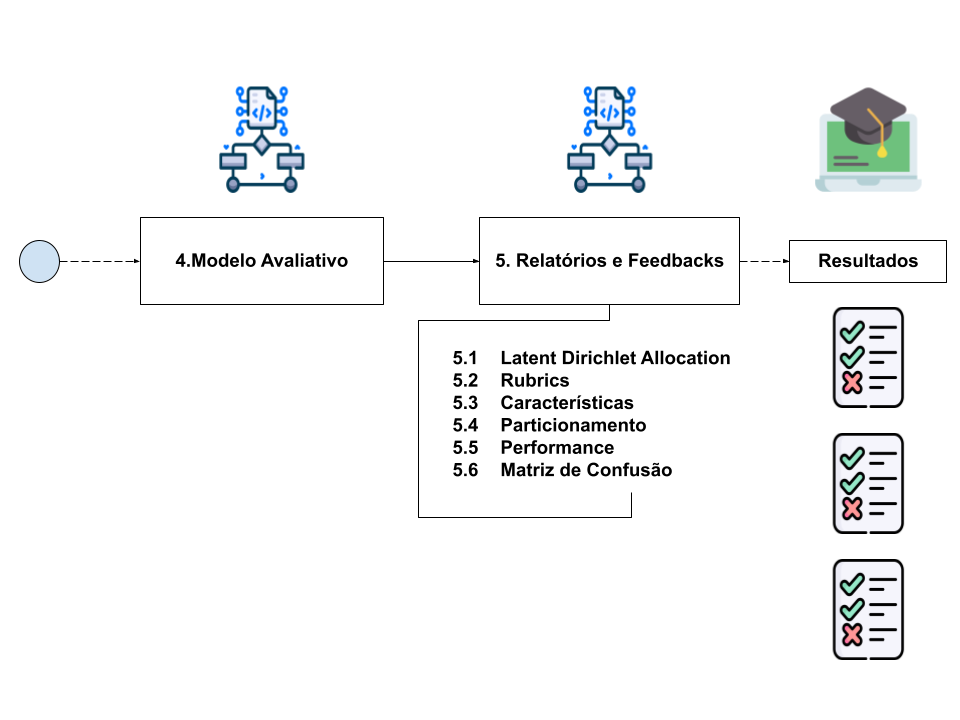
\includegraphics[width=\textwidth]{figuras/esquema-rf-pNota.png}
\caption{Módulo de \textit{Relatórios e Feedbacks} no esquema do \textit{p}Nota.}
\label{fig-rf}
\end{figure}


Conforme a etapa apresentada na Figura \ref{fig-rf}, os relatórios precedem o envio dos resultados para o AVA, de forma a descrever o \textit{Modelo Avaliativo}. Com fundamento na relação entre termos e notas, a caracterização das respostas é determinante para conectar usuários com os métodos aplicados pelo \textit{p}Nota. Assim, os relatórios e os \textit{feedbacks} devem descrever em detalhes a forma de avaliação aplicada para instruir os usuários. Um exemplo completo dos relatórios é apresentado no Apêndice \ref{exemplo-pNota}.

Os procedimentos de descrição do \textit{p}Nota incluem, desde características superficiais, conectadas às calibrações e às etapas do sistema, até características mais profundas, que contextualizam a interpretação do sistema sobre a atividade. É possível citar como exemplos do primeiro os \textit{clusters} formados, amostras selecionadas para anotação ou características mais frequentes. No segundo, por outro lado, são apresentados em linguagem natural os resultados e a proximidade entre as notas.


\subsection{Relatório dos Processos}
\label{subsec-relatorio-processos}

Os relatórios buscam passar por cada etapa do \textit{p}Nota para mostrar como foram as interações com o professor e os resultados obtidos. Um desses é o relatório de esforço de anotação e treinamento do algoritmo. Retomando o exemplo do Capítulo \ref{cap1-intro}, na Tabela \ref{tab-ptasag-train-46} é apresentado tal relatório para a atividade 46 do \textit{dataset PTASAG}.

\begin{table}[!b]
\centering
\caption{Particionamento das amostras em treino e teste na atividade exemplo \textit{PTASAG Atividade 46}.}
\label{tab-ptasag-train-46}
\begin{tabular}{|c c c c|} \hline
\multicolumn{3}{|l}{Dataset} & Amostras\\ 

\multicolumn{3}{|l}{PTASAG : Atividade 46} & 655 \\ \hline 

Treino (Un.) & Treino (\%)  & Teste (Un.) & Teste (\%) \\ \hline 

524 & 80.0 & 131 & 20.0 \\ 

\hline \hline
\end{tabular}
\end{table}


Na Tabela \ref{tab-ptasag-train-46} é apresentado um exemplo de relatório utilizado para explicar o que foi realizado em um dos processos. O mesmo informa qual foi o particionamento de amostras utilizado e qual foi o esforço de correção do professor. Porém, o nível descritivo deve ser maior quando caracterizamos aspectos avaliativos, tornando cada vez mais transparente a avaliação. Durante a elaboração destes, identifica-se uma certa dificuldade de interpretação das métricas categóricas em relação ao observado com métricas contínuas. Por conta disso, são estabelecidos três níveis de desempenho para as métricas percentuais: \textit{Avançado}, \textit{Adequado} e \textit{Insuficiente} \cite{nascimento2020}.

\begin{itemize}
	\item Intervalo de 75\% - 100\%: Nível \textcolor{green}{Avançado};
	\item Intervalo de 35\% - 75\%: Nível \textcolor{yellow}{Adequado};
	\item Intervalo de 0\% - 35\%: Nível \textcolor{red}{Insuficiente}.
\end{itemize}


Os níveis são similares aos que o professor utiliza para determinar o conteúdo assimilado pelos alunos durante a avaliação \cite{nascimento2020}. Em nível \textcolor{red}{Insuficiente} a relação entre as notas finais divulgadas pelo professor e as notas do sistema apresenta índices abaixo do esperado. Em nível \textcolor{yellow}{Adequado} as notas apresentam alinhamento com as que foram atribuídas pelo professor. E em nível \textcolor{green}{Avançado}, os resultados do modelo avaliativo foram próximos aos divulgados pelo especialista, identificando bem seu método avaliativo. Assim, foi necessário trazer para a realidade em sala de aula os resultados da classificação, tal qual já é a realidade quando é aplicado o nível de erro entre avaliadores \cite{almeida-junior2017}. Na Figura \ref{fig-ptasag-performance-46} é apresentado o desempenho de categorização conforme esses três níveis.

\begin{figure}[!t]
 \centering
 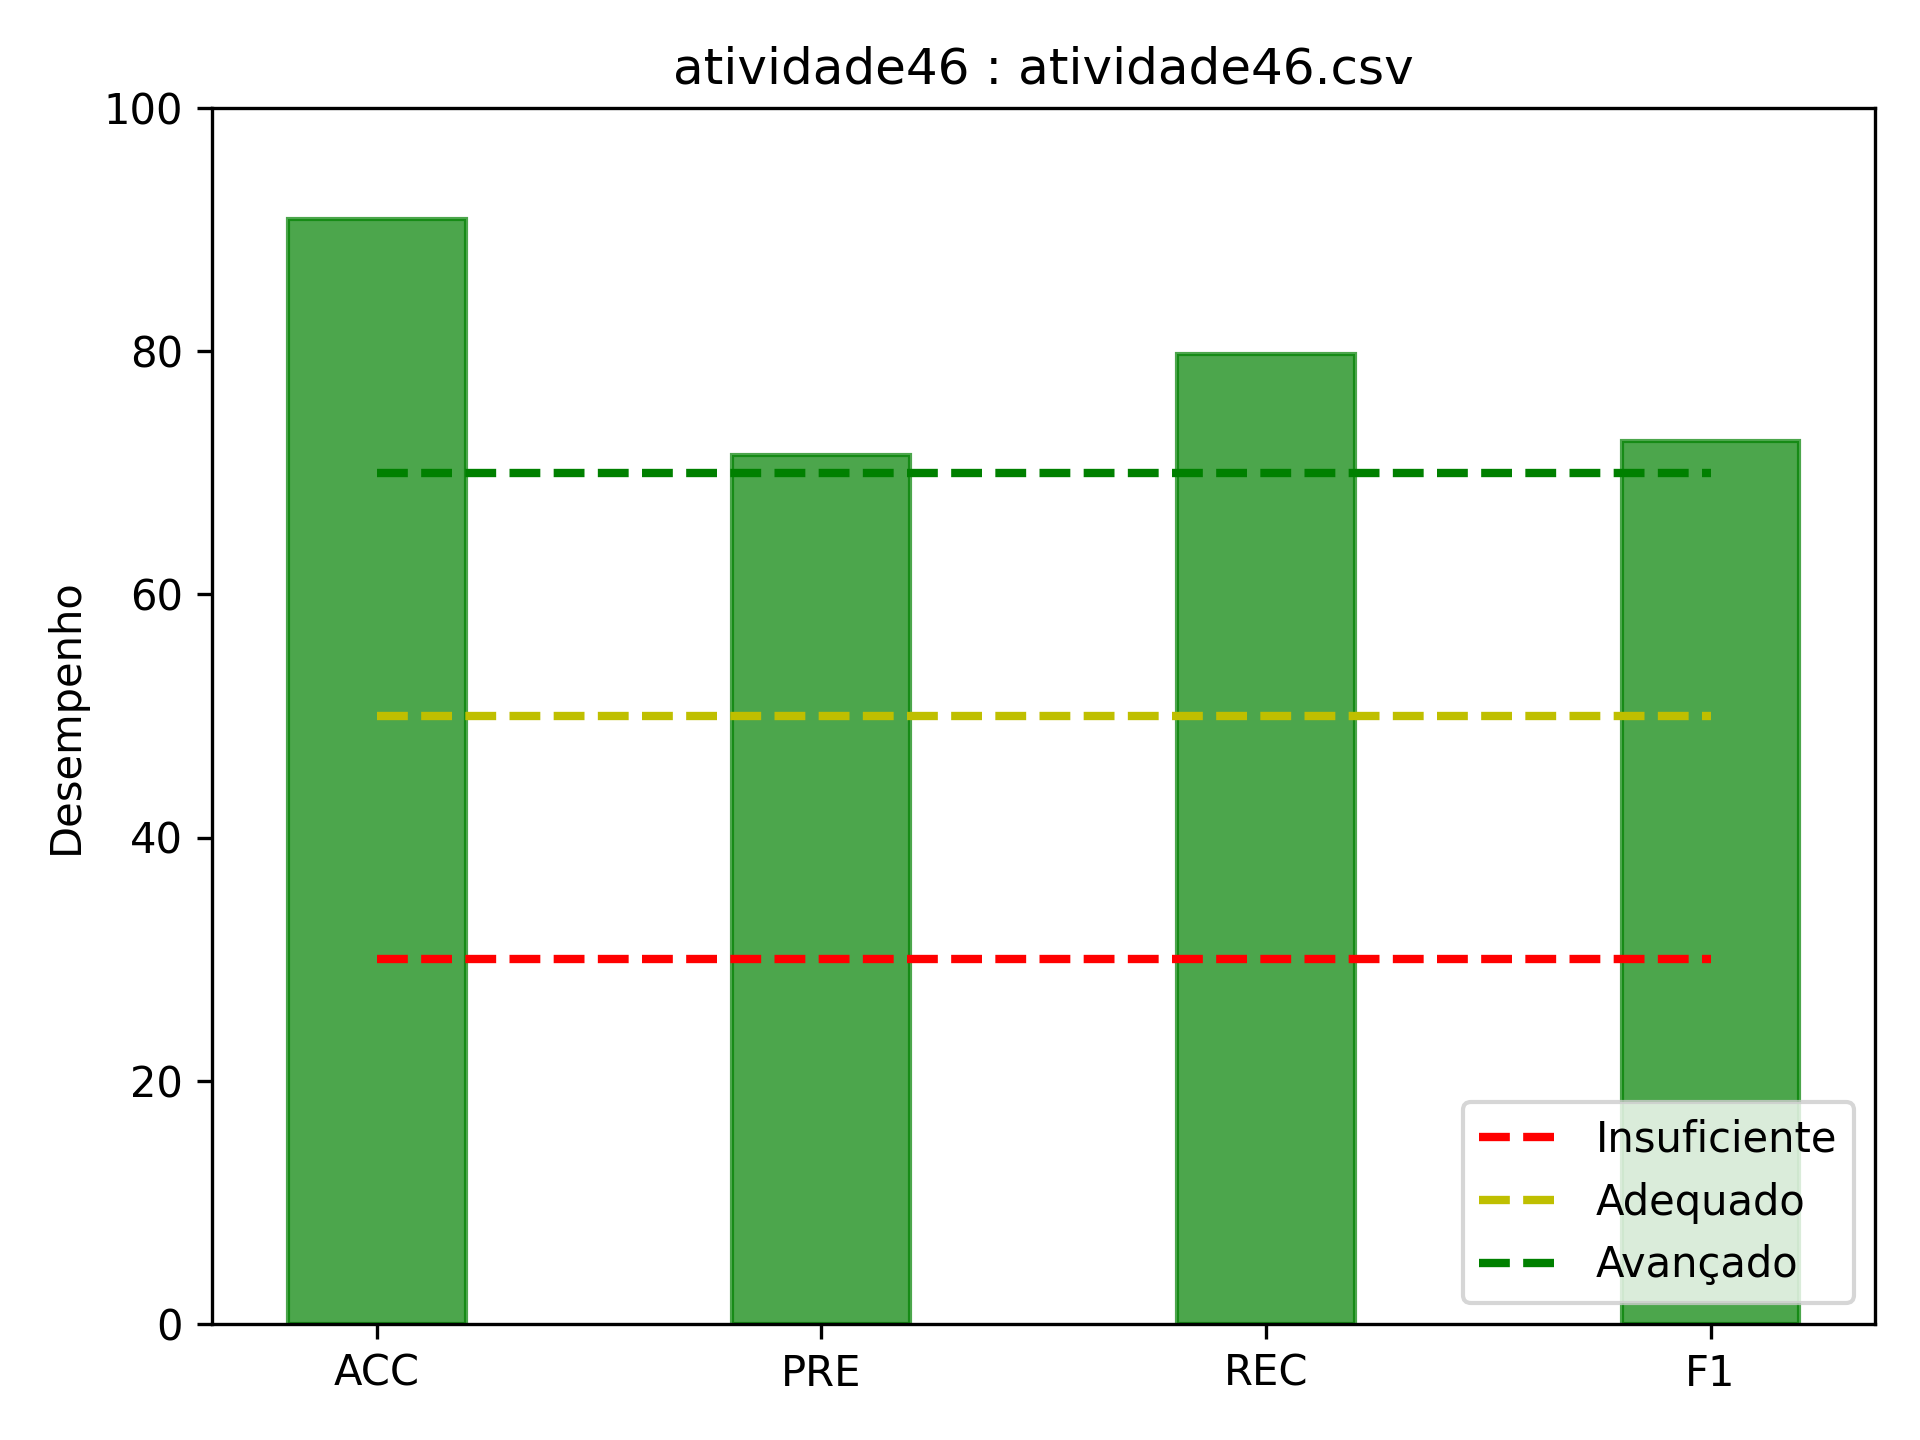
\includegraphics[width=0.8\textwidth]{figuras/exemplo/exemplo-ptasag-rdf.png}
 \caption{Resultados de desempenho do exemplo \textit{PTASAG Atividade 46}.}
 \label{fig-ptasag-performance-46}
\end{figure}

Na Figura \ref{fig-ptasag-performance-46}, há um resultado de alto desempenho de classificação usando o classificador RDF. Com os níveis e as cores, os resultados e as métricas de avaliação tornam-se um pouco mais simples para interpretação e análise dos professores, sendo assim, uma ferramenta útil para comparação e uso na sua rotina de validação do sistema.


\subsection{\textit{Feedbacks} Contextuais}
\label{subsec-feedbacks-contextuais}

Os \textit{feedbacks} contextuais são métodos que descrevem como foi o comportamento da avaliação segundo o conteúdo. Esses métodos aplicam-se diretamente à realidade da disciplina e visam caracterizar o vínculo textual de cada nível de nota. O objetivo é levar para as salas de aula um material que apoia os estudantes na compreensão da disciplina, dando suporte ao método do professor.

O primeiro modelo realiza a aplicação de cores nas respostas, identificando quais são as palavras mais correlacionadas com cada nota. Essa técnica é realizada com otimização por Algoritmo Genético \cite{spalenza2016a} ou com Lime\footnote{Lime - https://github.com/marcotcr/lime}. O Lime é uma ferramenta de visualização que descreve o processo de classificação de acordo com os padrões do conteúdo \cite{ribeiro2016}. Em ambos, a ideia é atribuir coloração por nota e mostrar os termos mais correlacionados com cada uma das classes. Assim, associa-se a menção de cada termo com a nota recebida pela resposta e seu alinhamento, definindo \textit{status} negativo ou positivo. Na Figura \ref{fig-highlight-46}, identificam-se termos que ampliam a relação da resposta com a nota 3 atribuída.

\begin{figure}[!h]
 \centering
 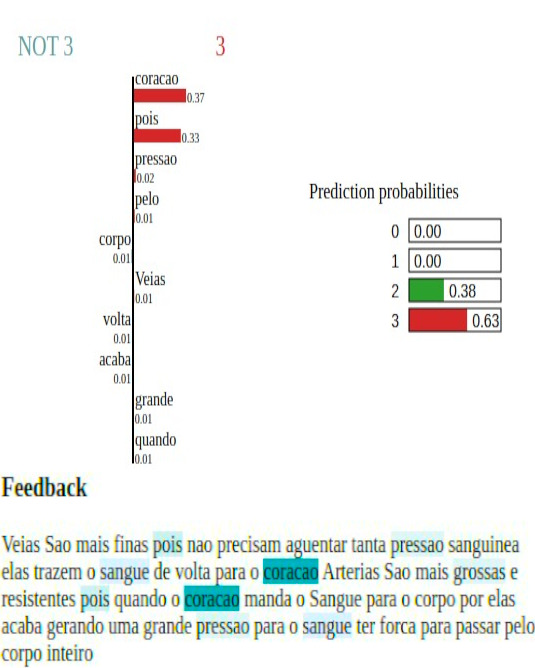
\includegraphics[width=.75\textwidth]{figuras/exemplo/highlight.jpeg}
 \caption{Destaques nos principais termos da resposta do estudante \#1995 do \textit{PTASAG Atividade 46}.}
 \label{fig-highlight-46}
\end{figure}

Como é exposto na Figura \ref{fig-highlight-46}, os termos \textit{coração}, \textit{sangue} e \textit{pressão} são destaques dessa resposta. Porém, os termos poderiam ser encontrados nas demais respostas. Por isso, foi identificado que o contexto apresenta 63\% de correlação com demais menções que receberam nota 3. Um segundo modelo, também em níveis textuais, extrai o conteúdo chave, de acordo com os tópicos mencionados por nível de nota. Nesse nível aplica-se LDA \cite{hoffman2013} no reconhecimento da composição de nota, ou seja os termos que em tese são essenciais para receber cada uma das classes. O LDA é uma técnica que aplica estatística descritiva para equivalência parcial dos dados. Nesse caso, a identificação da compatibilidade vetorial entre os textos que compõem um determinado nível de nota \cite{sahu2020}. Portanto, os dois são complementares. Enquanto o primeiro observa cada resposta pela perspectiva da avaliação, o segundo realiza o oposto. 

Apesar do acompanhamento da dinâmica do sistema no processo avaliativo, é complexo ao sistema identificar padrões coerentes de resposta. Para isso, utiliza-se o quadro de \textit{rubrics} para representar o modelo avaliativo elaborado pelo sistema em conjunto com o professor. O quadro de \textit{rubrics} é um modelo de caracterização do processo avaliativo conforme o modelo de resposta esperado para cada nota. Após o processo avaliativo, este torna-se um descritor, determinando na perspectiva dos estudantes quais foram as principais características elencadas para cada nota. Na Tabela \ref{tab-rubrics-exemplo} há um exemplo do quadro de \textit{rubrics} para a nota 3 da \textit{Atividade 46}.

\begin{table}[!h]
\centering
\caption{Tabela de \textit{rubrics} para as duas notas encontradas na atividade exemplo e as respostas mais alinhadas com as palavras selecionadas pelo LDA.}
\label{tab-rubrics-exemplo}
\footnotesize
\begin{tabular}{ p{2cm} | p{14cm}}
\multicolumn{2}{l}{\textbf{PTASAG : Atividade 46}} \\ \hline
\multicolumn{2}{c}{\textbf{Nota: 3}} \\ \hline 
\multicolumn{2}{l}{\textit{T{\'o}picos: arterias coracao corpo levam pressao rico sangue veias}} \\ \hline
 \# & Exemplos \\ \hline
19 & Veias \textit{levam} o \textit{sangue} para o \textit{coracao} e as \textit{arterias} \textit{levam} o \textit{sangue} do \textit{coracao} As \textit{veias} sao mais finas e as \textit{arterias} sao grossas e resistentes\\ \hline
78 & As \textit{veias} \textit{levam} \textit{sangue} ate o \textit{coracao} elas nao aguentam muita \textit{pressao} As \textit{arterias} \textit{levam} o \textit{sangue} do \textit{coracao} para o resto do \textit{corpo} pois aguentam maior \textit{pressao} e sao maiores\\ \hline
242 & As \textit{veias} \textit{levam} \textit{sangue} do \textit{corpo} para o \textit{coracao} onde ele possa ser bombeado novamente para o \textit{corpo} As \textit{arterias} saem do \textit{coracao} tornando se cada vez mais finas esses vasos \textit{levam} o \textit{sangue} nutrientes e oxigenio do \textit{coracao} para os tecidos\\ \hline
328 & As \textit{arterias} transportam o \textit{sangue} que sai do \textit{coracao} inicialmente \textit{rico} em O2 as diversas partes do \textit{corpo} as \textit{veias} recolhem esse \textit{sangue} \textit{rico} em CO2 e \textit{levam} de volta para o \textit{coracao} As \textit{arterias} possuem paredes mais grossas e as \textit{veias} possuem valvulas que impedem o \textit{sangue} de voltar\\ \hline
372 & As \textit{veias} \textit{levam} \textit{sangue} do \textit{corpo} ao \textit{coracao} e as \textit{arterias} do \textit{coracao} ao \textit{corpo} Alem disso as \textit{arterias} sao mais grossas que as \textit{veias} para suportar \textit{pressao}\\ \hline
444 & As \textit{veias} realizam o transporte do \textit{sangue} venoso \textit{rico} em CO2 no sentido do \textit{corpo} para o \textit{coracao} Ja as \textit{arterias} carregam o \textit{sangue} \textit{rico} em O2 do \textit{coracao} para o \textit{corpo} Alem disso as \textit{arterias} sao mais grossas que as \textit{veias} pois tem que aguentar a \textit{pressao} exercido pelos batimentos cardiacos que bombam o \textit{sangue}\\ \hline
456 & As \textit{arterias} sao vasos sanguineos responsaveis por conduzir o \textit{sangue} para fora do \textit{coracao} carregando \textit{sangue} artereal \textit{rico} em O2 As \textit{veias} sao responsaveis por conduzir o \textit{sangue} proveniente dos tecidos para o \textit{coracao} onde e \textit{rico} em CO2 e carrega \textit{sangue} venoso\\ \hline
479 & As \textit{veias} \textit{levam} o \textit{sangue} dos tecidos para o \textit{coracao} e possuem baixa \textit{pressao} ja as \textit{arterias} possuem alta \textit{pressao} e \textit{levam} \textit{sangue} do \textit{coracao} para o \textit{corpo}\\ \hline
\hline
\end{tabular}
\end{table}

Na Tabela \ref{tab-rubrics-exemplo} foram coletados os tópicos mais relevantes em cada uma das categorias para destacar os principais termos das respostas. No exemplo a resposta nota 3 fica evidente. Esta deve citar a relação entre o \textit{corpo} e o \textit{coração}, com a \textit{pressão} \textit{arterial} levando o sangue, e retornando pelas \textit{veias}. Então, a função do \textit{rubrics} é definir os padrões de resposta do sistema e, adicionalmente, criar relatórios que expliquem o formato avaliativo em apoio ao professor.

% ==============================================================================
% TCC - Nome do Aluno
% Capítulo 3 - Avaliação do Trabalho
% ==============================================================================
\chapter{Experimentos e Resultados}
\label{cap-experimentos}

O \textit{p}Nota é um sistema que foi produzido com o andamento de experimentos em plataformas AVA na Universidade Federal do Espírito Santo (UFES). Nesse período, durante o desenvolvimento adicionamos diferentes técnicas para desenvolver a compreensão linguística e avaliativa do modelo SAG proposto. Os testes envolveram um conjunto de atividades com mais de 126 questões e 2805 respostas \cite{spalenza2016a}. Nestes testes foram analisadas formas distintas de escrita e em diferentes níveis de instrução, do Ensino Básico à Pós-Graduação, abordando tópicos distintos como Computação, Arquivologia, Ciências, Filosofia, Economia e Medicina. Entretanto, para avaliar o sistema apresentamos aqui uma série de experimentos com \textit{datasets} encontrados na literatura.

Esse capítulo apresenta os experimentos das duas etapas avaliativas. A primeira avalia a parte fundamental da técnica de \textit{Active Learning} do sistema \textit{p}Nota, com o uso da \textit{clusterização} para a identificação dos principais itens de resposta em cada base de dados. Na sequência, a segunda apresenta os métodos de classificação, a qualidade do aprendizado do sistema na predição de notas e sua adequação ao modelo esperado pelo tutor.

\section{\textit{Datasets}}

De acordo com a literatura, selecionamos nove bases de dados, em português e inglês. Cada base de dados foi utilizada conforme a sua disponibilidade e suas características. Alguns \textit{datasets} estão em linguagens que seria possível o processamento mas precisamos de maior conhecimento da linguagem para adaptação do \textit{p}Nota, como o \textit{JapaneseSAS} (japonês) \cite{ishioka2017}, \textit{Cairo University Dataset} (árabe) \cite{gomaa2019}, \textit{Corpus of Reading comprehension Exercises in German (CREG)} (alemão) \cite{ziai2012}, \textit{Science Answer Assessment (ScAA)} (hindi) \cite{agarwal2020} e o \textit{Chinese Educational Short Answers (CESA)} (chinês) \cite{ding2020}. Outros \textit{datasets} foram descartados pela indisponibilidade, como o \textit{Critical Reasoning for College Readiness (CR4CR) Assessment} \cite{condor2021}, o \textit{Cordillera Corpus} \cite{zhang2020}, dentre outros inúmeros privados. Nesse caso se enquadram grande quantidade de artigos, com coleta de dados local e sem acesso público. Dentre as nove citadas na literatura que tivemos acesso, organizamos por formato das notas atribuídas: ordinais, discretas e contínua \cite{morettin2010}. 

Em bases de dados com notas \textit{ordinais} o método avaliativo do tutor é dado de forma textual e categórica. A representação do rótulo não estabelece escalas para o sistema, não sendo possível mensurar a diferenças na escala \textit{a priori}. O modelo formado deve compreender as estruturas textuais de forma simbólica, caracterizando a essência de cada nível. Portanto, o classificador deve ser robusto para aprender a relevância das respostas pela equivalência de palavras-chave. Basicamente, é fundamental para o classificador produzir um modelo com as informações essenciais para a resposta receber tal categoria e reproduzir o modelo.

Por outro lado, outra situação acontece com bases de dados avaliados com notas contínuas. As notas \textit{contínuas} não apresentam níveis, mas sim intervalos numéricos. As respostas recebem notas de acordo com o intervalo avaliativo. Apesar de numérico, o fato da variável não definir uma categoria que represente a divergência entre respostas dificulta o aprendizado do modelo avaliativo. Ao sistema, isso torna subjetiva a espectativa de resposta subjetivo. Assim, esse tipo de atividade é avaliada por interpolação. Nesse caso, o sistema realiza uma regressão de acordo com os pontos conhecidos, gerando a nota pela referência ao grau de similaridade para as demais respostas.

Por fim, a avaliação \textit{discreta} numérica é a mais comum. Esse modelo favorece também os sistemas computacionais na criação da representação de resposta por categoria de nota. Ao tempo que a categoria induz a equivalência de todas as respostas ao qual foi associada. Assim, o sistema consegue mensurar equivalência e divergências pelos indícios de proximidade entre respostas avaliadas já conhecidas para além da mesma categoria. O desafio do sistema com este tipo de nota é criar um bom modelo de classificação que aprenda essa relação dupla. Para além da categoria das respostas, o sistema passa a ter que interpretar as informações fundamentais de cada classe e a escala de divergência para as demais categorias. A Tabela \ref{tab-datasets} apresenta os detalhes de cada \textit{dataset}, incluindo o número de questões, o total de respostas, o modelo avaliativo aplicado e a linguagem.

\begin{center}
\begin{table}[!h]
\begin{tabular}{r |c c c c} 
 \hline
 Dataset & Quest{\~o}es & Respostas & Modelo Avaliativo & Linguagem \\ \hline
 SEMEVAL2013 Beetle & 47 & 4380 & ordinal & Ingl{\^e}s \\
 SEMEVAL2013 SciEntsBank & 143 & 5509 & ordinal & Ingl{\^e}s \\
 Kaggle ASAP-SAS & 10 & 17043 & discreto & Ingl{\^e}s \\
 Powergrading & 10 & 6980 & discreto & Ingl{\^e}s \\
 UK Open University & 20 & 23790 & discreto & Ingl{\^e}s \\
 University of North Texas & 87 & 2610 & cont{\'i}nuo & Ingl{\^e}s \\
 Kaggle PTASAG & 15 & 7473 & discreto & Portugu{\^e}s \\
 Projeto Feira Liter{\'a}ria & 10 & 700 & discreto & Portugu{\^e}s \\
 VestUFES & 5 & 460 & cont{\'i}nuo & Portugu{\^e}s \\
 \hline
 \hline
\end{tabular}
\caption{Bases de dados e suas principais caracter{\'i}sticas.}
\label{tab-datasets}
\end{table}
\end{center}

A Tabela \ref{tab-datasets} descreve os nove \textit{datasets} utilizados nos experimentos deste capítulo. Através das características apresentadas, identificamos uma regularidade interna de cada \textit{dataset}. Entretanto, entre os \textit{datasets} existe uma variação muito grande com questões de 30 até mais de 1800 respostas. É importante destacar ainda que, a definição de respostas curtas e as características textuais das respostas de cada um destes \textit{datasets} foram apresentadas no Capítulo \label{cap1-intro}, em especial na Tabela \ref{tab-features}. No total, esse \textit{corpora} apresenta um total de 347 questões e 68.945 respostas. Cada base de dados e sua descrição completa é apresentada a seguir:


\subsection{Dataset \textit{Beetle} do \textit{SEMEVAL'2013 : Task 7} \textit{(Inglês)}}
\label{beetle-db}

\textit{Beetle} \cite{dzikovska2012} é um dos \textit{datasets} utilizados durante o \textit{International Workshop on Semantic Evaluation - SEMEVAL'2013}. O \textit{SEMEVAL} seleciona anualmente uma série de desafios em análise semântica e apresenta no formato de competição. O \textit{corpus Beetle} foi selecionado para a \textit{Task 7: The Joint Student Response Analysis and 8th Recognizing Textual Entailment Challenge} \cite{dzikovska2013}. Portanto, a competição consistia em duas propostas. A primeira é a análise e avaliação das respostas obtidas e a segunda o reconhecimento da relação textual entre as respostas coletadas e a expectativa de resposta do professor.

Esse \textit{dataset} consiste em uma coleção de interações entre estudantes e o sistema \textit{Beetle II}. Beetle II é um Sistema Tutor Inteligente (STI) para aprendizado de conhecimentos básicos em Eletricidade e Eletrônica do Ensino Médio. Os alunos foram acompanhados durante 3 a 5 horas para preparar materiais, construir e observar circuitos no simulador e interagir com o STI. Esse sistema faz questões aos alunos, avalia as respostas e envia \textit{feedbacks} via \textit{chat}. Na construção deste \textit{dataset} foram acompanhados 73 estudantes voluntários da \textit{Southeastern University} dos Estados Unidos.

Foram aplicadas questões categorizadas em dois tipos factuais e explicativas. As questões factuais requerem que o aluno nomeie diretamente determinados objetos ou propriedades. Equanto isso, as questões explicativas demandam que o aluno desenvolva a resposta em uma ou duas frases. Para a formação do \textit{dataset} foram adicionadas apenas as atividades do segundo tipo, pois representam maior complexidade para sistemas computacionais. No total foram selecionadas 47 questões com 4380 respostas. A avaliação foi feita conforme o domínio demonstrado sobre o assunto em cinco categorias: \textit{correct}, \textit{partially-correct-incomplete}, \textit{contradictory}, \textit{irrelevant} e \textit{non-domain}. Durante a anotação o coeficiente \textit{Kappa} obtido foi de 69\% de concordância.


\subsection{Dataset \textit{SciEntsBank} do \textit{SEMEVAL'2013 : Task 7} \textit{(Inglês)}}
\label{scientsbank-db}

O \textit{corpus Science Entailments Bank (SciEntsBank)} \cite{dzikovska2012} é um dos \textit{datasets} utilizados durante o \textit{International Workshop on Semantic Evaluation - SEMEVAL'2013} \cite{dzikovska2013}, com foco na avaliação de sistemas conforme a sua capacidade de análise e exploração semântica da linguagem. É uma base de dados formadas pela avaliação de questões da disciplina de Ciências. Na avaliação 16 assuntos distintos são abordados entre ciências físicas, ciências da terra, ciências da vida, ciências do espaço, pensamento científico e tecnologia. 

As questões são parte da \textit{Berkeley Lawrence Hall of Science Assessing Science Knowledge (ASK)} com avaliações padronizadas de acordo com o material de apoio \textit{Full Option Science System (FOSS)}. Participaram estudantes dos Estados Unidos de terceira a sexta série, coletando em torno de 16 mil respostas. Porém, dentre as questões de preenchimento, objetivas e discursivas, foram utilizadas apenas as discursivas, que requisitavam explicações dos alunos segundo o tema. As respostas foram graaduadas em cinco notas ordinais: \textit{correct}, \textit{partially-correct-incomplete}, \textit{contradictory}, \textit{irrelevant} e \textit{non-domain}. Portanto, o \textit{SciEntsBank} consiste em um conjunto com 143 questões selecionadas e 5509 respostas. No processo de avaliação foi observado o coeficiente \textit{Kappa} com 72.8\% de concordância.

\begin{comment}
[('contradictory', 557), ('correct', 2241), ('irrelevant', 1248), ('non_domain', 26), ('partially_correct_incomplete', 1437)] 5509 SCIENTSBANK

[('contradictory', 1160), ('correct', 1841), ('irrelevant', 130), ('non_domain', 218), ('partially_correct_incomplete', 1031)] 4380 BEETLE 
\end{comment}

\subsection{Dataset do Concurso ASAP-SAS no \textit{Kaggle} \textit{(Inglês)}}
\label{kaggle-db}

A origem da base de dados \textit{ASAP - SAS}, \textit{Automated Student Assessment Prize - Short Answer Scoring} é uma competição proposta pela \textit{Hewllet Foundation} na plataforma \textit{Kaggle} \footnote{The Hewlett Foundation - Short Answer Scoring: https://www.kaggle.com/c/asap-sas}. A competição consistiu em três fases:

\begin{itemize}
\item Fase 1:  Demonstração em respostas longas (redações); 
\item Fase 2:  Demonstração em respostas curtas (discursivas);
\item Fase 3:  Demonstração simbólica matemática/lógica (gráficos e diagramas).
\end{itemize}

Seu objetivo era descobrir novos sistemas de apoio ao desenvolvimento de escolas e professores. Especificamente, as três fases destacam a atividade lenta e de alto custo de avaliar manualmente testes, mesmo que com padrões bem definidos. Uma consequência disso é a redução do uso de questões discursivas nas escolas, dando preferência para as questões objetivas para evitar a sobrecarga de trabalho. Isso evidencia uma gradativa redução da capacidade dos professores em incentivar o pensamento crítico e as habilidades de escrita. Portanto, os sistemas de apoio, são uma possível solução para suportar os métodos de correção, avaliação e feedback ao conteúdo textual dos alunos.

Neste contexto, a competição apresentou 10 questões multidiciplinares, de ciências à artes. Estão distribuidas 17043 respostas de alunos dentre essas atividades. Para chegar nessa quantidade, foram selecionadas por volta de 1700 respostas dentre 3000 respostas em cada atividade. Cada resposta tem aproximadamente 50 palavras. A primeira avaliação foi dada pelo primeiro especialista como nota final e a segunda nota foi atribuída apenas para demonstrar o nível de confiança da primeira nota. A avaliação apresentada por dois especialistas apresentou concordância de 90\% no coeficiente \textit{Kappa}.


\subsection{Dataset \textit{Powergrading} \textit{(Inglês)}}
\label{powergrading-db}
Elaborado através do \textit{United States Citizenship Exam} (USCIS) em 2012, a base de dados \textit{Powergrading} contém 10 questões e 6980 respostas \cite{basu2013}. Desenvolvida originalmente para destacar a possibilidade de avaliação massiva, o \textit{dataset} selecionou 698 respostas para cada uma das questões. As respostas foram geradas com \textit{Amazon Mechanical Turk}, serviço remoto de análise manual de conteúdo para anotação da \textit{Amazon}. Foi coletada por um grupo de pesquisa da \textit{Microsoft}\footnote{Powergrading: https://www.microsoft.com/en-us/download/details.aspx?id=52397} e cada questão acompanha um modelo de resposta e as respostas recebidas para cada questão.  Além disso, acompanha o \textit{dataset} outras 10 questões não avaliadas.

Foram requisitadas respostas com poucas palavras, atingindo no máximo uma ou duas sentenças. Por conta disso, os resultados são respostas muito curtas com 4 palavras em média. Em geral, por conta da convergência, vários padrões de resposta se repetem \cite{riordan2017}. Com avaliações binárias, 1 para resposta correta e 0 para incorreta, cada resposta apresenta avaliações de três diferentes tutores. Apesar de alguns trabalhos assumirem um dos avaliadores como padrão, utilizamos como modelo de avaliação a resultante da comparação entre os três. Apesar de não ter complexidade linguística, ocorreu contradição entre os avaliadores em 470 respostas. Em valores percentuais, isso representa 7\% do total de respostas do conjunto de dados.

\begin{comment}
Respostas não coincidentes em cada questão
q1 - 1 q2 - 12 q3 - 145 q4 - 45 q5 - 18 q6 - 52 q7 - 20 q8 - 17 q13 - 108 q20 - 52
\end{comment}

\subsection{Dataset da \textit{UK Open University} \textit{(Inglês)}}
\label{openunv-db}

A base de dados da \textit{UK Open University} é um conjunto de questões coletadas na disciplina de introdução à ciências, denominada \textit{S103 - Discovering Science} \cite{jordan2012}. O foco do conjunto de atividades são abordagens em questões factuais bem concisas, não excedendo 20 palavras. Os alunos receberam as atividades através do ambiente da \textit{Intelligent Assessment Technologies (IAT)}, o \textit{FreeText Author}. O \textit{FreeText Author} foi utilizado como um método de \textit{CAA} de modo interativo e com resultado automático analizando a resposta do aluno segundo os padrões de resposta conhecidos. O sistema permitiu uma sequência de envios e apresentava comentários da resposta como \textit{feedback} para os alunos. Dependendo da complexidade da resposta, o tempo de retorno dos resultado varia muito entre alguns poucos minutos até mais do que um dia.

O \textit{dataset} é de acesso privado, mas foi disponibilizado pelos autores para este estudo. Dentre suas 20 questões, esse \textit{dataset} apresenta diferentes quantidades de respostas entre 511 e 1897. A avaliação é discreta e binária, definindo cada resposta como correta ou incorreta. Não existe notas intermediárias, representando diretamente se o aluno atendeu ou não os requisitos da resposta. 


\subsection{Dataset da \textit{University of North Texas} \textit{(Inglês)}}
\label{ntexasunv-db}

O \textit{dataset} da \textit{University of North Texas - UNT} \cite{mohler2011}, conhecido como \textit{Texas dataset} \footnote{Texas Dataset: https://web.eecs.umich.edu/{\textasciitilde}mihalcea/downloads.html}, é uma coleção de questões discursivas extraída no curso de Ciência da Computação. Composta por 80 atividades únicas, esse conjunto é composto por dez listas de exercícios com até sete questões e dois testes com dez questões cada. Foram aplicados em um ambiente virtual de aprendizagem durante a disciplina de Estrutura de Dados para 31 alunos. No total o \textit{dataset} é composto por 2273 respostas de alunos dentre as 80 atividades.

A avaliação foi feita com cinco notas discretas, de 5 equivalente a resposta perfeita até 0 completamente incorreta. Foram avaliadas por dois avaliadores independentes, estudantes do curso de Ciência da Computação. Para os autores, o modelo seguido pelo sistema deve ser a resultante da média ente os avaliadores, em intervalo contínuo. Dentre as notas atribuídas, 57,7\% das respostas receberam a mesma nota. Enquanto isso, um nível de diferença entre as notas representou 22,9\% do total de respostas. Foi constatado também que, dentre as diferenças na avaliação, o avaliador 1 atribuia maiores notas 76\% das vezes.

\subsection{Dataset \textit{PTASAG} no \textit{Kaggle} \textit{(Português)}}
\label{ptasag-db}

A \textit{PTASAG - Portuguese Automatic Short Answer Grading Data} é uma base de dados brasileira apresentada por \cite{galhardi2018b} e disponibilizada na plataforma \textit{Kaggle} \footnote{PT-ASAG-2018: https://www.kaggle.com/lucasbgalhardi/pt-asag-2018}. Foi coletada pela Universidade Federal do Pampa - Unipampa em conjunto com cinco professores de biologia do Ensino Fundamental. Foram criadas 15 atividades com base no sistema Auto-Avaliador CIR. Em biologia, os tópicos abordados foram sobre o corpo humano. Cada questão acompanha uma lista de conceitos, as respostas avaliadas e as respostas candidatas criadas pelos professores como referência. Foram criadas entre duas e quatro respostas candidatas contendo entre três e seis palavras-chave.

As atividades foram aplicadas ao Ensino Fundamental para 326 estudantes de 12 a 14 anos do 8\textsuperscript{\b{o}} e 9\textsuperscript{\b{o}} ano. Somados a estes, também foram aplicados a 333 alunos do Ensino Médio de 14 a 17 anos. As respostas foram avalidas por 14 estudantes de uma turma do último ano, considerando uma escala de notas de 0 a 3:

\begin{itemize}
\item Nota 0: Majoritariamente incorreta, fora de tópico ou sem sentido;
\item Nota 1: Incorreta ou incompleta mas com trechos corretos;
\item Nota 2: Correta mas com importantes trechos faltantes;
\item Nota 3: Majoritariamente correta apresentando os principais pontos.
\end{itemize}

No total, participaram 659 estudantes com um total de 7473 respostas. Cada uma das 15 questões apresenta entre 348 e 615 respostas. Apenas 4 questões foram avalidas por mais de um avaliador para verificar a concordância entre avaliadores. O coefficiente \textit{Kappa} observado foi de, em média, 53.25\%.


\subsection{Dataset do Projeto Feira Literária das Ciências Exatas \textit{(Português)}}
\label{findes-db}

É um conjunto de dados coletados durante o Projeto Feira Literária das Ciências Exatas \cite{nascimento2020}. As questões foram obtidas durante uma Atividade Experimental Problematizada por meio de um livro paradidático, ou seja, cujo objetivo primário não é o apoio didático. O livro escolhido foi \textit{A Formula Secreta} de David Shephard. 

Conforme o livro, os professores formularam 10 atividades e ministraram para 70 alunos do 5º ano de Ensino Fundamental. Essas atividades ministradas descreviam situações práticas de Química básica. No total, o conjunto de dados conta com 10 questões, 700 respostas e suas respectivas avaliações.


\subsection{Dataset do Vestibular UFES \textit{(Português)}}
\label{vest-ufes-db}

A base de dados VestUFES \cite{pissinati2014} é uma amostra das questões discursivas de Português do vestibular da UFES em 2012. A amostra selecionada contém 460 respostas divididas igualmente entre as 5 questões de língua portuguesa, também referentes a respostas dadas por 92 diferentes alunos.

Cada resposta foi avaliada por dois avaliadores. De acordo com o vestibular da universidade, os a avaliadores atribuíram notas entre 0 e 2 pontos em cada questão, totalizando 10 na soma da prova. Caso houvesse divergências de mais de 1 ponto entre as correções um terceiro avaliador era acionado para reavaliar a coerência das notas. A nota das respostas do \textit{dataset} foram redimensionadas pelo autor para o intervalo de 0 a 10 pontos. Na nova escala, as diferenças observadas entre os avaliadores foi de, em média, 1,38 pontos com desvio padrão de 1,75.


\begin{comment}
\subsection{Dataset das Disciplinas UFES \textit{(Português)} \label{disciplinas-ufes-db}
Essa base de dados foi coletada de algumas disciplinas ministradas na Universidade Federal do Espírito Santo - UFES entre 2015 e 2016 através do Moodle do Laboratório Computação de Alto Desempenho - LCAD. Entre as disciplinas estão Metodologia e Técnicas de Pesquisa Científica, Filosofia e Tecnologia da Informação II. Totalizando 45 atividades, neste \textit{dataset} foram recebidas 1162 submissões com média 25,82 e desvio padrão de 13,54 respostas por atividade.

O diferencial dessa base de dados é a mudança de características nas respostas encontradas nas múltiplas disciplinas, professores e alunos. Observam-se alterações consideráveis quanto ao tamanho, número de grupos, critério avaliativo ou objetividade. 
\end{comment}


\section{Experimentos}
\label{sec-experimentos}

Os experimentos realizados têm como intúito demonstrar a qualidade do método proposto de \textit{Active Learning}, com otimização do esforço de anotação humano. Assim, esperamos uma boa forma na amostragem tal qual o ganho de desempenho nos resultados de classificação. Através dos \textit{datasets} conhecidos da literatura, comparamos nossa proposta de análise das estruturas textuais em relação aos principais trabalhos publicados. Inicialmente os experimentos mostram o desempenho da etapa de \textit{clusterização} com a caracterização dos \textit{clusters} formados. Essa etapa indica a qualidade da amostragem em relação ao objetivo da atribuição de notas. Na sequência apresentamos comparativos com os classificadores da literatura, tentando maximizar os resultados obtidos com qualidade compatível aos demais trabalhos.


\subsection{Resultados de \textit{Clusterização}}
\label{sec-res-clustering}

Nessa primeira anális, observamos a qualidade dos \textit{clusters} formados. Assim, investigamos se a forma utilizada para construção dos \textit{clusters} foi efetiva para formação das amostras. Nessa etapa é essencial que a amostragem colete toda diversidade de notas, adquirindo conhecimento que torna possível comparar os níveis de nota. Neste identificamos as regiões que estabelecem diferenças entre contextos, com identificação de equivalências e divergências, isolando \textit{outliers}. Assim, essa primeira etapa é definitiva para a qualidade do aprendizado via \textit{Active Learning}.

A formação dos \textit{clusters} foi feita com base em uma otimização do \textit{elbow method}, caracterizando a dispersão das amostras \cite{spalenza2019}. Os resultados obtidos, visam ter \textit{clusters} mais homogêneos, segundo os índices de validação. O índice utilizado foio CVS, avaliando o coeficiente de variação do tamanho dos \textit{clusters} formados, evitando grande concentração. É um detalhe observado em \textit{clusters} com grandes percentuais de amostras os múltiplos contextos e a sobreposição entre as notas atribuídas. Na avaliação dos clusters, utilizamosas métricas CA, HS e CS, descritas na Seção \ref{subsec-clusterizacao}. Os resultados obtidos em cada um dos \textit{datasets} é apresentado na Tabela \ref{tab-clstr-index}.

\begin{table}[!h]
\centering
\caption{Bases de dados e índices qualitativos de \textit{clusterização}.}
\label{tab-clstr-index}
\begin{tabular}{r | r r r }
\hline
    \textit{Dataset}  & CA & HS & CS \\ \hline 
    SEMEVAL2013 Beetle & 0,5897 & 0,2895 & 0,1856 \\
    SEMEVAL2013 SciEntsBank SciEntsBank & 0,6064 & 0,2357 & 0,1789 \\
    UK Open University  & 0,7628 & 0,2825 & 0,0667 \\
    Projeto Feira Liter{\'a}ria & 0,6414 & 0,3920 & 0,2574 \\
    Kaggle ASAP-SAS  & 0,5364 & 0,1065 & 0,0741 \\
    Powergrading & 0,9032 & 0,6773 & 0,0760 \\
    Kaggle PTASAG  & 0,5208 & 0,2282 & 0,1418 \\
    University of North Texas & - & - & - \\
    VestUFES & - & - & - \\
\hline
\hline
\end{tabular}
\end{table}

Na Tabela \ref{tab-clstr-index} mostramos um alto índice de relação entre \textit{clusters} e itens que receberam uma mesma nota. Isso reflete em um CA médio de 65,15\%, atingindo até 90,32\% no \textit{dataset} \textit{Powergrading}. O CA, através do voto majoritário, indica quantas amostras compartilham \textit{clusters} com diferentes avaliações. Pela atribuição de notas contínuas, os \textit{datasets} \textit{University of North Texas} e \textit{VestUFES} foram desconsiderados nessa análise.

É um dos objetivos da etapa de clusterização que os grupos formados representem os tópicos abordados na questão. Assim, com efeito descritivo sobre os vínculos entre os \textit{cluster} e as notas, o CA indica o nível de complexidade para o reconhecimento de padrões e avaliação. No entanto, os índices HS e CS apontam a conexão entre cada classe de nota com os \textit{clusters} formados. Esses dois índices refletem algumas características dos problemas textuais.

O primeiro indica o nível de homogeneidade, ou seja, o percentual de \textit{clusters} formados por uma mesma nota. Estabelecer essa separabilidade entre classes e \textit{clusters} é uma tarefa muito complexa. Em especial na análise textual, são comuns as avaliações distintas ocorrerem em respostas com algum nível de sobreposição de termos. Ou seja, notas distintas podem apresentar algum nível de similaridade e formarem um mesmo \textit{cluster}. Já o segundo indica a equivalência entre os \textit{clusters} formados e cada uma das instância de nota. No entanto, dada a liberdade textual, dificilmente as respostas que recebem uma mesma nota apresentam os mesmos termos como referência.

Deste modo, \textit{datasets} com classificação binária tendem a ter alto desempenho na clusterização, como o \textit{Powergrading}. Porém, com muitos níveis de nota e textos maiores, \textit{datasets} como \textit{ASAP-SAS} e \textit{PTASAG}, tornam-se muito complexos para essa primeira etapa. O desempenho antes da etapa de amostragem mostra a eficiência dos classificadores para levar \textit{clusters} com divergências para uma melhoria considerável de desempenho. O desempenho das classificações após a amostragem é apresentada em detalhes na Seção \ref{sec-res-classificacao}. Para mostrar como os \textit{clusters} são formados por diferentes contextos, analisamos também a similaridade entre centróides. Indicando nesta etapa de \textit{Active Learning} que a \textit{clusterização} regionaliza as respostas segundo a interpretação dos contextos. A Figura \ref{fig-hmPowergrading} mostra qual foi o grau de similaridade encontrado nos \textit{clusters} formados para o \textit{dataset} \textit{Powergrading}.

\begin{figure}[!h]
\begin{minipage}[t]{.45\textwidth}
\centering
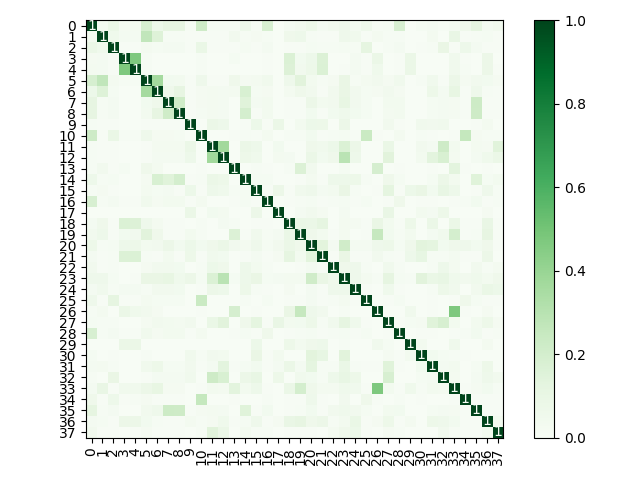
\includegraphics[width=\textwidth]{figuras/Powergrading/hm-q1.png} 
\subcaption{Atividade q1}
\end{minipage}%
\begin{minipage}[t]{.45\textwidth}
\centering
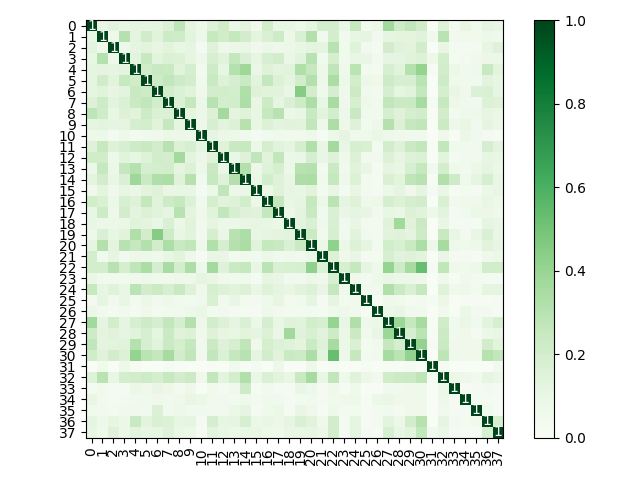
\includegraphics[width=\textwidth]{figuras/Powergrading/hm-q3.png} 
\subcaption{Atividade q3}
\end{minipage}%
\hfill
\begin{minipage}[t]{.45\textwidth}
\centering
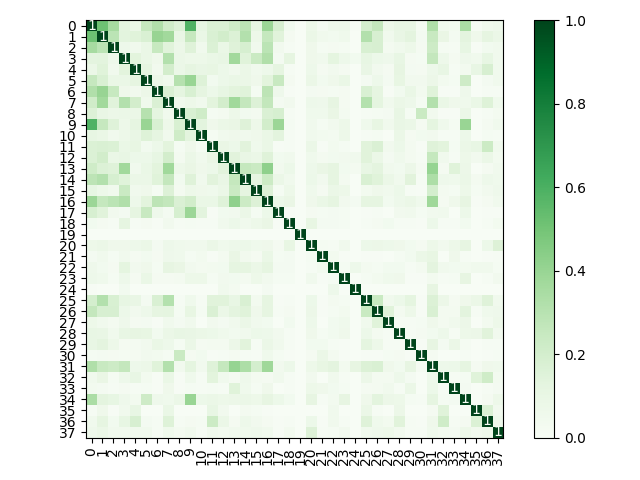
\includegraphics[width=\textwidth]{figuras/Powergrading/hm-q6.png} 
\subcaption{Atividade q6}
\end{minipage}%
\begin{minipage}[t]{.45\textwidth}
\centering
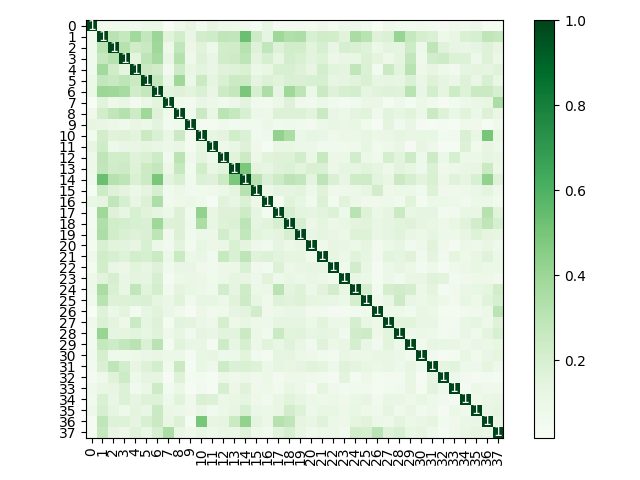
\includegraphics[width=\textwidth]{figuras/Powergrading/hm-q7.png} 
\subcaption{Atividade q7}
\end{minipage}
\caption{Similaridade entre \textit{centróides} para as atividades \textit{q1}, \textit{q3} e \textit{q6} e \textit{q7} em \textit{Powergrading}.}
\label{fig-hmPowergrading}
\end{figure}

Como observamos na Figura \ref{fig-hmPowergrading}, os grupos de respostas formados são muito consistentes, apresentando baixa similaridade para os demais \textit{clusters}. Há nesses casos uma divergência do item médio (\textit{centróide}) do \textit{cluster} em relação aos demais grupos.  Denominamos agrupamentos consistentes aqueles que todas as respostas têm um mesmo alinhamento, recebendo posteriormente uma mesma classe de nota. A atividade \textit{q1}, por exemplo, apresenta similaridade média de apenas 0,0355. Mesmo a que apresenta \textit{clusters} mais próximos, a atividade \textit{q7} apresenta em média 0,1387 de similaridade. As outras duas em destaque, atividades \textit{q3} e \textit{q6}, atingem 0,1207 e 0,0730. Assim, a clusterização têm potencial de formar zonas de equivalência e divergência com alta qualidade para as etapas de atribuição de notas. Essa alta qualidade indica \textit{clusters} bem separados de acordo com o contexto. A Figura \ref{fig-hmSciEntsBank} apresenta um caso oposto com a diferença entre os \textit{centróides} dos \textit{clusters} para a atividade \textit{SciEntsBank}.

\begin{figure}[!h]
\begin{minipage}[t]{.45\textwidth}
\centering
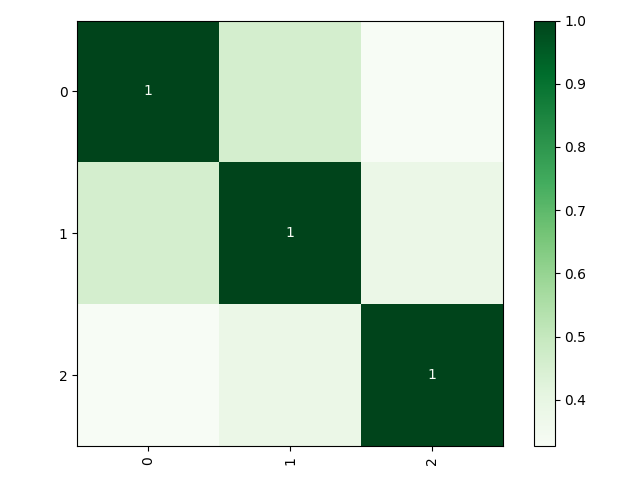
\includegraphics[width=\textwidth]{figuras/seb/hm-EM16b.png} 
\subcaption{Atividade EM16b}
\end{minipage}%
\begin{minipage}[t]{.45\textwidth}
\centering
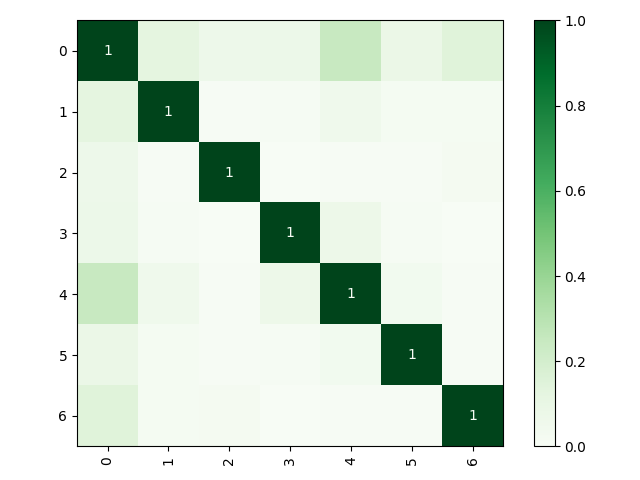
\includegraphics[width=\textwidth]{figuras/seb/hm-EM21b.png}
\subcaption{Atividade EM21b}
\end{minipage}%
\hfill
\begin{minipage}[t]{.45\textwidth}
\centering
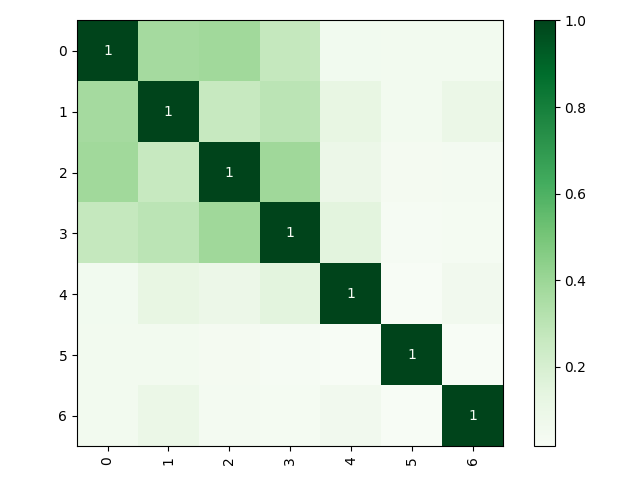
\includegraphics[width=\textwidth]{figuras/seb/hm-EM27b.png} 
\subcaption{Atividade EM27b}
\end{minipage}%
\begin{minipage}[t]{.45\textwidth}
\centering
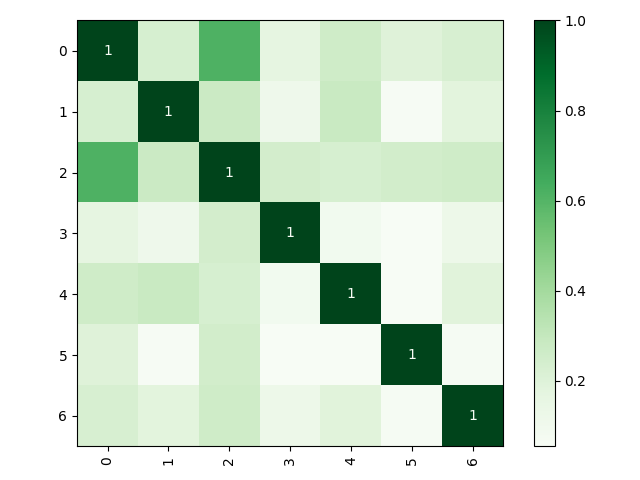
\includegraphics[width=\textwidth]{figuras/seb/hm-MX16a.png} 
\subcaption{Atividade MX16a}
\end{minipage}
\caption{Similaridade entre \textit{centróides} para as atividades \textit{EM16b}, \textit{EM21b}, \textit{EM27b} e \textit{MX16a} em \textit{SciEntsBank}.}
\label{fig-hmSciEntsBank}
\end{figure}

Como ilustrado na Figura \ref{fig-hmSciEntsBank}, temos clusterização mais complexa, em especial com poucas amostras. Diferente do que foi notado na questão anterior, temos situações distintas dentro de um mesmo \textit{dataset}. A primeira atividade \textit{EM16b} apresenta poucos \textit{clusters} e similaridade média de 0,3880. A segunda atividade \textit{EM21b} mostra uma boa separabilidade entre os dados com média de 0,0476 e máxima de 0,2442. A terceira atividade \textit{EM27b} mostra uma concentração entre alguns \textit{clusters}, com um núcleo de \textit{centróides} similares e outra parte bem distante, com similaridade média de 0,1361 e máxima entre \textit{centróides} de 0,3256. Por fim, a quarta atividade \textit{MX16a} mostra alguns \textit{clusters} muito próximos atingindo similaridade máxima de 0,6125 sendo a média entre \textit{centróides} de 0.1974.

Pelo índice de similaridade parcial ou total dos clusters formados podemos considerar que algumas atividades mostram diferentes perspectivas de uma mesma classe ou mesclando diferentes classes. Assim, a identificação de padrões entre esses grupos de alta similaridade dependem de um bom reconhecimento de padrões \textit{a posteriori}. Assim, é compreensível que os níveis de CA destes \textit{clusters} sejam baixos. No entanto, é importante obter ganhos na etapa de classificação, elevando o nível dos resultados alcançados.

\subsection{Resultados de \textit{Classificação}}
\label{sec-res-classificacao}

Após os resultados obtidos na etapa de clusterização, realizamos a análise de classificação. Nestes, pegamos classificadores tradicionais para avaliar o ganho que tivemos com nossa proposta de \textit{Active Learning}. Tais experimentos, diferente do descrito para estudo dos \textit{clusters} formados, caracterizam-se pela simetria com  os artigos da literatura e os desafios da área. Como os \textit{datasets}, geralmente vem particionados, agrupamos conjuntos de treino e teste para que a nosso método \textit{não-supervisionado} realize os particionamentos, presenvando o percentual.

Neste estudo processamos cada atividade isoladamente, diferente de alguns estudos que utilizam atividades distintas durante o treinamento. Nesse caso, os sistemas são funcionais apenas dentro de um contexto. Entretanto, de caráter multidisciplinar, a tendência é o sistema receber blocos distintos de atividades, cada qual em um contexto.

Outro fator comum é cada trabalho adotar uma métrica distinta de comparação, geralmente com vínculo ao trabalho. No entanto, utilizamos apenas as métricas de qualidade geral da classificação e regressão. Algumas métricas que não fazem sentido, como \textit{correlação de Pearson} e \textit{coeficiente Kappa} foram descartados, pois dependem da mesma base durante a avaliação. Não garantindo a paridade entre os grupos, o resultado não permite mensurar equivalência entre os sistemas. No entanto aplicamos as métricas descritas nas Seções \ref{subsec-classificacao} e \ref{subsec-regressao} para análise.

Outro ponto importante é a amostragem observada nos trabalhos da literatura. O percentual de amostragem foi aplicado de acordo com o conjunto de dados e os demais trabalhos, variando entre 70 e 90\% das respostas. O alto percentual é comum pois facilmente conseguimos reaproveitar o treinamento para aplicar em novas amostras. Após o primeiro treinamento, apenas algumas intervenções do professor são necessárias para correção. Deste modo, gradativamente minimizamos o esforço do professor. Nestes casos, principalmente com o \textit{p}Nota, com novos grupos de dados para cada atividade tornam-se necessárias apenas avaliações pontuais para assimilar novos tópicos.

Seguindo a característica da avaliação, vamos apresentar os resultados obtidos segundo a forma avaliativa adotada pelos professores. De forma mais complexa, temos os conjuntos de dados \textit{Beetle} e \textit{SciEntsBank} avaliados em 5 categorias textuais (ordinais). Nestes \textit{datasets} do evento \textit{SEMEVAL' 2013}, apresentam 3 níveis de desafios. O primeiro nível é a avaliação de respostas não conhecidas, selecionadas aleatóriamente no conjunto de respostas (\textit{Unseen Answers}). O segundo nível compreende a correção de respostas em questões desconhecidas, ainda em um determinado domínio (\textit{Unseen Questions}). E, por fim, o terceiro nível está relacionado a análise de respostas em um domínio desconhecido (\textit{Unseen Domain}). Assim como a maioria dos sistemas SAG, o desafio que se enquadra no tópico aqui abordado é apenas o primeiro (\textit{Unseen Answers}), avaliando conjuntos de respostas dentro do tópico. 

Sendo a principal característica deste \textit{dataset} o desbalanceamento das classes \cite{dzikovska2013}, ambos os \textit{datasets} foram anotados em níveis de nota: \textit{correct}, \textit{partially-correct-incomplete}, \textit{contradictory}, \textit{irrelevant} e \textit{non-domain}. Evidenciamos ainda a complexidade, inclusive semântica, para separar as três categorias inferiores, \textit{contradictory}, \textit{irrelevant} e \textit{non-domain}. Utilizando os 6 classificadores descritos na Seção \ref{subsec-classificacao}, apresentamos os resultados obtidos na Tabela \ref{tab-SEMEVAL}.

\begin{table}
\centering
\caption{Resultados dos seis classificadores testados nos \textit{datasets} do \textit{SEMEVAL' 2013}.}
\label{tab-SEMEVAL}
\begin{tabular}{l r r r r r}
    \hline
    \multicolumn{4}{l}{\textbf{Beetle}} &  \multicolumn{2}{r}{(5 Categorias)} \\ \hline
    & \multicolumn{5}{c}{M{\'e}tricas} \\ \cline{2-6}

     & ACC & PRE & REC & F1(m) & F1(w) \\ \cline{2-6}
    DTR & 61,90\% & 41,14\% & 43,08\% & 40,82\% & 60,01\% \\
    GBC & \textbf{62,32\%} & \textbf{41,63\%} & \textbf{43,66\%} & \textbf{41,25\%} & \textbf{60,06\%} \\
    KNN & 59,80\% & 35,98\% & 39,21\% & 36,38\% & 56,26\% \\
    RDF & 60,67\% & 39,21\% & 40,65\% & 38,67\% & 58,35\% \\
    SVM & 60,06\% & 36,86\% & 42,56\% & 38,10\% & 54,70\% \\
    WSD & 60,76\% & 37,28\% & 40,40\% & 37,59\% & 56,95\% \\

    \hline
    \\
    \\
    \hline
    \multicolumn{4}{l}{\textbf{SciEntsBank}} &  \multicolumn{2}{r}{(5 Categorias)} \\ \hline
     & \multicolumn{5}{c}{M{\'e}tricas} \\ \cline{2-6}

     & ACC & PRE & REC & F1(m) & F1(w) \\ \cline{2-6}
    DTR & 48,79\% & 38,94\% & 39,30\% & 38,01\% & 39,30\% \\
    GBC & \textbf{50,62\%} & \textbf{40,43\%} & 42,50\% & \textbf{39,93\%} & \textbf{49,04\%} \\
    KNN & 43,16\% & 34,88\% & 36,13\% & 33,89\% & 41,86\% \\
    RDF & 49,49\% & 37,84\% & \textbf{43,25\%} & 38,96\% & 45,67\% \\
    SVM & 46,51\% & 32,89\% & 41,01\% & 35,31\% & 40,45\% \\
    WSD & 47,43\% & 36,45\% & 40,21\% & 36,97\% & 44,43\% \\
    \hline
    \hline
\end{tabular}
\end{table}

A Tabela \ref{tab-SEMEVAL} mostra o desempenho do sistema com os seis classificadores testados. Fica evidente que a performance do sistema é superior no \textit{Beetle} em relação ao \textit{SciEntsBank}. No \textit{dataset} \textit{Beetle} o melhor resultado obtido foi com o GBC, com ACC médio de 62,32\% e F1-ponderado de 60,06\%. No entanto, a diferença foi bem pequena em relação aos demais classificadores. No \textit{dataset} \textit{SciEntsBank} o resultado foi diferente, com o GBC apresentando resultados bem superiores em relação a alguns classificadores, com ACC médio de 50,62\% e F1-ponderado de 49,04\%. O KNN apresentou baixo desempenho, com ACC de apenas 43,16\%, devido aos vários níveis de nota dentre as poucas respostas. Comparamos os resultados obtidos no \textit{dataset} \textit{Beetle} na Figura \ref{fig-semeval-beetle}.

\begin{figure}[!h]
\centering
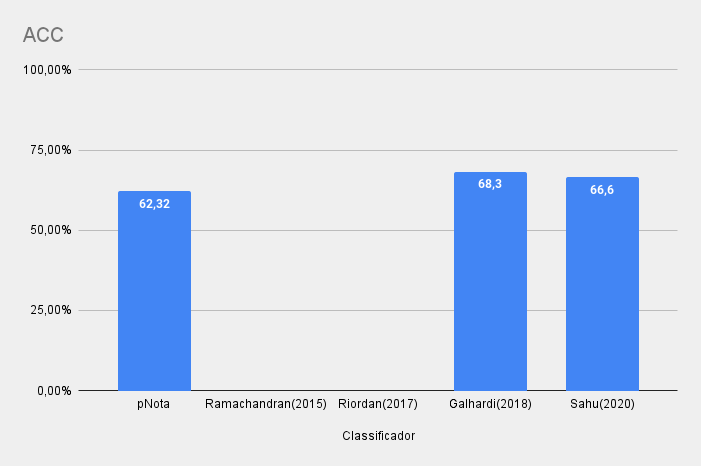
\includegraphics[width=.6\textwidth]{figuras/beetle/res-beetle-acc.png}
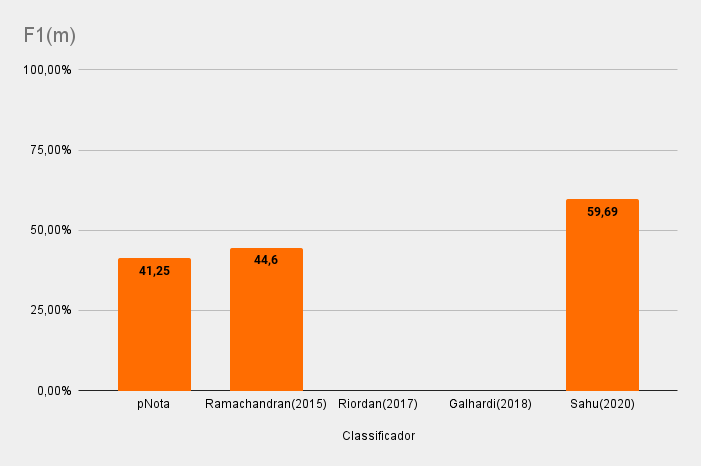
\includegraphics[width=.6\textwidth]{figuras/beetle/res-beetle-mfs.png}
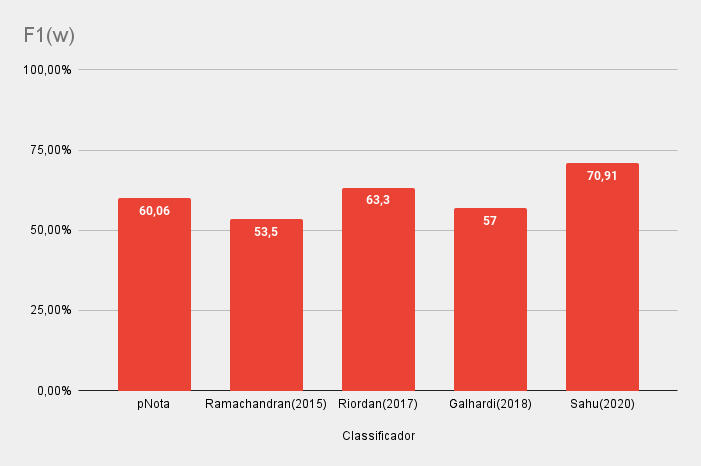
\includegraphics[width=.6\textwidth]{figuras/beetle/res-beetle-wfs.png}
\caption{Resultados obtidos no \textit{dataset} \textit{Beetle}.}
\label{fig-semeval-beetle}
\end{figure}


Na Figura \ref{fig-semeval-beetle}, mostramos o desempenho do \textit{p}Nota e dos trabalhos da literatura em ACC, F1-macro e F1-ponderado. O melhor resultado é apresentado por \cite{sahu2020}, com uma estratégia que realiza a combinação de vários níveis da estrutura textual, atingindo ACC de 66,6\% e F1-ponderado de 70,91\%. Neste, os autores incluem \textit{features} de similaridade semântica, de sobreposição léxica, de recuperação da informação, de similaridade de tópicos, similaridade entre \textit{feedbacks} e de alinhamento textual. Portanto, temos uma ampla aquisição de informação, combinando os métodos tradicionais \textit{Latent Semantic Analysis} (LSA), \textit{word embeddings}, \textit{Recall Oriented Understudy for Gisting Evaluation} (ROUGE), \textit{TF-IDF}, \textit{LDA}, dentre outros. A avaliação é dada posterioremente com ensembles usando \textit{Random-Forest}.

No estudo realizado por \cite{galhardi2018c} encontramos também uma combinação de \textit{features} que incluem estatísticas textuais, como o cálculo de erros, tamanhos de resposta e contagem de palavras por sentença. Essas estruturas eram comuns nos primeiros trabalhos da área, hoje avançando com análise da linguagem \cite{burrows2015}. Usando \textit{Random Forests} e \textit{Extreme Gradient Boosting} os autores alcançaram ACC de 68,3\% e F1-ponderado de 57\%. Um terceiro destaque vale para o trabalho de \cite{riordan2017}, com F1-ponderado de 63,3\%. Nesse caso, os autores não divulgaram as demais métricas. O resultado foi alcançado combinando \textit{word-embeddings}, \textit{Convolutional Neural Networks} (CNN) e \textit{Long Short-Term Memory} (LSTM). As notas são dadas no \textit{layer} de agregação por um modelo linear. Outra técnica aplicada é a sumarização, avaliando as respostas ao mensurar a similaridade dos grafos textuais \cite{ramachandran2015a, ramachandran2015b}. Essa estratégia ainda depende de combinar vários trechos da atividade, desde o enunciado até o quadro de \textit{rubrics}. De forma geral, os resultados obtidos no \textit{Beetle} são bem próximos entre eles. O desempenho intermediário indica o desafio de compreender as 5 categorias do \textit{dataset}. Outra perspectiva é dada nos resultados do \textit{SciEntsBank}, apresentados na Figura \ref{fig-semeval-seb}.

\begin{figure}[!h]
\centering
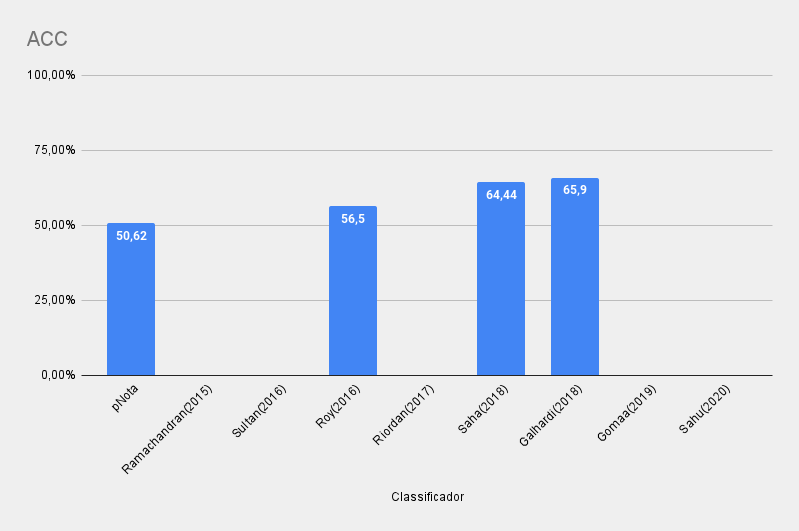
\includegraphics[width=.6\textwidth]{figuras/seb/res-seb-acc.png}
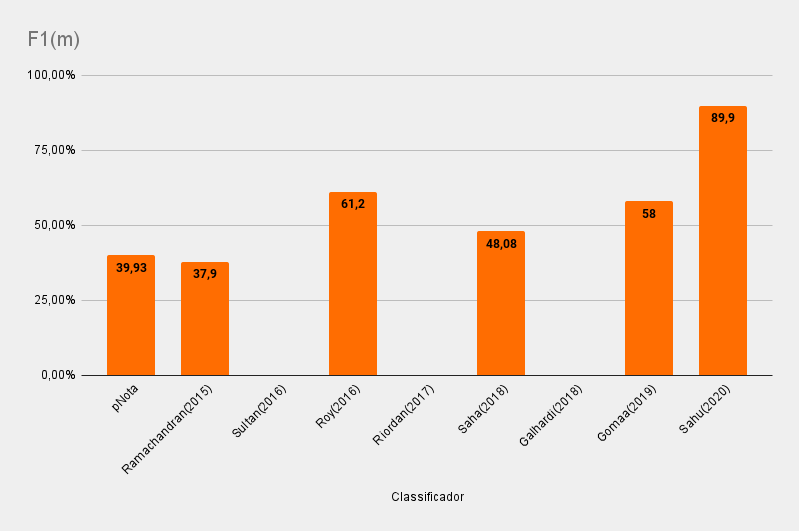
\includegraphics[width=.6\textwidth]{figuras/seb/res-seb-mfs.png}
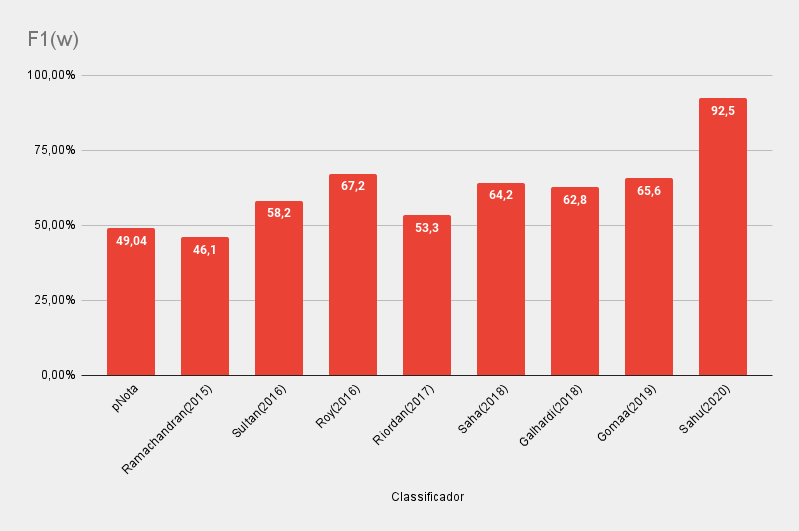
\includegraphics[width=.6\textwidth]{figuras/seb/res-seb-wfs.png}
\caption{Resultados obtidos no \textit{dataset} \textit{SciEntsBank}.}
\label{fig-semeval-seb}
\end{figure}


Na Figura \ref{fig-semeval-seb} vemos que, apesar da aplicação no mesmo desafio, temos vários trabalhos que foram aplicados apenas nesse segundo. O melhor resultado é apresentado por \cite{sahu2020}, com F1-ponderado de 92,5\%. Porém, esse desempenho muito superior é incomum, pois não apresenta o mesmo resultado no \textit{Beetle}. Os autores relatam como maior ganho de desempenho as técnicas de similaridade semântica e sobreposição textual. Portanto, as atividades têm potencial de ter alto desempenho com técnicas de construção de regras e expressões regulares.

O estudo realizado por \cite{roy2016} apresentou ACC de 56,5\% e F1-ponderado de 67,2\%. Tal como mencionado, os autores estudaram técnicas para aquisição de padrões sequenciais, comparando com as respostas candidatas. O método em uma forma geral foi feito no nível de \textit{tokens}, identificando sobreposição entre as respostas. A técnica tem desempenho muito superior em algumas classes, dado o alto F1-ponderado mas acompanhado de um ACC menor que outros trabalhos da literatura. Técnicas mais recentes foram propostas por \cite{galhardi2018c} e \cite{saha2018}. O primeiro alcançou resultados ACC média de 65,9\% e F1-ponderado de 62,8\% usando \textit{Random Forests} e \textit{Extreme Gradient Boosting}. Enquanto o segundo aplicou 6 níveis de análise dos termos, apostando no \textit{Histogram of Partial Similarity}. Este aplica um score de similaridade entre a resposta candidata e cada uma das respostas. As palavras são comparadas pela similaridade de cosseno dos pares em \textit{word embeddings}. 

A aplicação feita com LSTMs realizada por \cite{riordan2017} alcançou F1-ponderado de 53,3\%. Uma proposta parecida foi realizada por \cite{gomaa2019}. Os autores realizam uma composição com vetores semânticos via \textit{skip-thought}, comparando os vetores resiltantes. Os vetores são dados através de pares, pelo produto e pela diferença entre uma resposta e a resposta candidata. O resultado alcançado é de F1-ponderado de 65,6\% em média. 

Pela baixa quantidade de amostras, no \textit{SciEntsBank} os sistemas têm maior dificuldade de adquirir conhecimento por categoria de nota. Por isso, os sistemas que apresentaram melhores resultados foram os que utilizaram a sobreposição dos termos com resposta candidata. No entanto, isto indica que tais estratégias seguem um único viés de resposta, tornando-se menos efetivas ao lidar com variações linguísticas \cite{filighera2020}.

A hipótese que levantamos é que a adição de informação foi um diferencial, dado o pequeno número de amostras por classe. Ao todo, o \textit{SciEntsBank} contém em média apenas 37 respostas por questão, enquanto o \textit{Beetle} apresenta 84 respostas. Dentre as 4380 respostas do \textit{Beetle}, 1841 foram anotadas como \textit{correct}, 1160 como \textit{contradictory} e 1031 como \textit{partially-correct-incomplete}. Por outro lado, apenas 218 foram avaliadas como \textit{non-domain} e 130 como \textit{irrelevant}. Considerando ainda a distribuição de classes, a situação é agravada em relação ao \textit{SciEntsBank}. Dentre as 5509 respostas, 2241 foram dadas como \textit{correct}, 1437 como \textit{partially-correct-incomplete}, 1248 como \textit{irrelevant} e 557 como \textit{contradictory}. Só constam neste \textit{dataset} 26 respostas anotadas como \textit{non-domain} dentre as 143 questões. Notoriamente, são poucas amostras para algumas categorias que se destacam quando vemos que, em média, o primeiro \textit{dataset} apresenta 93 respostas por questão enquanto o segundo apresenta apenas 38 respostas. Portando, apesar da complexidade de avaliar tal questão, os resultados são positivos, aprimorando resultados esperados conforme a distribuição de \textit{clusters}.

Na sequência temos os resultados obtidos com o \textit{dataset} \textit{Open University}. Neste conjunto de dados a avaliação designada foi binária, com notas 0 ou 1. Assim, a avaliação foi dada apenas como corretas ou incorretas. Bem distinta dos \textit{datasets Beetle} e \textit{SciEntsBank}, este conjunto contém mais de 23 mil respostas e, em média, 1190 respostas para cada questão. Isso impacta diretamente na construção de modelos de resposta, com uma variedade de padrões para uma mesma classe, sendo possível a identificação de núcleos de resposta bem consistentes segundo a simetria da classe. Os resultados apresentados na Tabela \ref{tab-OU} refletem justamente este aspecto.

\begin{table}
\centering
\caption{Resultados de classificação para o \textit{dataset OpenUniversity}.}
\label{tab-OU}
\begin{tabular}{l r r r r r}
    \hline
    \multicolumn{4}{l}{\textbf{Open University}} &  \multicolumn{2}{r}{(2 Categorias)} \\ \hline
     & \multicolumn{5}{c}{M{\'e}tricas} \\ \cline{2-6}

     & ACC & PRE & REC & F1(m) & F1(w) \\ \cline{2-6}
    DTR & 96,44\% & 93,66\% & \textbf{93,26\%} & 93,21\% & 96,46\% \\
    GBC & \textbf{96,80\%} & \textbf{96,39\%} & 92,80\% & \textbf{93,64\%} & \textbf{96,60\%} \\
    KNN & 84,62\% & 82,09\% & 78,12\% & 77,50\% & 83,80\% \\
    RDF & 93,62\% & 93,58\% & 88,75\% & 89,79\% & 93,37\% \\
    SVM & 91,45\% & 91,04\% & 85,21\% & 85,41\% & 90,16\% \\
    WSD & 90,44\% & 90,47\% & 84,89\% & 84,78\% & 89,56\% \\

    \hline
    \hline
\end{tabular}
\end{table}

É evidente, através dos resultados obtidos e apresentados na Tabela \ref{tab-OU75}, que a grande quantidade de amostras melhorou consideravelmente o desempenho do sistema. Sendo assim, o \textit{p}Nota atingiu média de 96,8\% de ACC e 96,6\% de F1-ponderado. A simplificação dos padrões de nota para um esquema de avaliação binário é um fator que torna mais simples diferencias o que contribui positivamente e negativamente com cada classe. A Figura \ref{fig-OU} apresenta um comparativo do desempenho do \textit{p}Nota em relação a publicação dos autores.

\begin{figure}[!h]
\centering
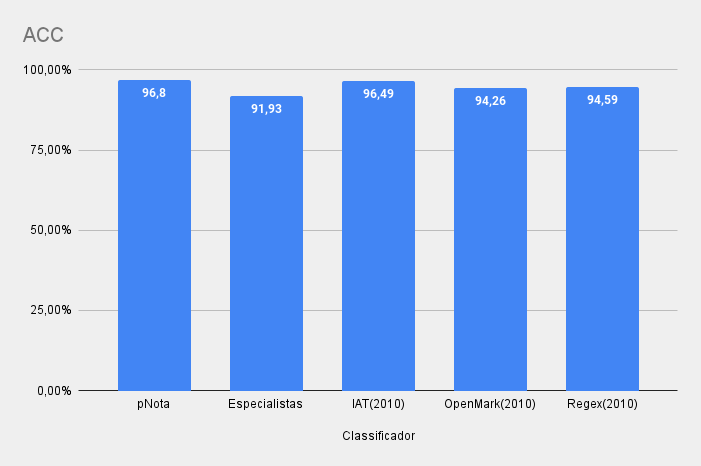
\includegraphics[width=.6\textwidth]{figuras/OU/res-ou-acc.png}
\caption{Resultados obtidos no \textit{dataset} da \textit{Open University}.}
\label{fig-OU}
\end{figure}

A Figura \ref{fig-OU} demonstra a alta qualidade da classificação automática em relação ao que foi reportado entre especialistas. Os especialistas atingiram entre eles ACC média de 91,33\%. Os autores \cite{butcher2010} reportaram ACC de 96,49\%. Porém, os três sistemas aplicados utilizam regras e expressões regulares, o que demanda de maior esforço para inicio das correções. Assim, o sistema deve aguardar enquanto o professor elabora as regras de correção. Como o estudo destaca, o IAT usa o conhecimento sobre o conteúdo e as regras de associação de respostas para criação de \textit{feedbacks} direcionados ao tema.

Outro \textit{dataset} similar é o \textit{Powergrading}. Este \textit{dataset} também conta com muitas amostras e classificação binária. Foi criado por \cite{basu2013} para estudos que aplicam técnicas de clusterização na atribuição de notas. Portanto, uma hipótese é que neste caso há maior separabilidade entre as classes e baixa taxa de sobreposição, algo incomum para respostas discursivas. Os resultados obtidos pelo \textit{p}Nota são apresentados na Tabela \ref{tab-PG}.

\begin{table}
\centering
\caption{Resultados de classificação para o \textit{dataset Powergrading}.}
\label{tab-PG}
\begin{tabular}{l r r r r r}
    \hline
    \multicolumn{4}{l}{\textbf{Powergrading}} & \multicolumn{2}{r}{(2 Categorias)} \\ \hline
     & \multicolumn{5}{c}{M{\'e}tricas} \\ \cline{2-6}

     & ACC & PRE & REC & F1(m) & F1(w) \\ \cline{2-6}
    DTR & 99,79\% & 97,96\% & \textbf{98,68\%} & 98,28\% & 99,80\% \\
    GBC & 99,71\% & 97,46\% & 98,64\% & 97,93\% & 99,74\% \\
    KNN & 99,79\% & 97,96\% & \textbf{98,68\%} & 98,28\% & 99,80\% \\
    RDF & 99,79\% & 97,96\% & \textbf{98,68\%} & 98,28\% & 99,80\% \\
    SVM & \textbf{99,86\%} & \textbf{99,93\%} & 97,50\% & \textbf{98,30\%} & \textbf{99,83\%} \\
    WSD & 99,79\% & 97,96\% & \textbf{98,68\%} & 98,28\% & 99,80\% \\

    \hline
    \hline
\end{tabular}
\end{table}

Como a Tabela \ref{tab-PG75} aponta, alcançamos um bom desempenho com o \textit{p}Nota. Neste, todos os 6 classificadores apresentam apenas erros pontuais, atingindo ACC de 99,86\% e F1-ponderado de 99,83\%. Neste caso, o alto desempenho do SVM reforça a hipótese de baixa sobreposição de \textit{features} entre as classes. Os resultados em relação aos demais trabalhos da literatura são apresentados na Figura \ref{fig-PG}.

\begin{figure}[!h]
\centering
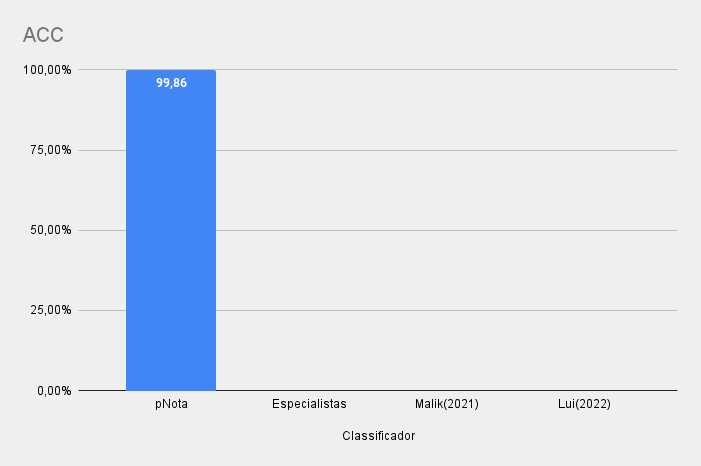
\includegraphics[width=.6\textwidth]{figuras/Powergrading/res-pg-acc.png}
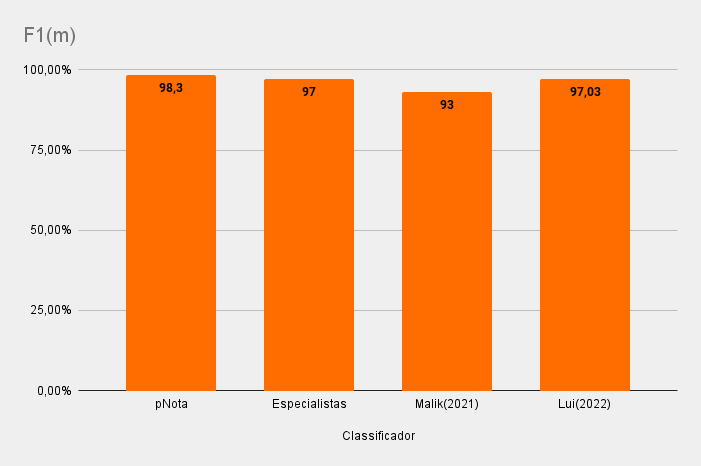
\includegraphics[width=.6\textwidth]{figuras/Powergrading/res-pg-mfs.png}
\caption{Resultados dos classificadores com dados do \textit{dataset} \textit{Powergrading}.}
\label{fig-PG}
\end{figure}

Na Figura \ref{fig-PG} temos um alta qualidade de avaliação entre humanos, mas replicada pelos sistemas. Entre especialistas o F1-macro observado foi de 97\%. O estudo realizado por \cite{malik2021}, com foco na formação de \textit{feedbacks} explicativos. Os autores utilizaram \textit{Deep Learning} para elaborar a \textit{Neural Approximate Parsing with Generative Grading} (GG-NAP), Essa técnica visa decompor as respostas para identificar os trechos que compõe uma resposta correta. Entretanto, o método não foi feito apenas para respostas discursivas, mas também para atividades com linguagens de programação e programação em blocos. O desempenho como avaliador alcançado é de 93\% de F1-macro. 

Outra proposta foi apontada por \cite{lui2022}, usando clusterização e análise de divergências entre as amostras, atingindo F1-macro médio de 97,03\%. O método de clusterização aplicado é um \textit{multi-objective evolutionary clustering}, trabalhando os agrupamentos como uma população, buscando o refinamento para aproximar de uma resposta otimizada por \textit{cluster}. A ideia é aumentar a qualidade dos \textit{clusters} segundo suas menções, elegendo sua representação. Portanto, este conjunto de dados reflete como a etapa de clusterização é efetiva para coleta de informações, recuperando a resposta ideal. Entretanto, por mais que ocorram as subpartições entre \textit{clusters} em ambas as propostas, há preocupação com as características que não encontramos no \textit{dataset} \textit{Powergrading}, como altos índices de \textit{outliers} e a \textit{subjetividade} na avaliação.

Seguindo a mesma plataforma avaliativa, o \textit{PTASAG} foi descrito no trabalho de \cite{galhardi2020}. Neste, os autores investigam o impacto das \textit{features} na formação de um bom avaliador. Os níveis estudados foram representação em \textit{n-grams}, representação em \textit{word embeddings}, similaridade léxica, similaridade em \textit{word embeddings}, similaridade em \textit{WordNet} e estatísticas textuais, apresentando nessa ordem maior qualidade. Nessa linha, foram estudadas técnicas primárias (como o tamanho das respostas) até as técnicas consolidadas de \textit{word embeddings} (Word2Vec, GloVe e FastText). Portanto, o estudo sugere que o maior ganho na avaliação deste \textit{dataset} foi a análise das sequências textuais. O desempenho apresentado pelo \textit{p}Nota é mostrado na Tabela \ref{tab-PTASAG}.

\begin{table}[!h]
\centering
\caption{Resultados de classificação para o \textit{PTASAG}.}
\label{tab-PTASAG}
\begin{tabular}{l r r r r r}
    \hline
    \multicolumn{4}{l}{\textbf{PTASAG}} & \multicolumn{2}{r}{(4 Categorias)} \\ \hline
     & \multicolumn{5}{c}{M{\'e}tricas} \\ \cline{2-6}

     & ACC & PRE & REC & F1(m) & F1(w) \\ \cline{2-6}
    DTR & 88,10\% & 61,39\% & 60,98\% & 60,25\% & 88,01\% \\
    GBC & 90,29\% & 66,14\% & 66,27\% & 64,55\% & 91,07\% \\
    KNN & 87,78\% & 65,77\% & 67,36\% & 64,44\% & 88,46\% \\
    RDF & \textbf{94,49\%} & \textbf{69,04\%} & \textbf{67,98\%} & \textbf{67,32\%} & \textbf{94,05\%} \\
    SVM & 79,13\% & 61,22\% & 61,91\% & 56,55\% & 78,61\% \\
    WSD & 86,33\% & 61,83\% & 62,71\% & 60,48\% & 87,60\% \\

    \hline
    \hline
\end{tabular}
\end{table}

A Tabela \ref{tab-PTASAG} mostra o desempenho da nossa proposta de SAG. Os resultados obtidos mostram alto desempenho com RDF. Nossa técnica atingiu ACC e F1-ponderado de 94,49\% e 94,05\% respectivamente. Comparando com os níveis de F1-macro, podemos considerar que existe um grande desbalanceamento entre os quatro níveis de nota. Assim, o maior desafio encontrado neste \textit{dataset} é aprender a avaliar as categorias com amostragem desbalanceada. Os resultados em relação a outros trabalhos da literatura são apresetados na Figura \ref{fig-PTASAG}.

\begin{figure}[!h]
\centering
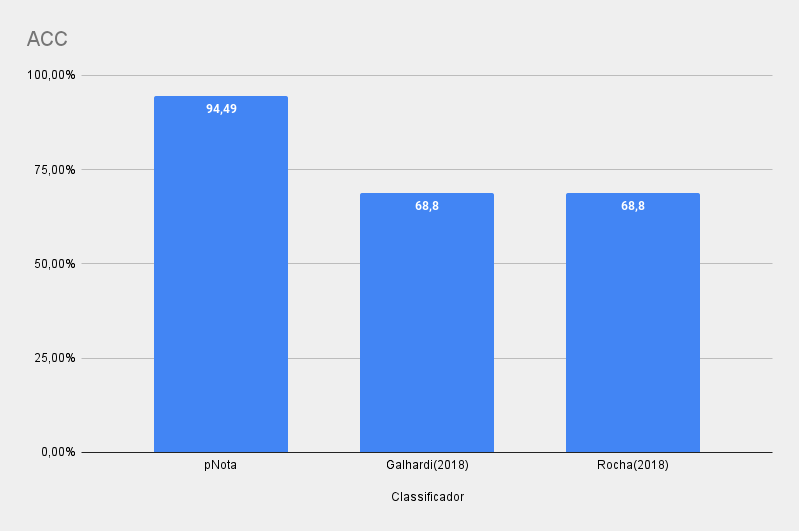
\includegraphics[width=.6\textwidth]{figuras/PTASAG/res-ptasag-acc.png}
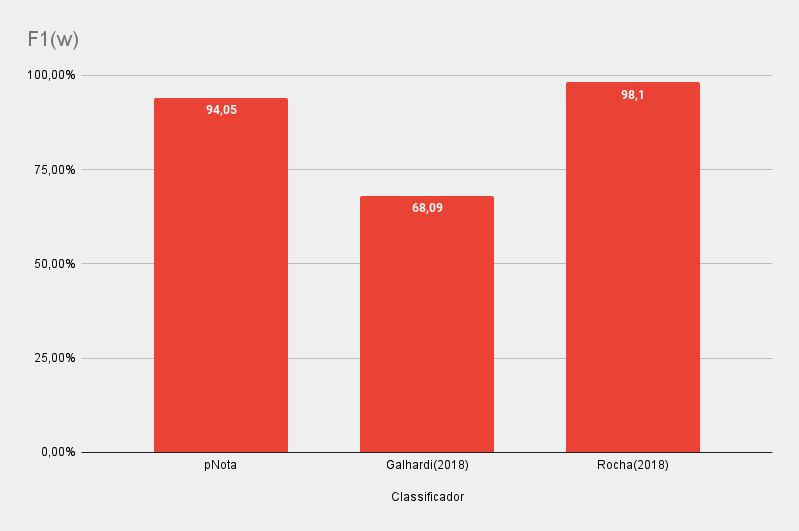
\includegraphics[width=.6\textwidth]{figuras/PTASAG/res-ptasag-wfs.png}
\caption{Resultados dos classificadores com dados do \textit{dataset} \textit{PTASAG}.}
\label{fig-PTASAG}
\end{figure}

Ainda com poucos trabalhos na literatura, a Figura \ref{fig-PTASAG} mostra o desempenho dos estudos realizados no \textit{dataset} \textit{PTASAG}. Nesse estudo, os autores reportaram ACC média de 68,8\% e F1-ponderado de 68,09\% com a tecnica aqui mencionada \cite{galhardi2018b}. Porém, o ganho obtido com as técnicas de \textit{word-embeddings} não foram reportados nas métricas acima, mesmo apresentando um ganho menor do que a análise de \textit{n-grams} \cite{galhardi2020}. Isso acontece pois o coeficiente \textit{kappa} é recomendado para mensurar a equivalência entre pares de avaliadores. Entretanto não permite uma comparação justa com diferentes grupos de amostra.

Em um trabalho mais recente, \cite{gomes-rocha2021} estudou a calibração de oito classificadores para este \textit{dataset}. Dentre os testes estão os classificadores \textit{Logistic Regression}, \textit{K-Nearest Neighbors}, \textit{Support Vector Machines}, \textit{Bernoulli Naive Bayes}, \textit{Extra Trees}, \textit{Random Forest}, \textit{AdaBoost} e \textit{Multi-layer Perceptron}. \textit{Random Forest} apresentou os melhores resultados com ACC de 68,8\%, mas com ganho marginal em relação a outros classificadores. Os autores também apresentam a F1 e PRE acima de 90\%, mas os resultados aparentam incompatibilidade com a ACC descrita.


Este processo de avaliação também ocorre com um dos principais \textit{datasets} da literatura. Com origem em uma competição, o \textit{ASAP-SAS} foi criado com partições fixas de treino e teste, com a proporta de avaliação pelo coeficiente \textit{kappa} quadrático. Os resultados da classificação obtidos pelo \textit{p}Nota são apresentados na Tabela \ref{tab-ASAP-SAS}.


\begin{table}[!h]
\centering
\caption{Resultados de classificação para o \textit{ASAP-SAS}.}
\label{tab-ASAP-SAS}
\begin{tabular}{l r r r r r}
    \hline
    \multicolumn{4}{l}{\textbf{ASAP-SAS}} & \multicolumn{2}{r}{(4 Categorias)} \\ \hline
     & \multicolumn{5}{c}{M{\'e}tricas} \\ \cline{2-6}

    & ACC & PRE & REC & F1(m) &  F1(w) \\ \cline{2-6}
    DTR & 61,03\% & 46,54\% & 47,01\% & 46,39\% & 61,02\% \\
    GBC & \textbf{69,11\%} & \textbf{56,16\%} & \textbf{50,54\%} & \textbf{50,92\%} & \textbf{67,14\%} \\
    KNN & 51,79\% & 38,06\% & 40,36\% & 36,11\% & 52,17\% \\
    RDF & 63,71\% & 51,27\% & 42,19\% & 39,20\% & 57,85\% \\
    SVM & 62,01\% & 44,69\% & 40,29\% & 35,44\% & 54,09\% \\
    WSD & 52,72\% & 44,65\% & 37,39\% & 30,56\% & 48,23\% \\

    \hline
    \hline
\end{tabular}
\end{table}

A Tabela \ref{tab-ASAP-SAS} mostra o desempenho de cada um dos classificadores com o \textit{p}Nota. Um destaque é a grande diferença entre as técnicas, caracterizando a formação de sub-espaços complexos para cada nota. Por conta disso, encontramos uma diferença de 17,32\% entre GBC e KNN, sendo o primeiro o melhor desempenho com ACC de 69,11\% e F1-ponderado de 67,14\%. Entretando, para comparar com a literatura selecionamos os trabalhos que apresentam além do coeficiente \textit{kappa} o nível de erro encontrado na avaliação, com MAE, MSE e RMSE, mesmo sendo um \textit{dataset} com notas discretas. Assim, o nível de erro apresentado na literatura são descritos na Figura \ref{fig-ASAP-SAS}.

\begin{figure}[!h]
\centering
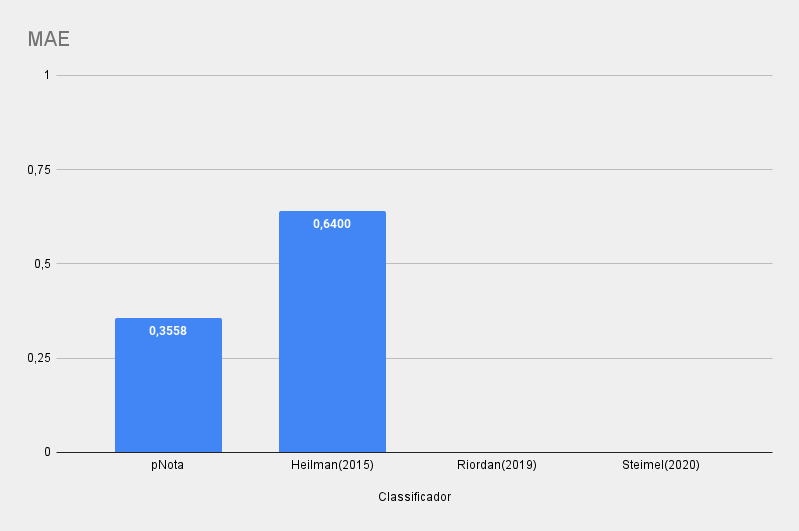
\includegraphics[width=.6\textwidth]{figuras/ASAP/res-asap-mae.png}
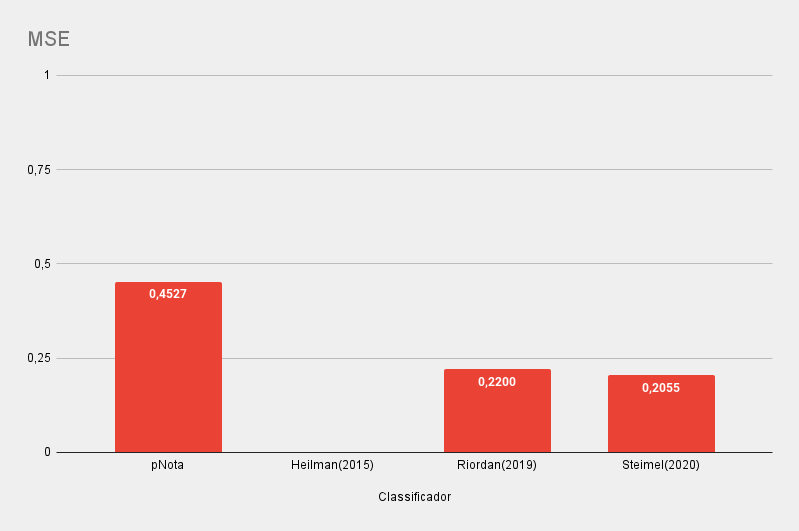
\includegraphics[width=.6\textwidth]{figuras/ASAP/res-asap-mse.png}
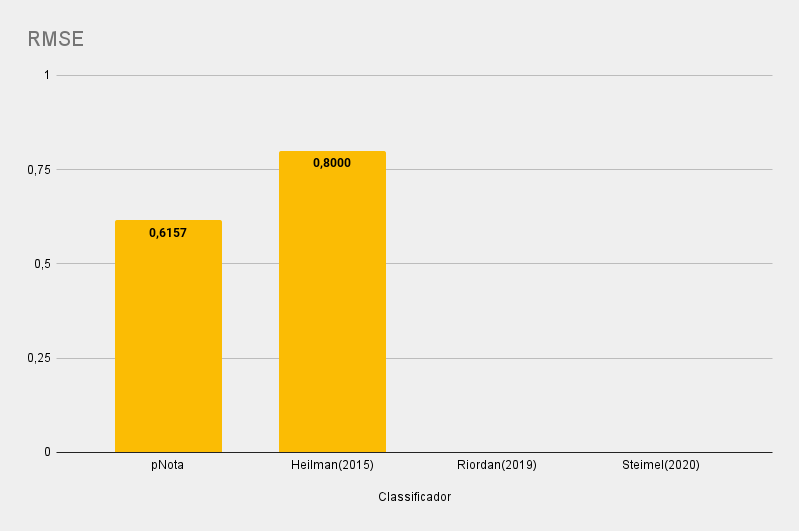
\includegraphics[width=.6\textwidth]{figuras/ASAP/res-asap-rmse.png}
\caption{Resultados dos classificadores com dados do \textit{dataset} \textit{ASAP-SAS}.}
\label{fig-ASAP-SAS}
\end{figure}

Como a Figura \ref{fig-ASAP-SAS} destaca, o nível de erro apresentado pelo \textit{p}Nota é de 0,3558 pontos de MAE e 0,4527 pontos de MSE. As notas deste \textit{dataset} vão de 0 até 3 pontos. Portanto, o erro resultante leva em conta que não existe gradação entre as 4 classes de nota. O melhor resultado é apresentado por \cite{steimel2020}, com MSE de 0,2055 pontos. Os autores aplicaram \textit{Deep Learning}, utilizando \textit{BERT}, uma \textit{bidirectional transformer} com 12 \textit{layers}. A principal mudança aplicada foi o teste de \textit{mean} e \textit{max-pooling} no lugar do padrão aplicado pela rede. Esse trabalho apresenta um ganho interessante em relação ao trabalho anterior dos autores \cite{riordan2019}. Neste primeiro, foi utilizada uma \textit{bidirectional Gated Recurrent Unit}, pré-treinada em uma \textit{word-embeddings}. O principal diferencial deste estudo é a combinação de representações dos documentos (palavras e caracteres) em \textit{Multilayer Perceptron Attention}.

Outro trabalho realizado foi apresentado por \cite{heilman2015}. Neste estudo foi aplicado \textit{Support Vector Regression}, combinando estruturas sintáticas e semânticas. Para entender a influência de algumas respostas no treinamento, foram replicadas as amostras como forma de reforço. No entanto, os resultados obtidos indicam MAE de 0,64 pontos e um RMSE de 0,80 pontos.

Na mesma linha das avaliações contínuas também temos o \textit{dataset} da \textit{University of North Texas}. Esse \textit{dataset} é bem diferente, com apenas 30 respostas por questão. Cada questão foi avaliada por dois avaliadores, \textit{Avaliador1} e \textit{Avaliador2}, em notas de 0 a 5 discretas. Porém, o objetivo é minimizar o erro para a \textit{Média} extraída entre eles. A Tabela \ref{tab-UNT} detalha os resultados obtidos via técnicas de regressão para cada uma das 3 avaliações.


\begin{table}[!h]
\centering
\caption{Índices de erro obtidos em cada um dos cenários de avaliação do \textit{dataset} da \textit{University of North Texas}.}
\label{tab-UNT}
\begin{tabular}{p{5cm} r r r }
    \hline
    \multicolumn{3}{l}{\textbf{University of North Texas}} & (Notas 0 - 5) \\ \hline
     & \multicolumn{3}{c}{M{\'e}tricas} \\

    & \multicolumn{3}{l}{Avaliador1} \\ \cline{2-4}
     & MAE & MSE & RMSE \\
    LINR & 1,0066 & \textbf{2,5069} & \textbf{1,1955} \\
    LSSR & 1,3273 & 3,1713 & 1,4712 \\
    KNRG & 0,9366 & 2,9032 & 1,2557 \\
    DTRG & \textbf{0,9233} & 3,7338 & 1,4482 \\
    WSRG & 1,2832 & 3,0113 & 1,4240 \\
    \\
    & \multicolumn{3}{l}{Avaliador2} \\ \cline{2-4}
     & MAE & MSE & RMSE \\
    LINR & \textbf{0,4752} & \textbf{0,6099} & \textbf{0,6119} \\
    LSSR & 0,6502 & 0,8605 & 0,7640 \\
    KNRG & 0,4917 & 0,7550 & 0,6658 \\
    DTRG & 0,5121 & 1,2002 & 0,7856 \\
    WSRG & 0,6523 & 0,8839 & 0,7680 \\
    \\
    & \multicolumn{3}{l}{Média} \\ \cline{2-4}
     & MAE & MSE & RMSE \\
    LINR & \textbf{0,5058} & \textbf{0,5476} & \textbf{0,6199} \\
    LSSR & 0,7299 & 0,8464 & 0,8170 \\
    KNRG & 0,5055 & 0,6804 & 0,6765 \\
    DTRG & 0,5811 & 1,1244 & 0,8372 \\
    WSRG & 0,7024 & 0,8088 & 0,7920 \\

    \hline
    \hline
\end{tabular}
\end{table}

A Tabela \ref{tab-UNT} mostra o nível de erro para cada avaliação, com destaque para a \textit{Média}. O \textit{p}Nota apresenta MAE de 0,5058, MSE de 0,5476 e RMSE de 0,6199 pontos. Por conta dessa baixa quantidade de amostras, temos um problema na comparação com os demais estudos da literatura. Alguns métodos utilizam até 12-\textit{Fold} durante a avaliação \cite{kumar2017, saha2018}. No caso do \textit{p}Nota, com treino fixado pelo método de clusterização, aplicamos aqui 75\% das amostras para treinamento tal qual encontramos em outros \textit{datasets} da literatura.

\begin{figure}[!h]
\centering
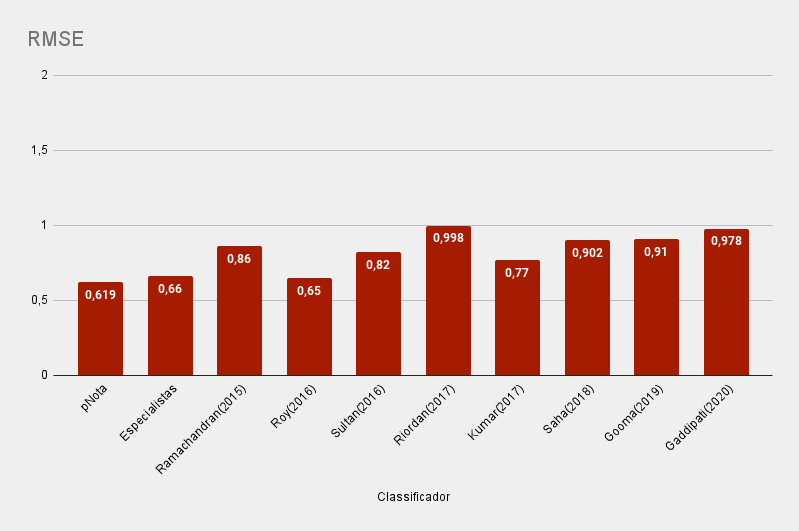
\includegraphics[width=.6\textwidth]{figuras/UNT/res-unt-rmse.png}
\caption{Resultados dos avaliadores com dados do \textit{dataset} \textit{University of North Texas}.}
\label{fig-UNT}
\end{figure}


Na Figura \ref{fig-UNT} mostra um detalhe interessante na evolução dos sistemas SAG. Os sistemas mais recentes, em ordem da esquerda para direita, aumentaram consideravelmente o erro nesse \textit{dataset}. Nesse cenário, o menor erro encontrado foi obtido pelo \textit{p}Nota, com apenas 0,619 pontos de RMSE para a média dos avaliadores. Isso acontece com os métodos já descritos \cite{riordan2017, saha2018, gomaa2019, ramachandran2015b}. 

A divergência observada entre os especilistas neste \textit{dataset} foi de 0,66 pontos. Apenas o trabalho descrito por \cite{roy2016} chegou nesse nível, com RMSE de 0,65 pontos. Seu diferencial, como comentado anteriormente, foi uma métrica de sobreposição entre respostas, calculando equivalência e divergências entre as respostas. Em um trabalho mais elaborado, \cite{kumar2017} atingiu 0,77 pontos de RMSE com uma técnica específica de \textit{pooling} aplicada em \textit{Siamese LSTMs}. Para reforço do aprendizado com poucas amostras, os autores utilizaram \textit{data aumentation}. Enquanto uma LSTM trabalha no \textit{encodding} da resposta candidata, a segunda realiza o \textit{encodding} das respostas dos alunos. O \textit{layer} que avalia a compatibilidade utiliza a \textit{Earth mover distance pooling}. Esta distância calcula a transferência mínima para aproximar os dois vetores na comparação de sequencias em \textit{word embeddings}.

O trabalho mais recente de \cite{gaddipati2020} mostra uma comparação do desempenho de modelos de \textit{Transfer Learning}. Dentre eles temos o ELMo, GPT, GPT-2 e BERT. Os autores utilizaram 70\% dos dados para treino e 30\% para teste. Os autores compararam os resultados com outros métodos de análise vetorial tradicionais como TF-IDF, \textit{Word2Vec}, \textit{GloVe} e \textit{FastText}. O melhor resultado obtido foi com o ELMO, com 0,978 pontos de RMSE. Ainda neste estudo os autores destacam o problema do desbalanceamento das notas, com média de 4,17 pontos por resposta. Tornando bem complexa a tarefa de aprendizado para níveis menores de nota.

Outros dois \textit{datasets} aplicados foram com dados locais. O \textit{dataset} \textit{VestUFES} foi utilizado durante os anos para o desenvolvimento do \textit{p}Nota \cite{spalenza2017}. Este primeiro é aplicado com dados do vestibular da universidade. Ele contém notas normalizadas para a escala de 0 a 10, mas foi avaliador inicialmente em notas contínuas entre 0 e 2 pontos. Os resultados de avaliação do \textit{p}Nota são apresentados na Tabela \ref{tab-VEST}.

\begin{table}[!h]
\centering
\caption{Índices de erro obtidos em cada um dos cenários de avaliação do \textit{dataset} do \textit{VestUFES}.}
\label{tab-VEST}
\begin{tabular}{p{5cm} r r r }
    \hline
    \multicolumn{3}{l}{\textbf{VestUFES}} & (Notas 0 - 10) \\ \hline
     & \multicolumn{3}{c}{M{\'e}tricas} \\

    & \multicolumn{3}{l}{Avaliador1} \\ \cline{2-4}
     & MAE & MSE & RMSE \\
    LINR & 1,8614 & \textbf{6,0562} & \textbf{2,3261} \\
    LSSR & 2,4570 & 9,5859 & 2,9596 \\
    KNRG & 1,9058 & 6,8529 & 2,5057 \\
    DTRG & \textbf{1,6348} & 7,0130 & 2,5333 \\
    WSRG & 2,4665 & 9,6489 & 2,9515 \\
    \\
    & \multicolumn{3}{l}{Avaliador2} \\ \cline{2-4}
     & MAE & MSE & RMSE \\
    LINR & 1,7943 & \textbf{5,2526} & \textbf{2,1898} \\
    LSSR & 2,4358 & 8,5399 & 2,8264 \\
    KNRG & 1,7290 & 6,3471 & 2,3781 \\
    DTRG & \textbf{1,6783} & 7,7696 & 2,6739 \\
    WSRG & 2,4282 & 8,5112 & 2,8111 \\

    & \multicolumn{3}{l}{Final} \\ \cline{2-4}
     & MAE & MSE & RMSE \\
    LINR & 1,8556 & \textbf{5,4816} & \textbf{2,2326} \\
    LSSR & 2,5365 & 9,5175 & 2,9435 \\
    KNRG & \textbf{1,7667} & 6,7042 & 2,3789 \\
    DTRG & 1,8457 & 8,3614 & 2,6566 \\
    WSRG & 2,5256 & 9,4779 & 2,9198 \\

    \hline
    \hline
\end{tabular}
\end{table}

A Tabela \ref{tab-VEST} mostra resultados distintos entre as notas individuais dos avaliadores e o resultado médio. Tanto para o \textit{Avaliador 1} quanto para o \textit{Avaliador 2}, o menor nível de erro observado em MAE foi dado pelo DTRG. No entanto, para a nota média o KNRG apresentou melhor desempenho com MAE de 1,7667 pontos.

O segundo \textit{dataset} local foi desenvolvido em 2019 para retratar um pouco melhor os resultados em dados nacionais. O \textit{dataset} do \textit{Projeto Feira Literária} foi coletado em conjunto com os autores para descrição da aplicação do \textit{p}Nota e seu uso por professores \cite{nascimento2020}. Este caracteriza-se pela presença de erros de escrita e conteúdos fora de tópico, sendo fatores avaliados negativamente pelo tutor. A Tabela \ref{tab-FINDES} caracteriza o desempenho de cada um dos seis classificadores e seus resultados alcançados na avaliação das questões do projeto.


\begin{table}[!h]
\centering
\caption{Resultados de classificação para o \textit{Projeto Feira Literária}.}
\label{tab-FINDES}
\begin{tabular}{l r r r r r}
    \hline
    \multicolumn{4}{l}{\textbf{Projeto Feira Literária}} & \multicolumn{2}{r}{(4 Categorias)} \\ \hline
     & \multicolumn{5}{c}{M{\'e}tricas} \\ \cline{2-6}

     & ACC & PRE & REC & F1(m) & F1(w) \\ \cline{2-6}
    DTR & 77,86\% & 59,99\% & 59,29\% & 58,42\% & 76,84\% \\
    GBC & \textbf{78,58\%} & 59,58\% & 59,57\% & 57,07\% & \textbf{77,74\%} \\ 
    KNN & 65,00\% & 58,72\% & 58,02\% & 54,75\% & 66,91\% \\
    RDF & 78,57\% & \textbf{61,82\%} & \textbf{64,98\%} & \textbf{61,36\%} & 76,53\% \\
    SVM & 72,86\% & 51,49\% & 57,85\% & 49,34\% & 67,66\% \\
    WSD & 75,71\% & 54,77\% & 61,24\% & 56,14\% & 74,57\% \\

    \hline
    \hline
\end{tabular}
\end{table}

Conforme a Tabela \ref{tab-FINDES}, temos alta qualidade de de três classificadores RDF, DTR e GBC. Esse último, em especial, teve o maior desempenho com 78,58\% de ACC. Com 70 respostas e a pluralidade de estruturas textuais encontradas, destacamos a semelhança deste com o desafio de correção dos datasets \textit{Beetle} e \textit{SciEntsBank} no ensino de ciências.

\section{Discussão de Resultados}
\label{sec-discussao}

Os sistemas SAG apresentam uma diversidade de características, com diferentes estudos e técnicas aplicadas. É uma área que evoluiu muito com o tempo, principalmente com a adoção em massa do EaD. Dos sistemas mais rígidos, que operam com regras e padrões pré-fixados, até hoje com maior profundidade dos modelos com análises de NLP. Isso inclui técnicas de ML e \textit{Deep Learning} aparecendo nos trabalhos mais recentes. Essas características também são um reflexo dos \textit{datasets}, com diferentes formas de escrita e avaluação. Tornando a verificação textual mais complexa e com necessidade de critérios mais robustos de avaliação.

De qualquer forma, pela dinâmica dos trabalhos na área, vemos que é muito complexa a tarefa de se adequar a todos os cenários. Nessa perspectiva, vemos um ótimo desempenho do \textit{p}Nota, sendo equiparável aos resultados da literatura em todos os cenários testados. O vínculo do método avaliativo com as características textuais encontrado no \textit{p}Nota têm maior capacidade de resolver questões do que boa parte dos sistemas da literatura. Isso porquê a proposta aqui descrita busca compreender diferenças encontradas nos dados antes do processo avaliativo. De forma geral, a preocupação com a modelagem do critério avaliativo torna mais efetiva a contextualização sobre o tema. Portanto, um sistema contextualizado tende a aparesentar bom desempenho como avaliador.

Além disso, o sistema precisa de apenas algo entre 6 minutos e 1 hora para processamento em um computador comum. Essa \textit{performance} foi avaliada em um computador XXX. O tempo de execução é definido segundo o número de etapas e o número de características encontradas nas amostras do conjunto de dados. Desconsideramos nesse cálculo o tempo de anotação do professor. Logo, esse tipo de sistema deve atender ao problema e, simultâneamente, ser associado a rotina de avaliação do professor.

Assim, na criação do modelo linguístico, de uma forma geral os sistemas trabalham o alinhamento entre o conjunto de respostas e as respostas candidatas. Entretanto, a proposta apresentada neste trabalho busca iterações com o professor para evolução do modelo criado. Para além da análise textual o sistema prioriza a conexão entre conteúdo e critério avaliativo. Deste modo, as nuances do contexto são interpretadas pelo tutor durante a avaliação, destacada com o critério de atribuição de notas. Superdimensionados para a avaliação de uma determinada disciplina ou tema, os modelos rígidos divergem bastante da aplicação dos sistemas SAG no cotidiano do professor. Assim, o professor espera que o sistema seja capaz de reduzir o esforço de correção, dando suporte ao seu método assim que requisitado. Portanto, independente do cenário ao qual é aplicado, o sistema SAG deve lidar com as respostas como parte do ensino-aprendizagem, buscando minorar a demanda de verificação do conteúdo.

Ainda é importante salientar que, dentre todas as comparações criadas com os \textit{datasets} disponíveis, o modelo proposto neste trabalho foi o mesmo aplicado para todas as questões. Enquanto isso, parte dos trabalhos são rígidos e contextuais, direcionados a domínios específicos ou dependentes de regras. Por conta disso, inclui-se na qualidade dos resultados obtidos a capacidade do próprio sistema na adaptação ao tema e ao modelo de avaliação. Sendo parte das etapas do \textit{p}Nota a calibração dos processos.

Portanto, a escolha dos modelos segundo seu alinhamento com a avaliação humana acrescenta fluidez na correção. Tornamos o \textit{p}Nota flexível para buscar estudar o contexto aplicado a cada questão. A tendência, então, é que os métodos selecionados, sejam de classificação ou de regressão, apresentem o melhor desempenho. Fazendo parte do ciclo avaliativo, o professor continuamente realiza a audição dos resultados e aplicando os ajustes necessários. Conforme os resultados estejam adequados para a disciplina, a ideia é que a ferramenta colabore também em sala de aula, apoiando os resultados com \textit{feedbacks} direcionados.
% ==============================================================================
% TCC - Nome do Aluno
% Capítulo 3 - Considerações Finais
% ==============================================================================
\chapter{Considerações Finais}
\label{cap-conclusao}

O processo de avaliação de questões discursivas compreende um longo ciclo, da formulação das atividades até a análise de desempenho. Por meio das avaliações acontece o redimensionamento das práticas de ensino e aprendizagem. Assim, a dinâmica avaliativa do professor é uma componente que permite a compreensão e identificação dos \textit{gaps} de aprendizagem. A avaliação também indica formas de refinar a disciplina conforme o desempenho de cada estudante e cada turma, então, é fundamental a produção de técnicas que reduzam o esforço do professor para aplicação cotidiana das atividades.

Em especial, a aplicação de atividades que contribuem para melhoria da leitura e da escrita é essencial para todos os níveis de instrução dos estudantes. Assim, essa aplicação contínua tem benefícios para todos os participantes do ciclo avaliativo. Cientes disso, foi apresentado neste trabalho um estudo de aplicação de métodos de \textit{Active Learning} para suporte ao critério avaliativo do professor. Como destaques dos resultados obtidos com este trabalho foram listadas uma série de contribuições que compõem este estudo:

\begin{itemize}
  \item Aplicação de técnicas de \textit{Active Learning} para refinamento dos ciclos avaliativos;
  \item Dinâmica de otimização dos ciclos de clusterização e classificação para análise da distribuição das amostras e de suas componentes;
  \item Proposta de amostragem guiada pela representatividade de cada amostra no \textit{cluster} que esta compõe;
  \item Modelo de linguagem formado por sequências de estruturas textuais para caracterizar padrões de resposta superiores ao nível de \textit{token};
  \item Reconhecimento de padrões que combinam a interação entre estudantes, o professor e o sistema na avaliação, detalhando o critério segundo o alinhamento ao tema;
  \item Criação de formatos próprios para relatórios e \textit{feedbacks} para descrição do vínculo entre termos e notas.
\end{itemize}

\newpage

\section{Conclusões}

O suporte computacional do processo avaliativo compõe importante parte da integração do ensino em meio digital. O meio digital visa tornar prático e rápido o processo de avaliativo, possibilitando sua aplicação em massa. Desse modo, o professor em um mesmo ambiente consegue interagir com todos os seus alunos e acompanhar seu desempenho na disciplina. 

Por meio dessas plataformas de ensino, possibilita-se o emprego de múltiplas técnicas de EDM para análise do conteúdo e, consequentemente, o aumento da capacidade avaliativa. Este trabalho apresenta um estudo profundo do ciclo avaliativo para integração humano-máquina na correção de respostas discursivas via \textit{Active Learning}. Ao longo do trabalho foi descrito o \textit{p}Nota. O \textit{p}Nota é um sistema para construção de modelos avaliativos que interage diretamente com o tutor para compreender seu critério avaliativo sobre um conjunto de resposta. Integram o sistema vários módulos que, em sequência, realizam o reconhecimento de padrões e identificação contextual.

O método elabora uma forma de interagir com o professor para criação de modelos textuais para representar cada nota. O modelo alcançou níveis similares aos observados entre humanos na qualidade de atribuição de notas, com F1-ponderado médio de 78\% e ACC de 79\%. Destaca-se que tais valores refletem que, das 255 atividades de classificação, 137 foram avaliadas com mais de 75\% nessa métrica. O mesmo desempenho também se reflete nas atividades de regressão, com erros menores do que observados entre humanos nos \textit{datasets} do teste. Com esse modelo é possível que o professor atue com o sistema, corrigindo atividades e utilizando os resultados em função do desenvolvimento de seus métodos de ensino. Adicionalmente, com os \textit{feedbacks}, esperamos compor materiais que auxiliem várias etapas do método avaliativo, incluindo a discussão de resultados em sala.

\section{Trabalhos Futuros}

Em uma perspectiva de próximos estudos em torno do modelo proposto, destacam-se alguns trabalhos ainda de refinamento do modelo. O ganho analítico dos modelos de linguagem e domínio, em especial com \textit{word embeddings}, pode proporcionar novas formas de conhecimento. Mesmo atingindo resultados melhores do que os trabalhos da literatura que apresentam tais características, unindo tais modelos pode-se ter um ganho importante com contextualização. Em uma outra vertente, também são válidos os esforços para entender as variações textuais encontradas em novas iterações de aplicação das atividades. Inclusive, são necessários estudos que caracterizem melhor a evolução do aprendizado.

Outra característica importante para evolução do modelo é a integração de critérios mais sofisticados na otimização dos resultados, para clusterização, classificação e regressão. Tais métodos podem ser relevantes para alcançar ainda mais qualidade na atribuição de notas, inclusive compreendendo a formação de cada conjunto de respostas. Nessa mesma linha, são fundamentais o acompanhamento do sistema em características de usabilidade. Portanto, além de conhecer a prática e os ciclos avaliativos também devemos considerar ter mais proximidade nas iterações sob a ótica do professor. Em especial, é necessário contemplar em detalhes o acompanhamento de escolas, turmas ou grupos de alunos sob a concepção das técnicas de ensino-aprendizagem. Nesse aspecto, é desejável a melhoria da contextualização dos documentos, com o detalhamento da produção escrita e dos ciclos de aplicação das atividades.

%%% Páginas finais do documento: bibliografia e anexos. %%%

% Finaliza a parte no bookmark do PDF para que se inicie o bookmark na raiz e adiciona espaço de parte no sumário.
\phantompart

% Marca o início dos elementos pós-textuais.
\postextual

% Referências bibliográficas
\bibliography{bibliografia}


% Apêndices.
\begin{apendicesenv}

% Imprime uma página indicando o início dos apêndices.
\partapendices


%
% Apêndices
%
\chapter{Relatorios \textit{p}Nota}
\label{exemplo-pNota}

O \textit{p}Nota tem uma série de relatórios que são utilizados para demonstrar o \textit{status} da avaliação e capacitar a auditoria do processo. Nesse constam os seguintes itens:

\begin{itemize}
\item Lista de Requisição de Amostras
\item Distribuição de \textit{Clusters} de Documentos
\item Distribuição de Treino
\item Distribuição de Características
\item Frequência dos Termos
\item Rubricas por Nota
\item Resultados de Classificação
\item Gráficos de Desempenho
\item Matriz de Confusão
\item Árvore de Decisão
\end{itemize}

Para ilustrar os resultados obtidos com o \textit{p}Nota vamos utilizar um pequeno exemplo. O exemplo é dado pela \textit{Atividade 08b}, extraído do \textit{dataset} do Projeto Feira Literária das Ciências Exatas. O enunciado da questão é dado a seguir:

\begin{quote}
\interlinepenalty=10000
\textit{Em eventos e festas, é comum as pessoas colocarem sal grosso sobre blocos de gelo para manter a temperatura. Por que essa ação mantém o gelo?.}
\end{quote}

A seguir é apresentado o arquivo completo de relatórios e \textit{feedbacks} gerados durante o processo.

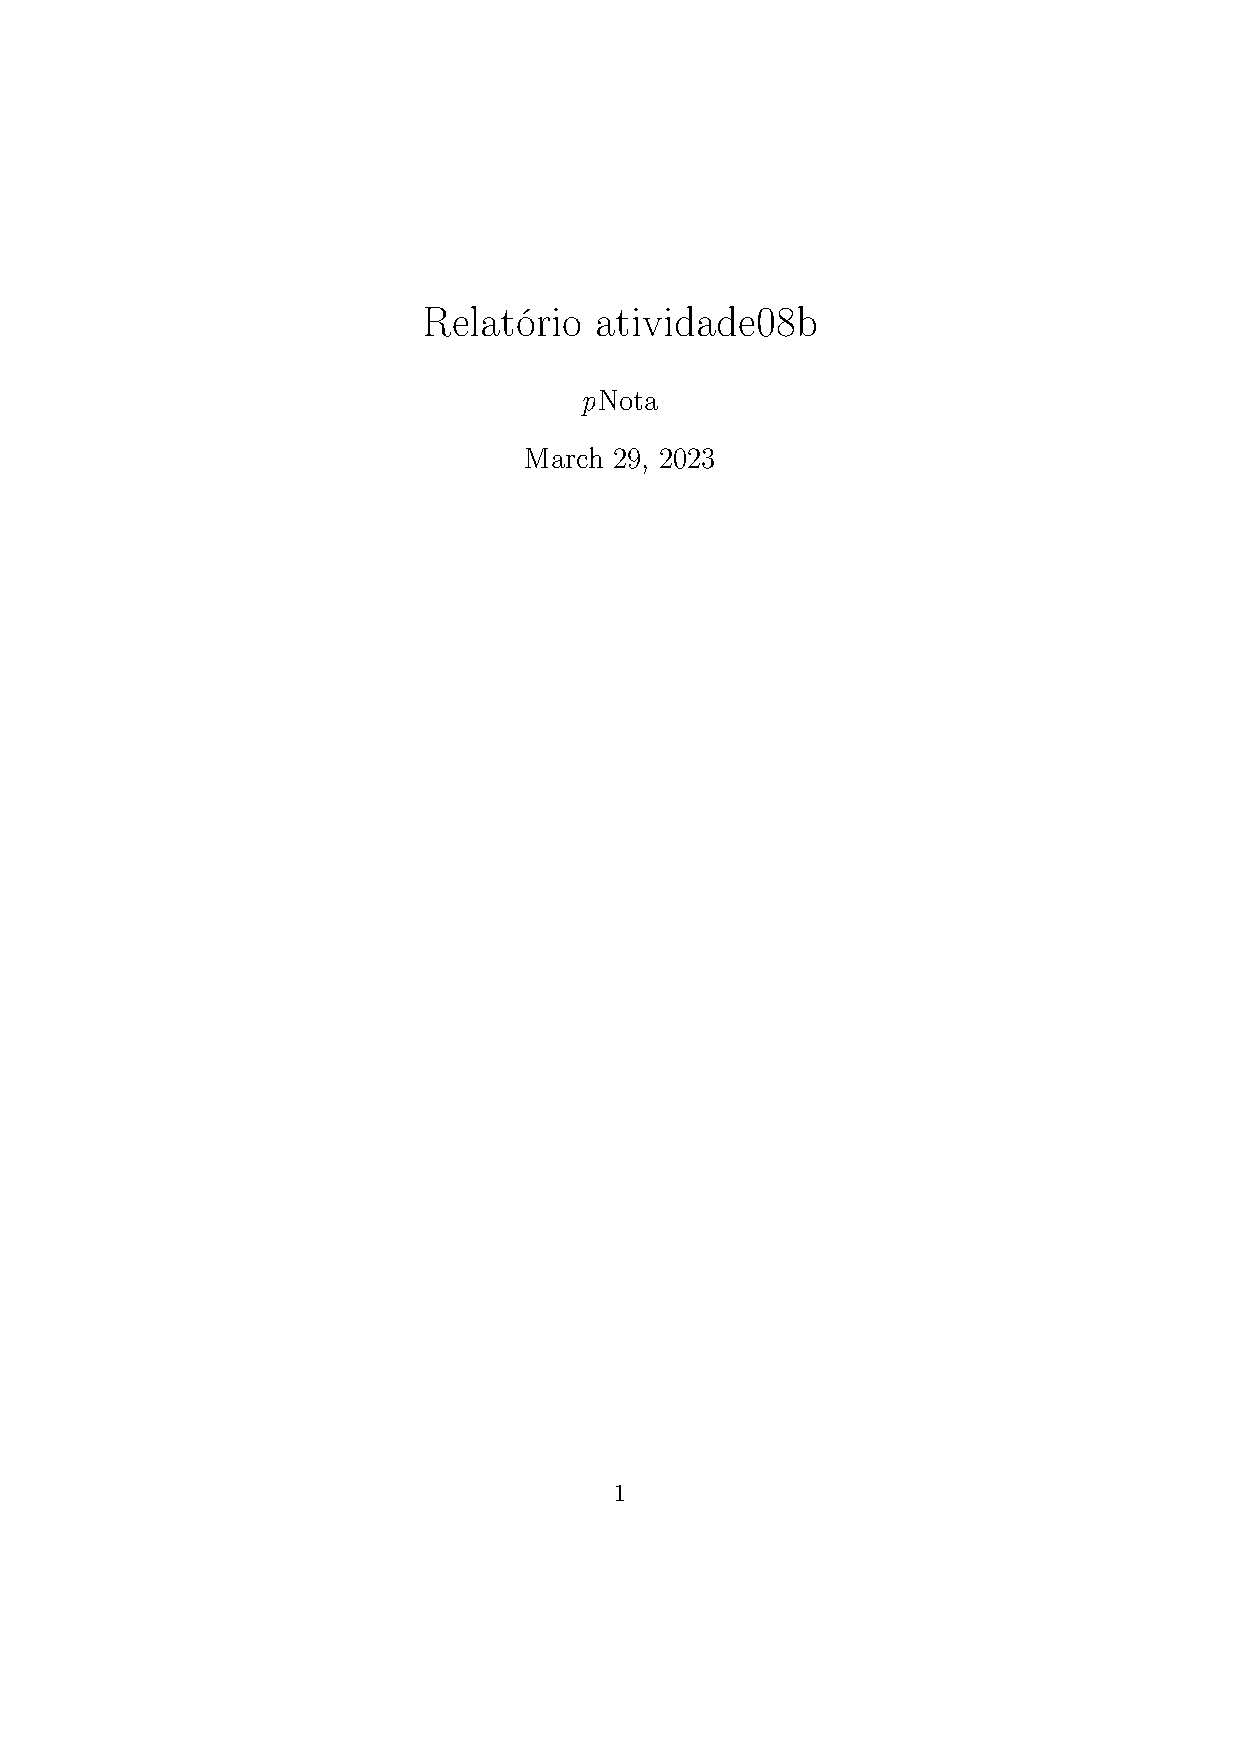
\includepdf[pages={1-}]{relatorio-pNota.pdf}

\end{apendicesenv}


% Índice remissivo.
\phantompart
\printindex

% Fim do documento.
\end{document}